\chapter{CMS Searches for Supersymmetry at $\sqrt{s}=13$ TeV}
\label{chap:susysearches}
One of the findings of Chapter~\ref{chap:run1pmssm}, and seen in Fig.~\ref{fig:Z}, is that searches for SUSY events with purely hadronic final states have a particularly significant impact on our knowledge of the MSSM. Furthermore, it was found that SUSY models characterized by large fiducial cross sections corresponding to low thresholds on the $\met$, $\Ht$, and $\njets$ survived 7 and 8 TeV CMS searches. 

After making these findings, I contributed to CMS hadronic analyses \cite{Khachatryan:2016kdk} and \cite{CMS:2016nhb}, where I developed methods that increase the sensitivity of the searches to SUSY models that predict large numbers of events produced in the low-$\met$ and low-$\Ht$ regions. The primary backgrounds in these regions are multi-jet events arising from QCD interactions, and events arising from the electroweak production of a Z boson that decays into neutrinos, Z$\rightarrow\nu\bar{\nu}$. I developed a data-driven QCD event simulator, based on the rebalance and smear method, that allows the prediction of QCD background counts to be made with uncertainties that are lower than those of alternative methods by up to an order of magnitude. I developed and performed a data-driven $\zinv$ background estimation method that uses events in which a Z boson is produced and decays into two electrons or two muons as a proxy for $\zinv$ background events. I also built upon a technique that maximizes the usefulness of triggers in kinematic regions in which the trigger is not fully turned on. 

The above techniques are discussed generally in the following sections, that is, they are discussed as stand-alone methods, independent of a particular analysis, with only occasional reference made to the analyses in which the methods were applied. The aim of this approach is to accentuate the universality of the techniques. Moreover, special effort was paid to ensure that the methods remain valid in kinematics regions with lower $\met$ and $\Ht$ than the baseline regions of the hadronic analyses, and the methods are used in the next chapter in a new context. Section \ref{sec:2015results} discusses how these methods have been applied specifically in the context of two high-$\met$ hadronic searches: the multi-jet + $\mht$ search \cite{Khachatryan:2016kdk}, and the search for SUSY with top squarks \cite{CMS:2016nhb}. Section \ref{sec:2015results} gives a brief introduction to the analyses \cite{Khachatryan:2016kdk} and \cite{CMS:2016nhb}, a detailing of the baseline selection for each, a discussion of the background estimates and uncertainties obtained using the above methods, and the final results of the searches, namely, limits on sparticle masses set in the context of simplified models.  Then, in the chapter that follows, the use of multivariate techniques in background-dominated kinematic regions like the low-$\met$ region and the low-$\Ht$ region is explored as a way to probe nonexcluded pMSSM points. 


\section{Trigger methods}
\label{sec:anatrig}
\label{sec:hadronictrigger}
Triggers suitable for hadronic SUSY searches at the LHC typically manage to suppress the overwhelming QCD background by requiring events to have a large $\met$ as a criterion for firing the trigger. Additionally, a minimum amount of $\Ht$ can also be required, or, for that matter, some combination of $\met$ and $\Ht$. However, because   online calculations of observables must be extremely rapid, only rough approximations of the $\Ht$ and $\met$ can be obtained in real time. Substantial discrepancies can arise between the more approximate online objects and the more precise offline objects, the latter enjoying increased availability of time and computing resources, and can afford to be much more precise. In order to guarantee that a trigger fire on events with at least a given amount of $\met$, the trigger threshold on the online $\met$ must be sufficiently lower than the offline value ensure a 100\% probability that an event in the signal region would actually have been accepted by the trigger. This introduces the concept of a trigger turn-on curve, which is a monicker for a plot of the probability (efficiency) of a trigger to select an event as a function of an offline variable. $\met$ trigger turn-on curves have notoriously gradual slopes, since the calculation of the $\met$ is particularly sensitive to jet energy resolutions, which differ substantially in the offline and online event reconstruction.

There are two conditions that must be met in order for a trigger to be useful. First, it must have a sufficiently high efficiency for selecting signal events. And second, it must be possible to make an unbiased measurement of the trigger efficiency. The latter can be a non-trivial task, since in order to measure the efficiency without bias, one needs a sample of events, referred to as a reference sample, that is independent of the events that pass the trigger. Concretely, suppose the goal is to make a measurement of the efficiency of trigger A. One can make an unbiased measurement by obtaining a sample of events collected by trigger B, so long as the absolute probability of firing trigger A, P(A), is equal to the conditional probability of trigger A firing given that trigger B has also fired, P(A$|$B):
\begin{equation}
\text{P(A)} = \text{P(A|B)}.
\label{eq:trigcondition}
\end{equation}
In other words, trigger B should be chosen such that its triggering criteria are independent of those of trigger A. Whether or not Equation \ref{eq:trigcondition} holds can be verified in simulation. Finally, the unbiased estimate of the efficiency of trigger A is the fraction of events that fire trigger B that also fire trigger A:
\begin{equation}
\hat{\epsilon}_{\text{A}} = \frac{N_{\text{fire A and B}}}{N_{\text{fire B}}}.
\label{eq:trigeff}
\end{equation}
This is an estimate of P(A|B), with an expectation value equal to P(A) if, and only if, P(AB) = P(A)P(B), that is triggers A and B are independent.

In the case of the 2015 hadronic SUSY analyses, data were collected by a trigger named
\begin{itemize}
  \item \texttt{HLT\_PFHT350\_PFMET100\_*},
\end{itemize}
referred to as the primary trigger (trigger A). Here, PFHT and PFMET refer to the online $\Ht$ and $\met$ computed using the particle flow algorithm, and the numbers 350 and 100 refer to the respective triggering thresholds in units of GeV. The asterisk indicates that, for technical reasons, different versions of this trigger were used at different stages of data taking. I estimated the trigger efficiency as a function of the offline $\Ht$
and $\mht$, following the guidelines outlined for the example of trigger A above. 

I choose trigger B (the reference trigger) to be the trigger named
\begin{itemize}
  \item \texttt{HLT\_Ele27\_eta2p1\_WPLoose\_Gsf\_v*}, 
\end{itemize}
which selects events that contain a reconstructed electron with a $\pt$ greater than 27 GeV,
and take the base sample to be the subset of these events that have $\text{N}_{\text{jets}}>3$ and a single offline reconstructed electron.  A sample of simulated t$\bar{\text{t}}$ events is used to establish the validity of Equation \ref{eq:trigcondition}. First, the conditional probability of firing the primary trigger, given that the reference trigger fired, is computed as a function of the offline $\Ht$ and $\mht$. Then, the absolute probability of firing the primary trigger is computed by replacing the reference sample with the entire sample of simulated events, as a function of the same variables. The ratio of the conditional probability (``method'') to the absolute probability (``truth'') is shown in Fig. \ref{fig:2dEffRatio}. 
\begin{figure}[h]
  \begin{center}
    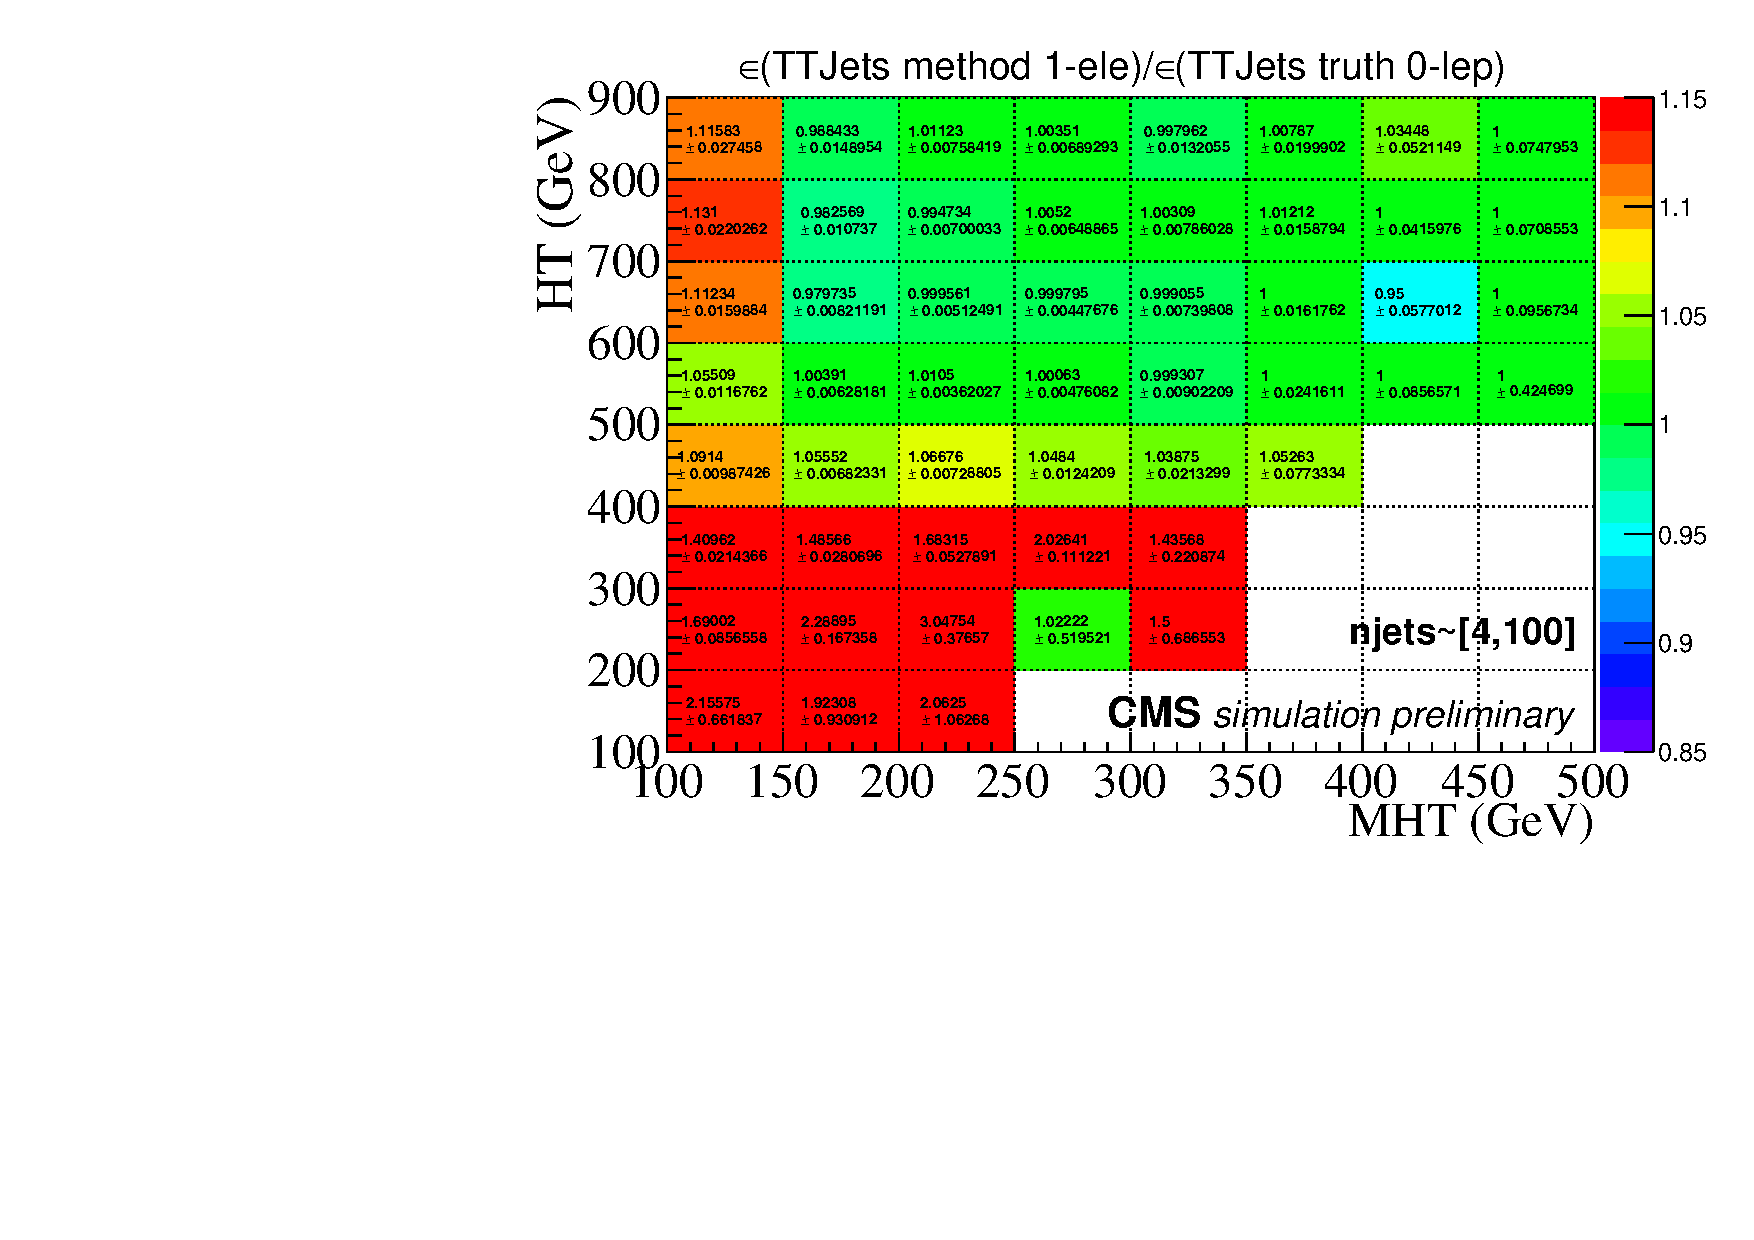
\includegraphics[width=0.95\linewidth]{figures/trigger/EfficiencyRatioMethodTruth.pdf}
    \caption{
      The ratio of the trigger efficiency for events passing the single
      electron reference trigger to the trigger efficiency for all
      events in a simulated $\ttbar$ sample, as a function of the offline $\Ht$
      and $\mht$. The ratio is consistent with 1 within the region of
      the baseline selection of $\Ht>500$ GeV and $\mht>200$ GeV of the CMS hadronic searches.
    }
    \label{fig:2dEffRatio}
  \end{center}
\end{figure}
It is seen that this method, namely, the choice of reference trigger, allows for an unbiased estimate of the trigger efficiency in the region $\mht>150$ GeV and $\Ht>500$, which fortunately includes the baseline selection of the analyses that used this trigger, which impose offline selections of $\mht>200$ GeV and $\Ht>500$ GeV or similar.
These searches, including the multi-jet + $\mht$ search~\cite{Khachatryan:2016kdk}, are briefly summarized in Section \ref{sec:2015results}). 

The efficiency, estimated without bias using Equation \ref{eq:trigeff}, is shown as a function of the offline $\Ht$ and $\mht$, each in 1-dimension, in Fig. \ref{fig:trigger-turnon} using the entire 2015 dataset. 
\begin{figure}[tbp]
  \begin{center}
    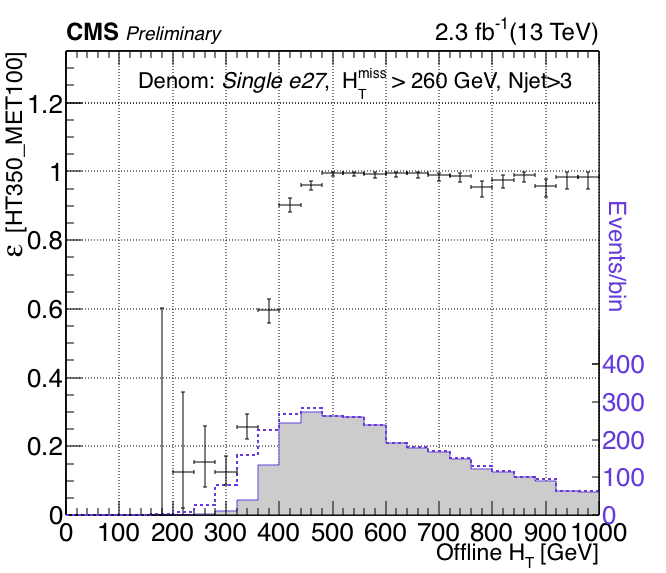
\includegraphics[width=0.49\linewidth]{figures/trigger/EffVsHt2_3InvFb.png}
    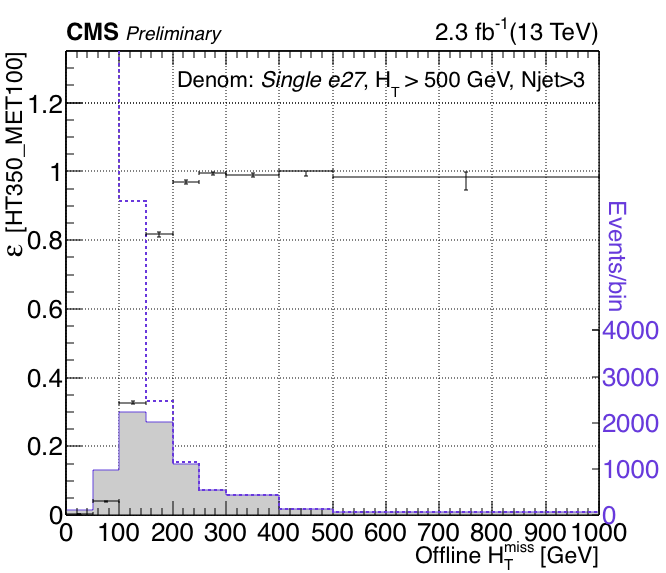
\includegraphics[width=0.49\linewidth]{figures/trigger/EffVsMht2_3InvFb.png}
    \caption{
      The trigger efficiency for \texttt{HLT\_PFHT350\_PFMET100*} 
      as a function of the search variables $\Ht$ and $\mht$. The dashed (solid) blue
      lines show the distributions of the denominator (numerator) samples. These results were used in the CMS PAS on the commissioning of 13 TeV observables for SUSY searches~\cite{CMS-DP-2015-035}.
      }
    \label{fig:trigger-turnon}
  \end{center}
\end{figure}
The statistical uncertainties in the plot are the 68\% CL Clopper-Pearson
intervals~\cite{Clopper:Pearson}. Additionally, a systematic uncertainty is assigned to the efficiency
equal to the difference between the efficiency obtained from applying the method described to a
sample of simulated $\ttbar$ events and that derived
from a set of simulated signal events. Such differences may arise due to any number of subtle differences in the content of the events in $\ttbar$ and signal samples. These uncertainties can be reduced or eliminated by more intelligently choosing a set of observables on which the efficiency estimation depends, in this case the $\Ht$ and $\mht$. This is discussed below under the subsection heading ``Multivariate trigger techniques,'' in the context of more advanced techniques for determining the trigger efficiency. 
\FloatBarrier

\subsubsection{A better trigger: monojet trigger}
There is little reason that the trigger named
\begin{itemize}
  \item \texttt{HLT\_PFMETNoMu90\_PFMHTNoMu90\_*},
\end{itemize}
referred to as the monojet trigger,
was not used in the 2015 multi-jet search. This trigger has no $\Ht$ requirement, and has a lower $\mht$ threshold than that required by the primary trigger. Therefore, the monojet trigger has a higher efficiency in all regions of kinematic phase space, including regions with low $\Ht$ and $\mht$. Furthermore, it is found that, whereas the efficiency estimate for the primary trigger features significant bias in the low $\Ht$ and low $\mht$ regions, indicated by the red portions of the $\Ht-\mht$ plane in Fig. \ref{fig:2dEffRatio}, the equivalent ratio plot for the monojet trigger shows consistency with 1 throughout the entire plane, as seen in Fig. \ref{fig:2dMonoEffRatio}.
\begin{figure}[h]
  \begin{center}
    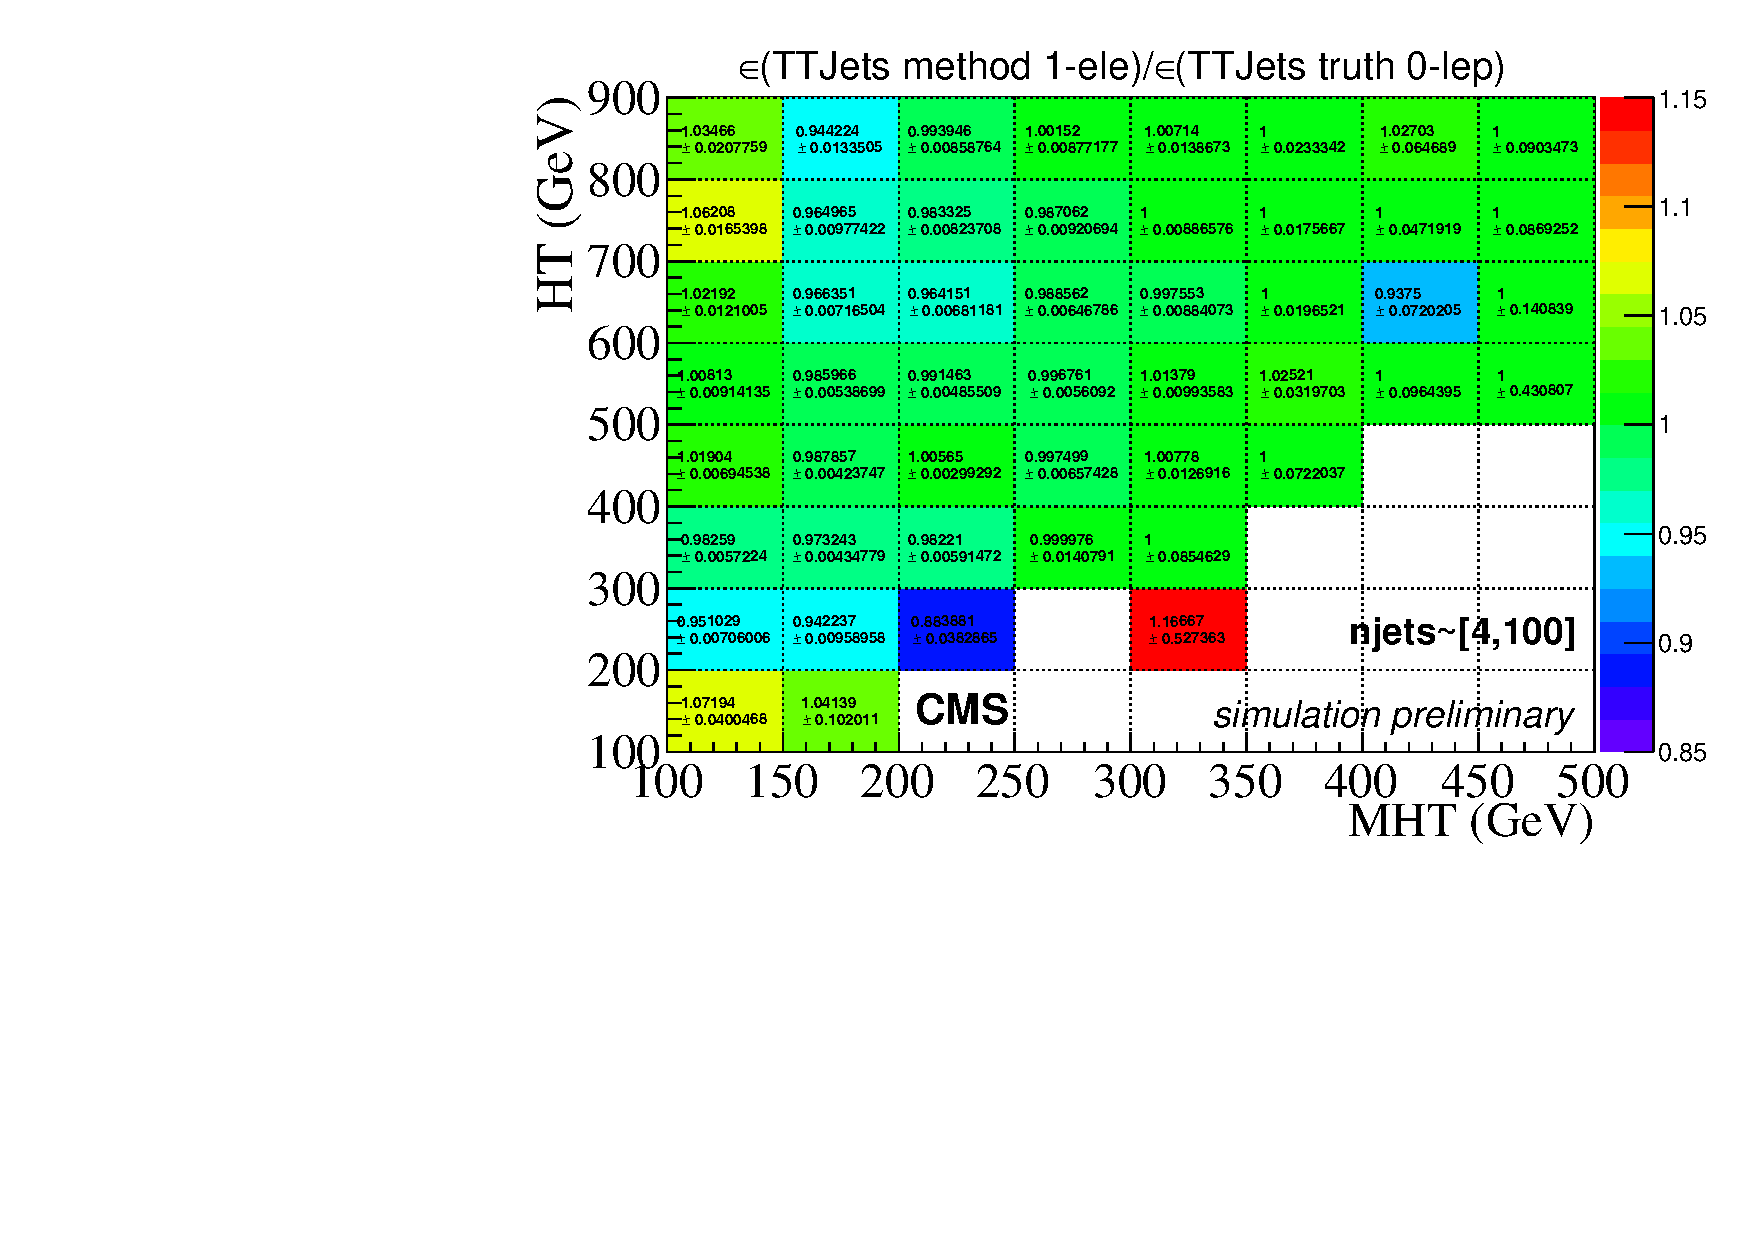
\includegraphics[width=0.95\linewidth]{figures/trigger/MonojetTrigger_EfficiencyRatioMC.pdf}
    \caption{
      The ratio of the monojet trigger efficiency for events passing the single
      electron reference trigger to the trigger efficiency for all
      events in a simulated $\ttbar$ sample, as a function of the offline $\Ht$
      and $\mht$. The ratio is consistent with 1 throughout the $\Ht-\mht$ plane.}
    \label{fig:2dMonoEffRatio}
  \end{center}
\end{figure}
\FloatBarrier
 \noindent
 The monojet trigger is a promising candidate for future analyses that search for evidence of SUSY in the low-$\Ht$ and low-$\mht$ regions, for which it was found that large nonexcluded SUSY cross sections could be manifest in the current data. 
 
\subsubsection{Multivariate efficiency }
\label{sec:mvatrigger}
It is possible for the trigger efficiency to vary as a complicated function of the observables in events. Often, a trigger decision involves a long chain of HLT (Chapter \ref{chap:cms} Section \ref{sec:Trigger}) modules, or filters, that can potentially induce unforeseen dependencies of the probability of firing the trigger on non-trivial correlations among the observables. One way to account for these correlations is to increase the dimensionality of the parametrization of the trigger efficiency estimation. For example, the jet multiplicity could be added as a third dimension to accompany the previously described $\Ht$ and $\mht$ parameterization if it were believed that $\njets$ were a determinant of the efficiency. However, adding additional dimensions requires the division of the event sample into a larger number of bins, which reduces the counts in each bin. This approach is ultimately plagued by the curse of dimensionality.

It is possible to reduce the dimensionality of the parametrization to just 1 dimension by constructing an appropriate single-valued function of the relevant observables. Such a function can be obtained through the use of a Bayesian neural network (NN) classifier, as previously demonstrated by Sezen Sekmen, Wee Don Teo, and Harrison Prosper in the context of b-tagging triggers \cite{bib:SezenTrigger}. 

As stated in Equation \ref{eq:mlp}, the output of such a classifier can be interpreted as
\begin{equation}
\text{NN} = P(\text{s}|\vec{\theta}) = \frac{p(\vec{\theta} | {\rm s})}{p(\vec{\theta} | {\rm s})+p(\vec{\theta} | {\rm b})},
\end{equation}
where $\vec{\theta}$ is a vector of observed quantities, also called the data, and s and b are, respectively, the true and false outcomes\textemdash in this case, the decision made by the trigger whether to fire. Since a NN is capable of training with a vector $\theta$ of arbitrary length, it is worth including any observable that may be relevant for the determination of the efficiency. To train the NN for the monojet trigger efficiency, the single electron reference sample is divided into events that fire the monojet trigger, which serve as the signal training events, and events that fail the monojet trigger, which serve as the background training events. There are several internal NN parameters, which govern aspects of the output such as the responsiveness of the output to small fluctuations in the data. These parameters are assigned gaussian prior probability densities that are broad distributions relative to the likelihood functions, which are highly corrugated. This results in posterior densities for the NN parameters that are dominated by the likelihoods. To obtain an uncertainty in the efficiency estimate, the posterior densities of the NN parameters are randomly sampled, and an ensemble of efficiency estimates are obtained. The mode of the envelope of this ensemble defines the central efficiency estimate, and the uncertainty band taken as the interval that is centered on the mode and contains 68\% of the estimated efficiency values. 

Figure \ref{fig:mvatrigger} shows the dependence of the monojet trigger efficiency on a few kinematic variables, both for the NN-derived efficiency and the efficiency computed in the traditional way. As values of the $\Ht$ are scanned over, the NN efficiency reveals a dependence on correlations between the $\Ht$ and $\mht$. Importantly, this manifests as the loss of efficiency for very high $\Ht$ around $\mht\approx200-300$ GeV.

\begin{figure}[tbp]
  \begin{center}
    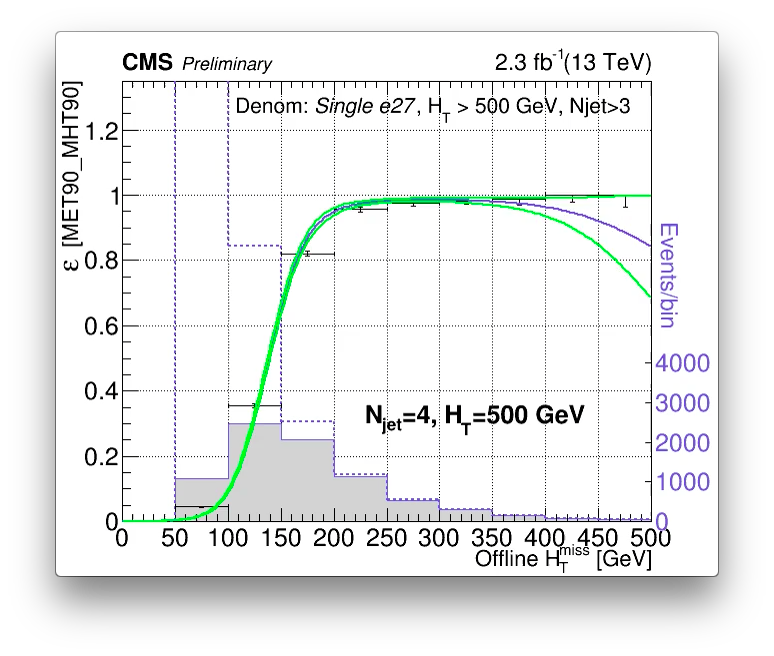
\includegraphics[width=0.49\linewidth]{figures/trigger/MonoTrigEff_Ht500.png}
    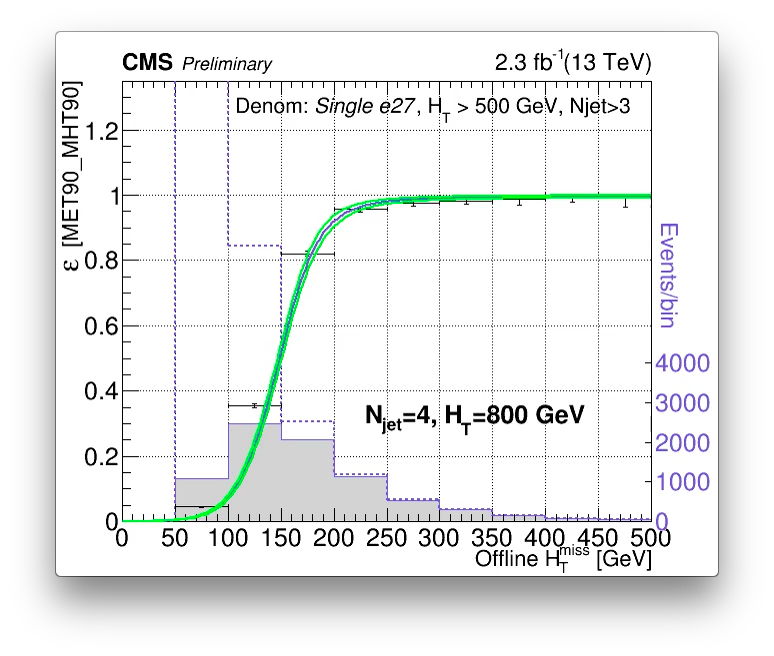
\includegraphics[width=0.49\linewidth]{figures/trigger/MonoTrigEff_Ht800.png}\\
        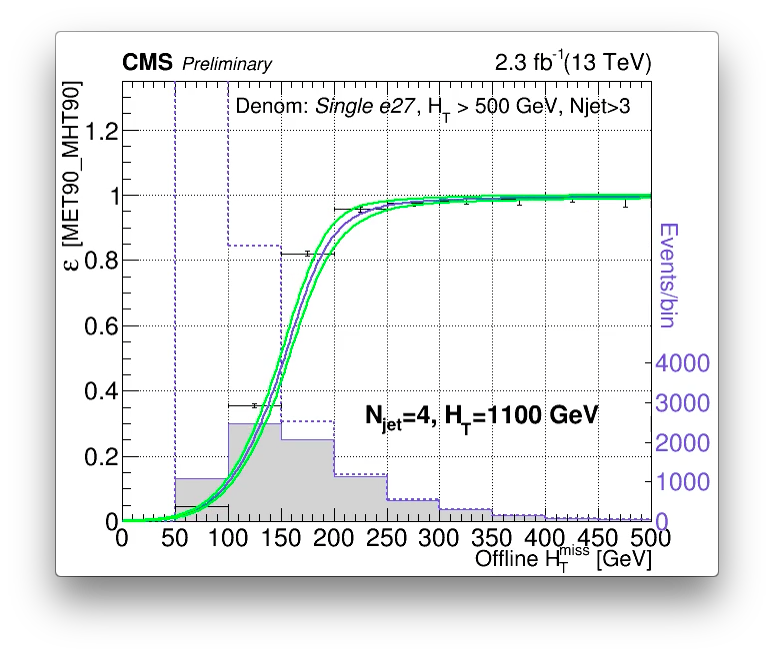
\includegraphics[width=0.49\linewidth]{figures/trigger/MonoTrigEff_Ht1100.png}
    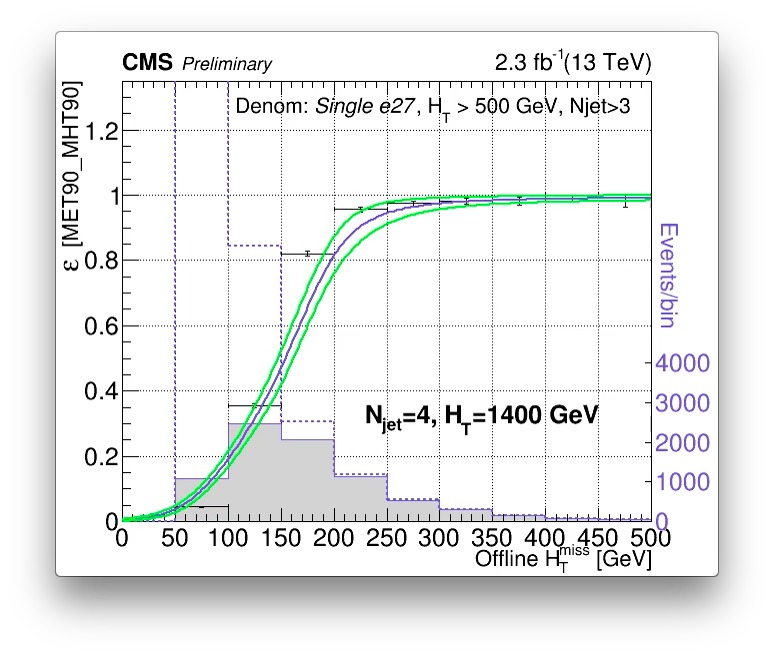
\includegraphics[width=0.49\linewidth]{figures/trigger/MonoTrigEff_Ht1400.png}\\
        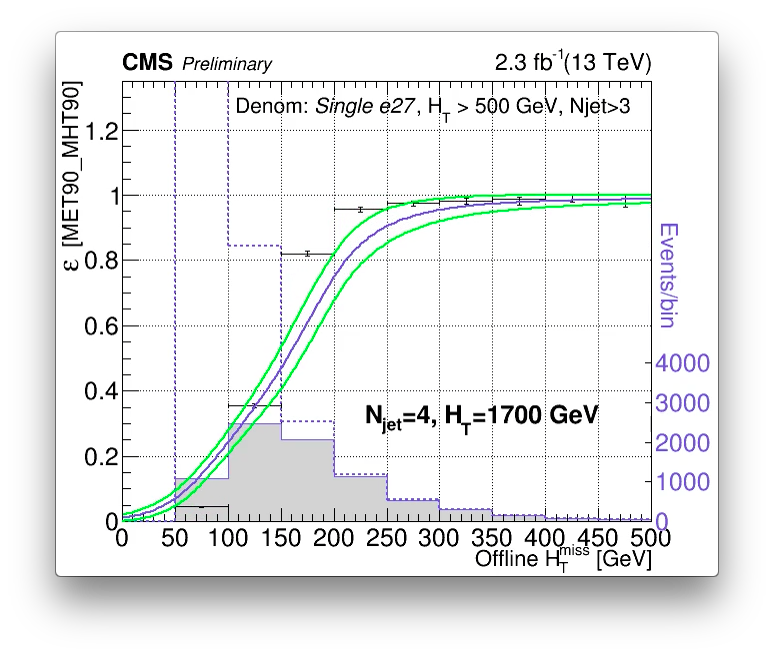
\includegraphics[width=0.49\linewidth]{figures/trigger/MonoTrigEff_Ht1700.png}
    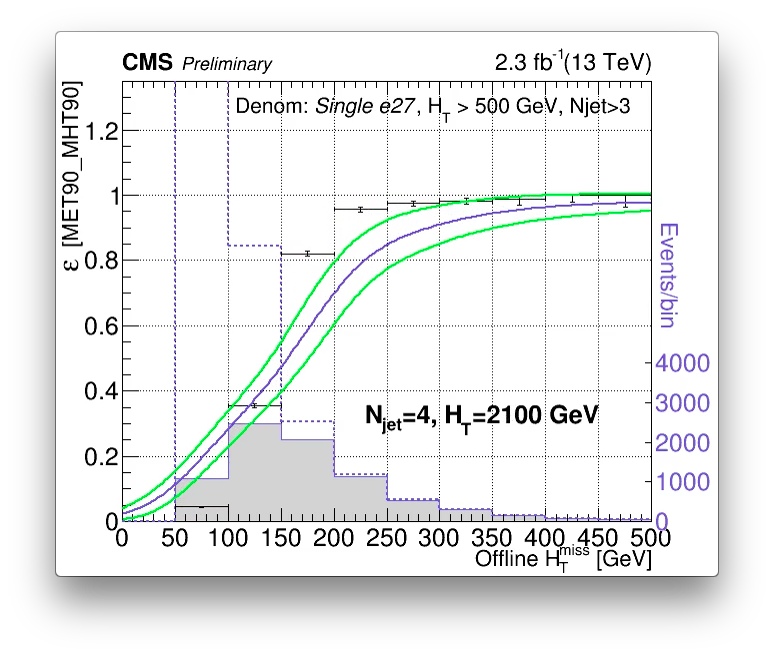
\includegraphics[width=0.49\linewidth]{figures/trigger/MonoTrigEff_Ht2100.png}
    \caption{The trigger efficiency as a function of the offline $\mht$ for the monojet trigger, measured the traditional way (histograms) and by the NN method (blue function), for $\njets=4$, with varying values of the $\Ht$. The green function lines show the 1-sigma uncertainty on the efficiency. }
    \label{fig:mvatrigger}
  \end{center}
\end{figure}
\FloatBarrier
\noindent
This method constitutes a robust model for the trigger that is particularly well-suited for analyses that consider events in regions of kinematic phase space in which the trigger efficiency is varying as a function of the observables.  Typically, analyses, attempt to avoid such regions, since traditional trigger efficiency estimation techniques can hide potentially detrimental effects in these regions, such as the efficiency loss at high $\Ht$ revealed in Fig. \ref{fig:mvatrigger}. Such kinematic regions include the low to moderate $\Ht$ and $\mht$ regions, which were identified as potentially signal rich.


\section{QCD background estimation}
\label{sec:qcd}

Purely hadronic events originating from QCD interactions in proton-proton collisions account for the vast majority of events observed at the LHC. Not surprisingly, these events are a major background to new physics signals that may manifest in the hadronic channel, particularly in regions of low $\met$. Several features of multi-jet QCD events are poorly modeled, including the production cross section, jet multiplicity, and relationships between the directions of jets. This motivates the development of data-driven approaches to QCD estimation. Generally, one takes advantage of the particularly well-modeled aspects of event simulation, but relies on the real data to model as many features as possible. As with any data-driven approach the method must be robust against possible signal contamination that may enter into control regions. 

\subsection{The origin of $\met$ in QCD events}
In order to estimate the QCD background contribution in signal regions with large $\met$, it is relevant to note that the only stable particles in the $\SM$ that are invisible to the CMS detector are neutrinos. Apart from rare final states containing heavy-flavor jets,  QCD events are free of neutrinos, and therefore exhibit little or no $\met$ at the parton level.  For this reason, the $\met$ typically serves as an excellent discriminating variable between the large QCD background and events with significant $\met$, such as models of $R$-parity conserving supersymmetry. However, QCD events {\it only} exhibit zero $\met$ at the parton level $(\met)_{\rm part}$. The final-state particles are detected by a tracker and calorimeters with finite momentum and energy resolution. Mis-measurements of the jet momenta propagate into the measured missing transverse energy, which can result in the measurement of large missing transverse energy, $(\met)_{\rm meas}$, and so QCD events can occupy a similar kinematic region as events predicted by models of new physics.  These statements can be summarized as follows:
\begin{align}
%\begin{split}
(\vec{E}_{ T}^{\rm miss})_{\rm part} &\equiv -\sum_{i=1}^{n}(\vec{p}_{T})_{i,\rm part\ }=0\\
(\vec{E}_{ T}^{\rm miss})_{\rm meas} &\equiv -\sum_{i=1}^{n}(\vec{p}_{T})_{i,\rm meas\ \ \ }\neq 0,
%\end{split}
\label{eq:metTrue}
\end{align}
where $i$ is the particle index and $n$ is the number of particles in the event.

\subsection{Model assumptions and likelihood} 
In general, the magnitudes of the four-vectors of jets at the parton and reconstruction levels differ. However, assuming their directions are identical, the following expression holds for the collection of jets of a given event,
\begin{equation}
\vec{J}_{\rm meas} = \hat{C} \vec{J}_{\rm part},
\end{equation}
where $\vec{J}_{\rm meas}$ and $\vec{J}_{\rm part}$ are $n\times 1$ vectors of the reconstructed jet four-vectors and the parton-level jet four-vectors, and $\hat{C}$ is diagonal $n\times n$ matrix whose elements are the jet energy scale factors $(c_1,c_2,...,c_n)$. The likelihood for a scale factor $c_i\equiv p^{\mu}_{i,\rm meas}/p^{\mu}_{i,\rm part}$, given by
\begin{equation}
L_{i}\equiv{\rm P}(p^{\mu}_{i,\rm meas}|\ p^{\mu}_{i,\rm part})={\rm P}(c_i\ |\ p^{\mu}_{i,\rm part}),
\label{eq:JetEnergyLikelihood}
\end{equation}
is derived from simulation as the distribution of the ratio of reconstruction-level jet momentum to the associated parton-level jet momentum. The association of parton- and reconstruction-level jets is accomplished through the matching criterion,
\begin{equation}
\Delta R(p^{\mu}_{\textrm meas},p^{\mu}_{\textrm parton})<0.4.
\end{equation}	
Additionally, an isolation criterion,
\begin{equation}
p_{\rm T}/\sum_{i=1}^{\njets}[(p_{\rm T})_{i}\cdot\Theta(0.5-\Delta R(p^{\mu}_{i},p^{\mu}))]<1.01,
\end{equation}
is applied both to the parton-level jets and to the reconstruction-level jets that contribute to the likelihood. The jet $\pt$ likelihoods (jet response functions), as shown in Fig. \ref{fig:SmearEx}, are derived in simulation. The likelihoods are measured in 800 finely-spaced bins of parton-level jet $p_T$ and $\eta$.
\begin{figure}[h]
\centering
\subfloat[]{
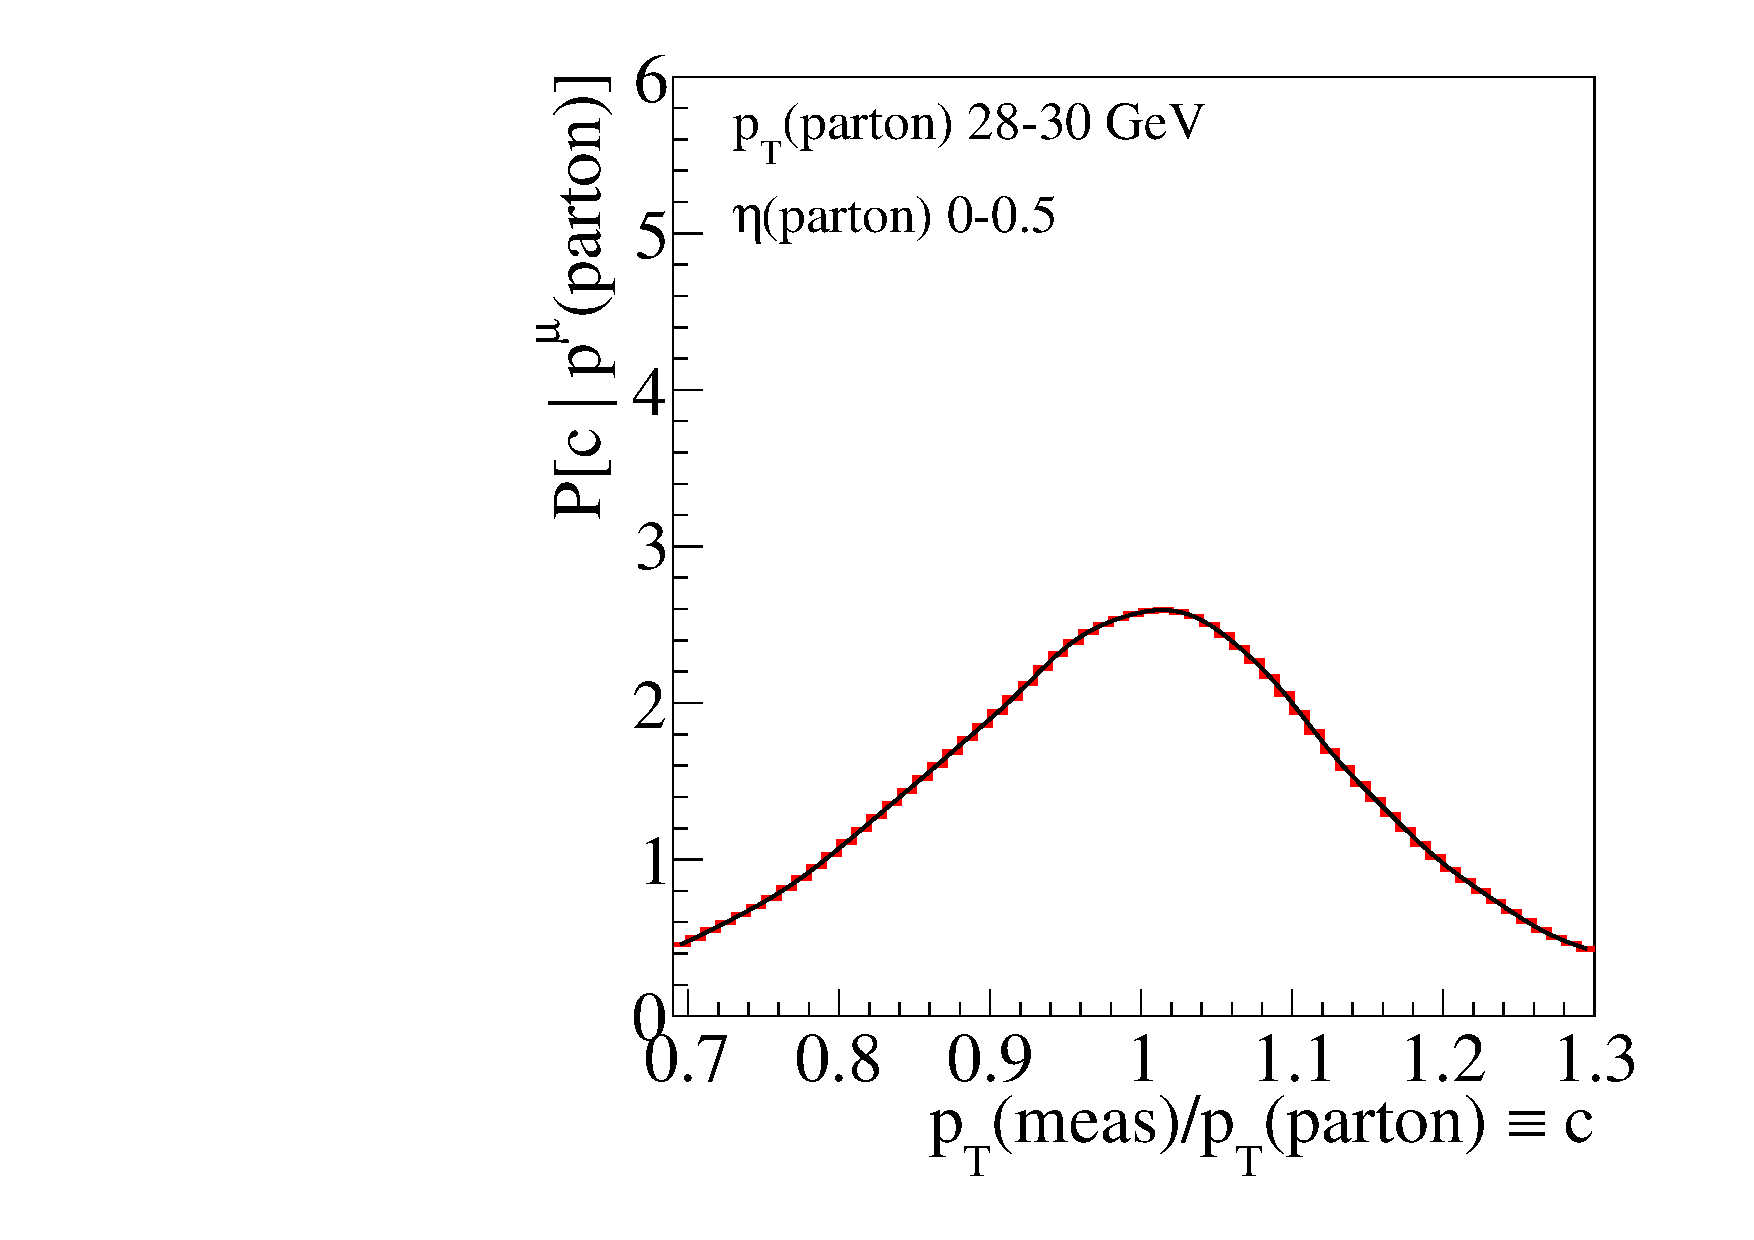
\includegraphics[width=0.5\linewidth]{figures/SusySearches/Ra2b2016/SmearEx1.pdf}
}
\subfloat[]{
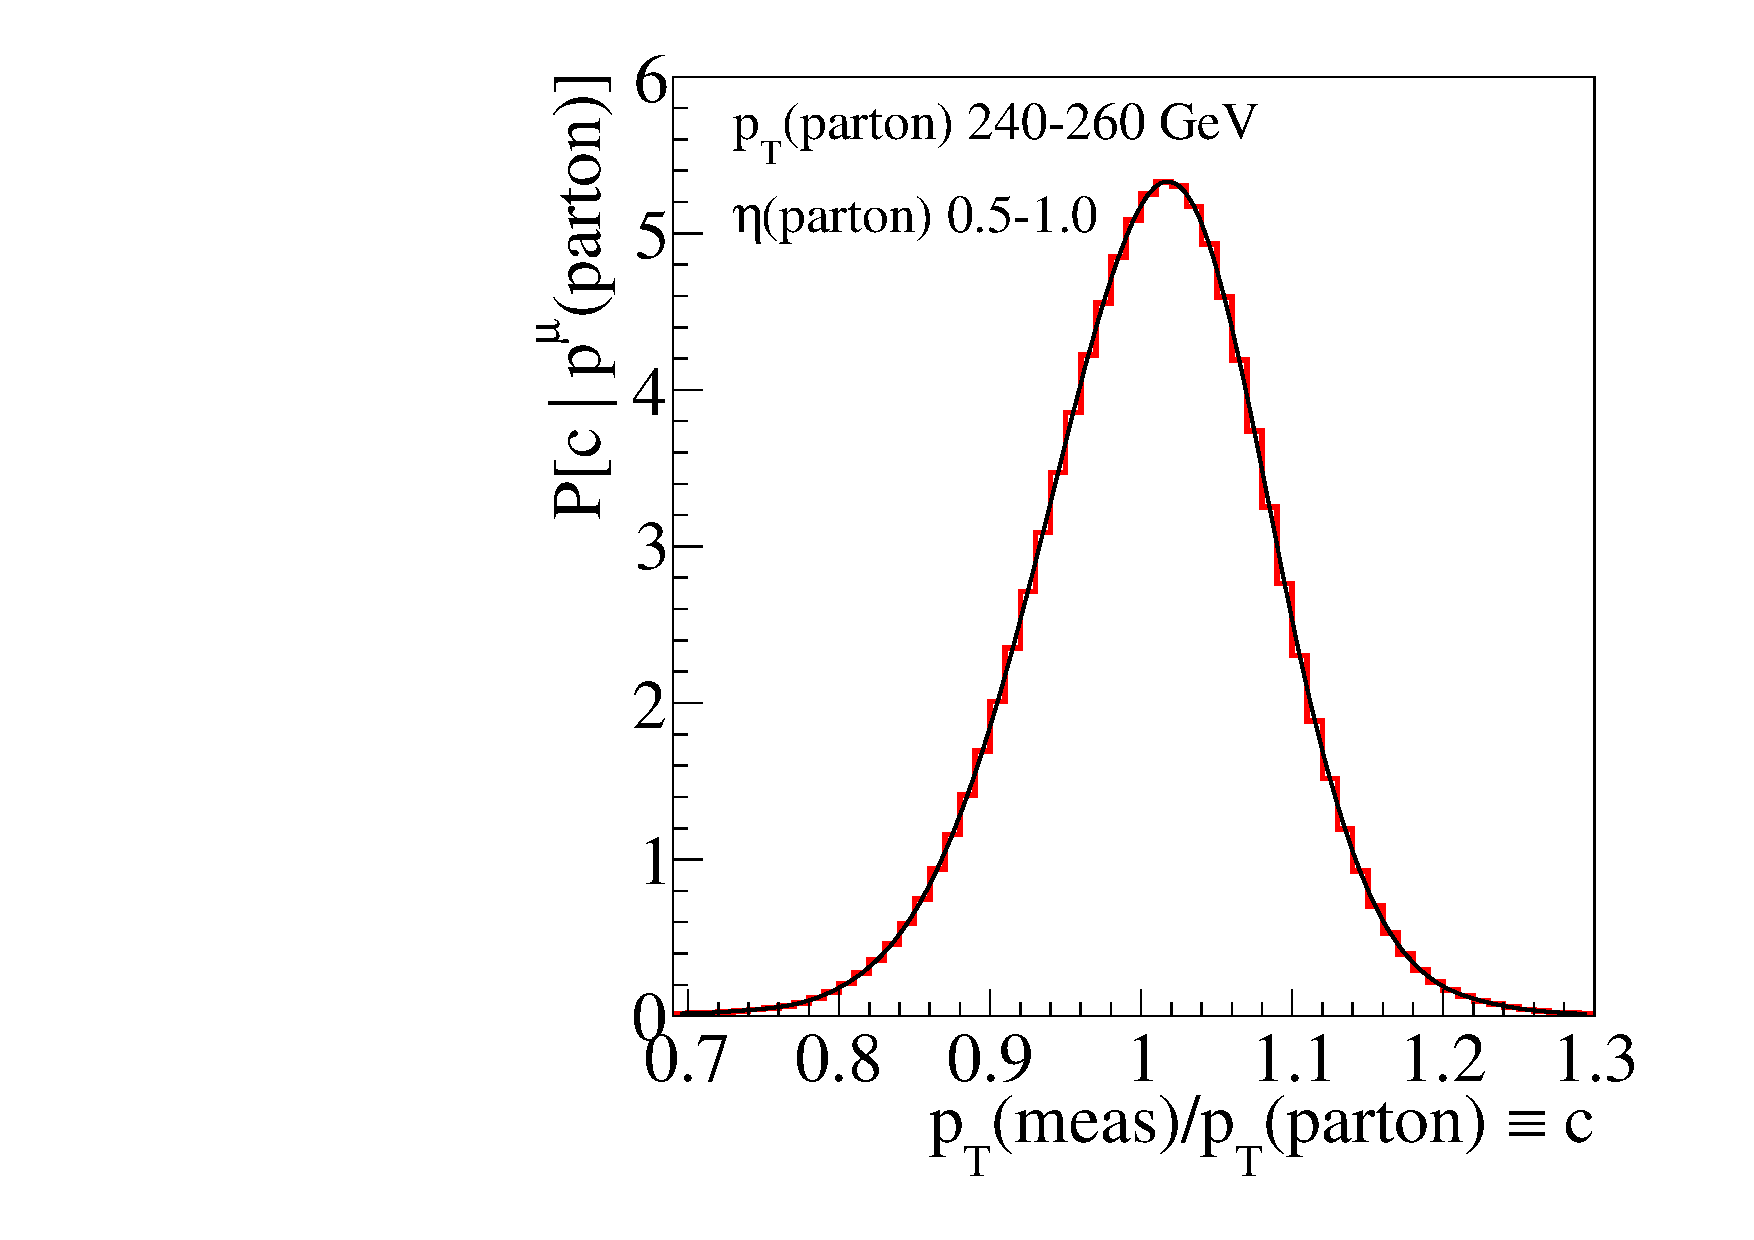
\includegraphics[width=0.5\linewidth]{figures/SusySearches/Ra2b2016/SmearEx2.pdf}
}
\caption{The likelihood function for the jet energy scale factor in two regions of the phase space of the parton-level jet four-vector. These distributions are equivalent to the smearing templates. The histograms (red) are smoothly interpolated using splines (black).}
\label{fig:SmearEx}
\end{figure}


\subsection{Rebalance and smear method}
The rebalance and smear method, originally developed by the authors of the Dissertations~\cite{Koay:2011qqa}\cite{Schroder:2012lqa}\cite{Goebel:2015kca} and the paper~\cite{Chatrchyan:2014lfa}, exploits the relationships given in Equations \ref{eq:metTrue}, along with the jet energy resolution, to form a transfer function between the measured and parton-level jets. The first step of the method is to identify the optimal matrix of scale factors $\hat{C}$ that transforms the collection of reconstruction-level jets into a set that resembles a parton-level jet collection, and (historically) yields an event with $\mht=0$; jets in the resulting collection are referred to as the rebalanced jets. In the second step, the four-vectors of the rebalanced jets are smeared according to the likelihood for the scale factor given in Equation \ref{eq:JetEnergyLikelihood}; events can be smeared as many times as is necessary to make predictions in all signal regions. The above procedure, applied to all events in a QCD-enriched data control sample, yields an event sample that is the basis of the QCD background prediction. Predictions for the QCD background in the signal regions are derived from cuts applied to this sample, which we may refer to as the prediction event sample. I have adapted key aspects of the methodology, which I will now describe step-by-step.

\subsubsection{Rebalance procedure: a Bayesian approach}
The objective is to rebalance the collection of measured jets so that it resembles a parton-level collection. In the re-envisioned approach,  it is possible to systematically  incorporate prior knowledge about the true $\mht$ distribution and jet response functions to constrain the jets.  An inversion of the likelihood function for the jet energy scale factors is performed using Bayes' theorem (see Chapter \ref{chap:run1pmssm} for a brief introduction). The probability density for the parton-level jet collection can be written as
\begin{equation}
{\rm P}(\vec{J}_{\rm part}|\vec{J}_{\rm meas}) \sim {\rm P}(\vec{J}_{\rm meas}|\vec{J}_{\rm part})\cdot \pi(\vec{J}_{\rm part}),
\label{eq:posterior1}
\end{equation}
where $\pi(\vec{J}_{\rm part})$ is the $n$-dimensional prior probability density for the parton-level jet collection.
Treating the jets as mutually independent allows the likelihood to be factorized as
\begin{align}
\begin{split}
{\rm P}(\vec{J}_{\rm meas}|\vec{J}_{\rm part}) = \prod_{i=1}^{\njets}L_{i} &= \prod_{i=1}^{\njets}{\rm P}(p^{\mu}_{i,\rm meas}\ |\ p^{\mu}_{i,\rm part})\\
&=\prod_{i=1}^{\njets}{\rm P}(c_i\ |\ p^{\mu}_{i,\rm part}).
\end{split}
\label{eq:likelihood1}
\end{align}
The prior allows our knowledge about the parton-level missing transverse energy outlined in Equation \ref{eq:metTrue} to constrain the rebalance of the jets. However, while equations \ref{eq:metTrue} are true for the $E_{T}^{\rm miss}$, high pileup conditions necessitate the use of the so-called missing transverse hadronic energy $\mht$, defined as
\begin{equation}
\vec{H}_{T}^{\rm miss} \equiv -\sum_{i=1}^{{\rm N}_{\rm jet}}(\vec{p}_{T})_{i}\cdot\Theta(30{\rm\ GeV}-(p_{T})_{i}).
\end{equation}
The threshold on the $p_{T}$ applied via the Heaviside function to remove jets originating from pileup interactions spoils the equality in Equation \ref{eq:metTrue}. Jets with $p_{T}$ less than 30 GeV can recoil off harder jets, and this produces non-zero true $\mht$. However, the parton-level $\mht$ is still small compared to the reconstruction-level $\mht$, as seen in the distribution of parton- and reconstruction-level $\mht$ in Fig. \ref{fig:Mht}, implying that the underlying $\mht$ distribution may provide a meaningful constraint on our knowledge of the parton-level system. A difference is also seen in the angular distribution of the $\mht$, in the polar coordinate system with the z-axis defined along the direction of the leading jet, and this information can likewise be incorporated, as will now be demonstrated.
\begin{figure}[h]
\centering
\subfloat[]{
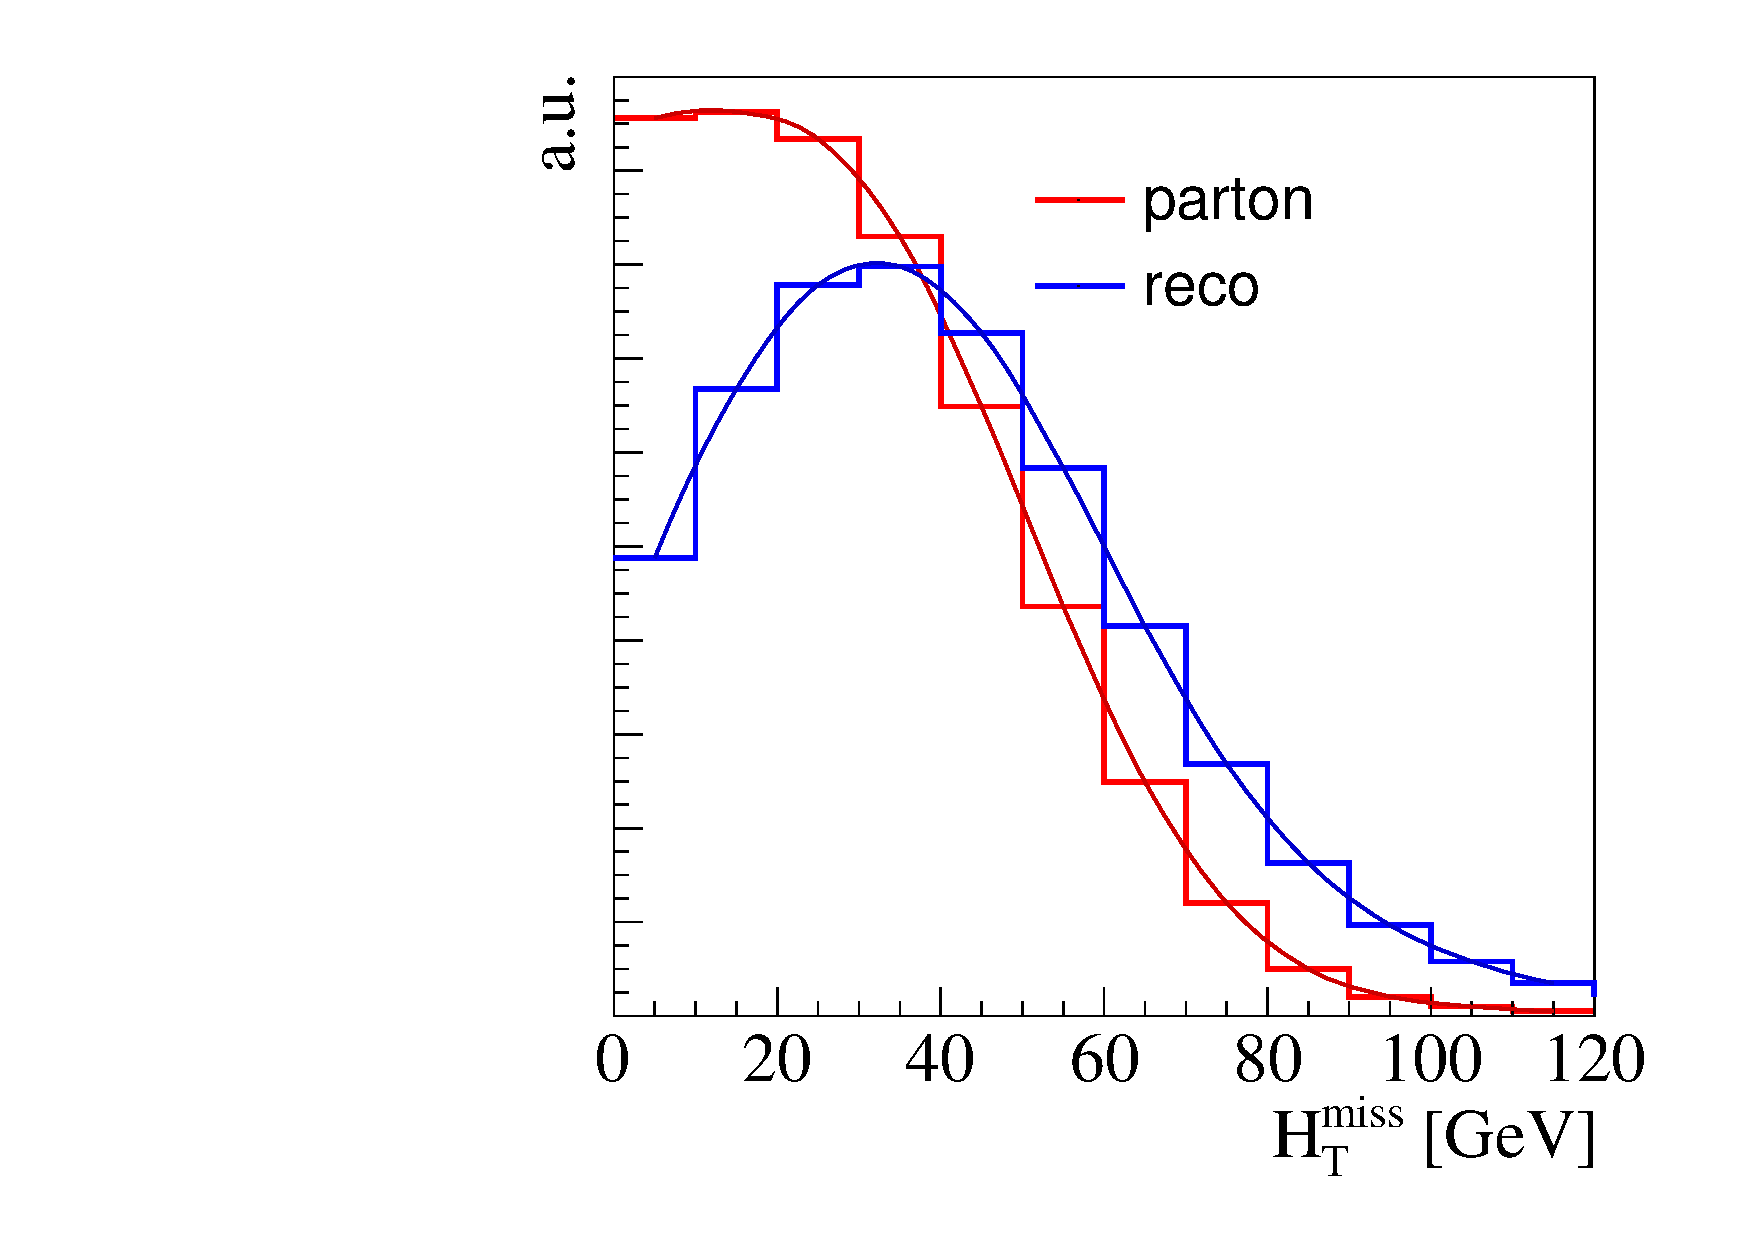
\includegraphics[width=0.5\linewidth]{figures/SusySearches/Ra2b2016/MhtGenAndTruth.pdf}
}
\subfloat[]{
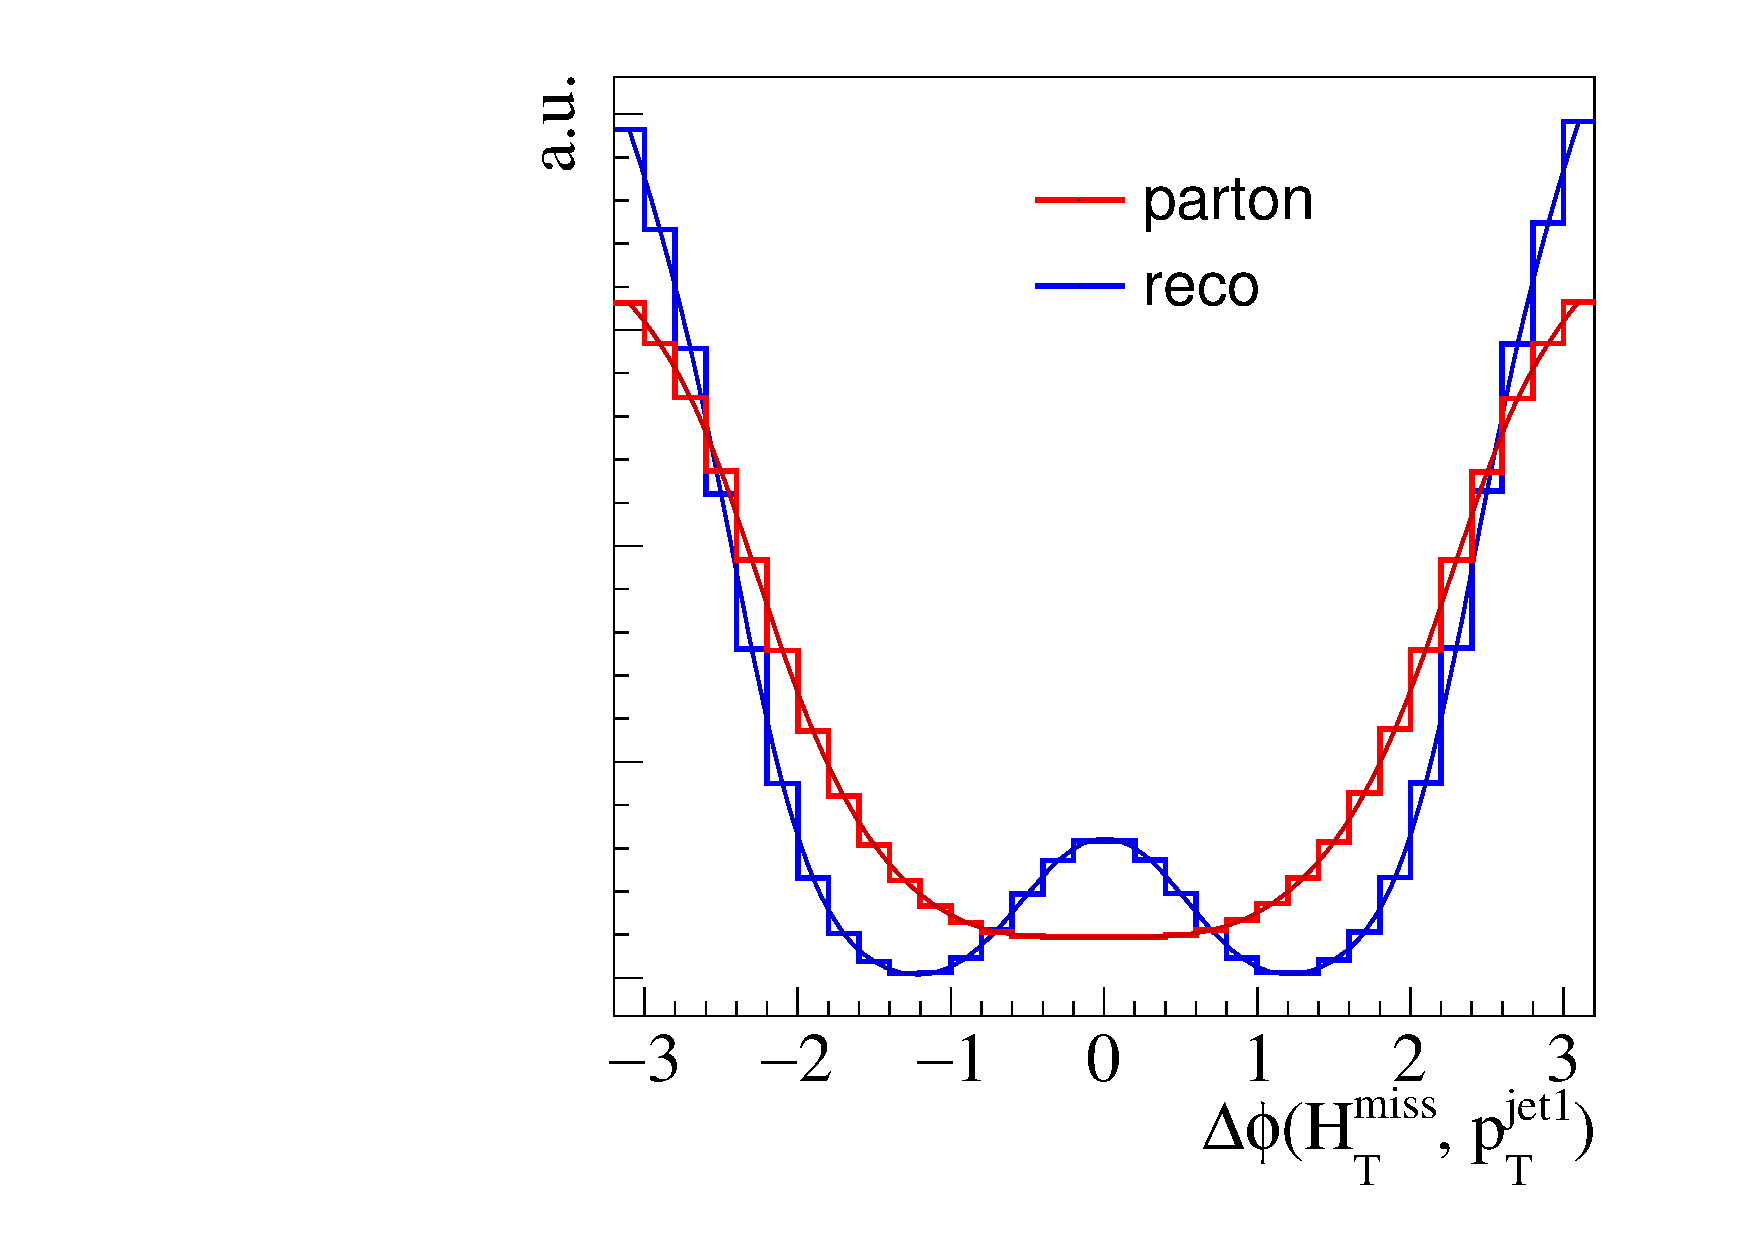
\includegraphics[width=0.5\linewidth]{figures/SusySearches/Ra2b2016/DPhiMhtJet1GenAndTruth.pdf}
}
\caption{The parton-level and reconstruction-level $\mht$ and azimuthal separation between the $\mht$ and leading jet in QCD simulation. The red functions are taken as probability distributions making up the prior, $\text{P}[\mht(\vec{J}_{\rm part})]$ and $\text{P}[\Delta\phi_{\mht,p_{T}^1}(\vec{J}_{\rm part})]$}
\label{fig:Mht}
\end{figure}

The expression relating the parton-level $\mht$ to the jet energy scale factors can be used, in conjunction with the red probability densities, to form factors in the prior. The templates for the $\Delta\phi$ between the $\mht$ and the leading jet are derived separately in bins of the b-jet multiplicity, for the bins of 0, 1, and $\geq$ 2 b-jets.  This choice and its implications are discussed later. For the case of one or more b-jets, the $\Delta\phi$ between the $\mht$ and the leading b-jet is used. Combining Eqs. \ref{eq:posterior1} and \ref{eq:likelihood1} gives
\begin{equation}
{\rm P}(\vec{J}_{\rm part}|\vec{J}_{\rm meas}) \sim
\prod_{i=1}^{\njets}{\rm P}(p^{\mu}_{i,\rm meas}|p^{\mu}_{i,\rm part})\cdot \text{P}[\mht(\vec{J}_{\rm part})]\cdot \text{P}[\Delta\phi_{\mht,p_{T}^1}(\vec{J}_{\rm part})]\cdot \pi_0(\vec{J}_{\rm part}),
\end{equation}
where $\pi_0(\vec{J}_{\rm part})$ is the initial prior on the parton jet four-vectors, taken to be uniform. Having constructed a posterior density, the parton-level jets can be inferred by integrating with respect to the reconstruction-level jet four-vectors, or alternatively, by performing a likelihood maximization. The second approach is taken.


\subsubsection{Posterior density of jet momenta}
Bayes' theorem suggests that incorporating new relevant information will lead to improved knowledge about a system. In the case of the rebalance and smear method, we might expect a rebalanced event to more closely resemble the parton-level event than does the reconstruction-level event. Figure \ref{fig:rebareso} shows that the resolution of rebalanced jets is better than that of reconstructed jets by approximately 10\%.
\begin{figure}[h]
\centering
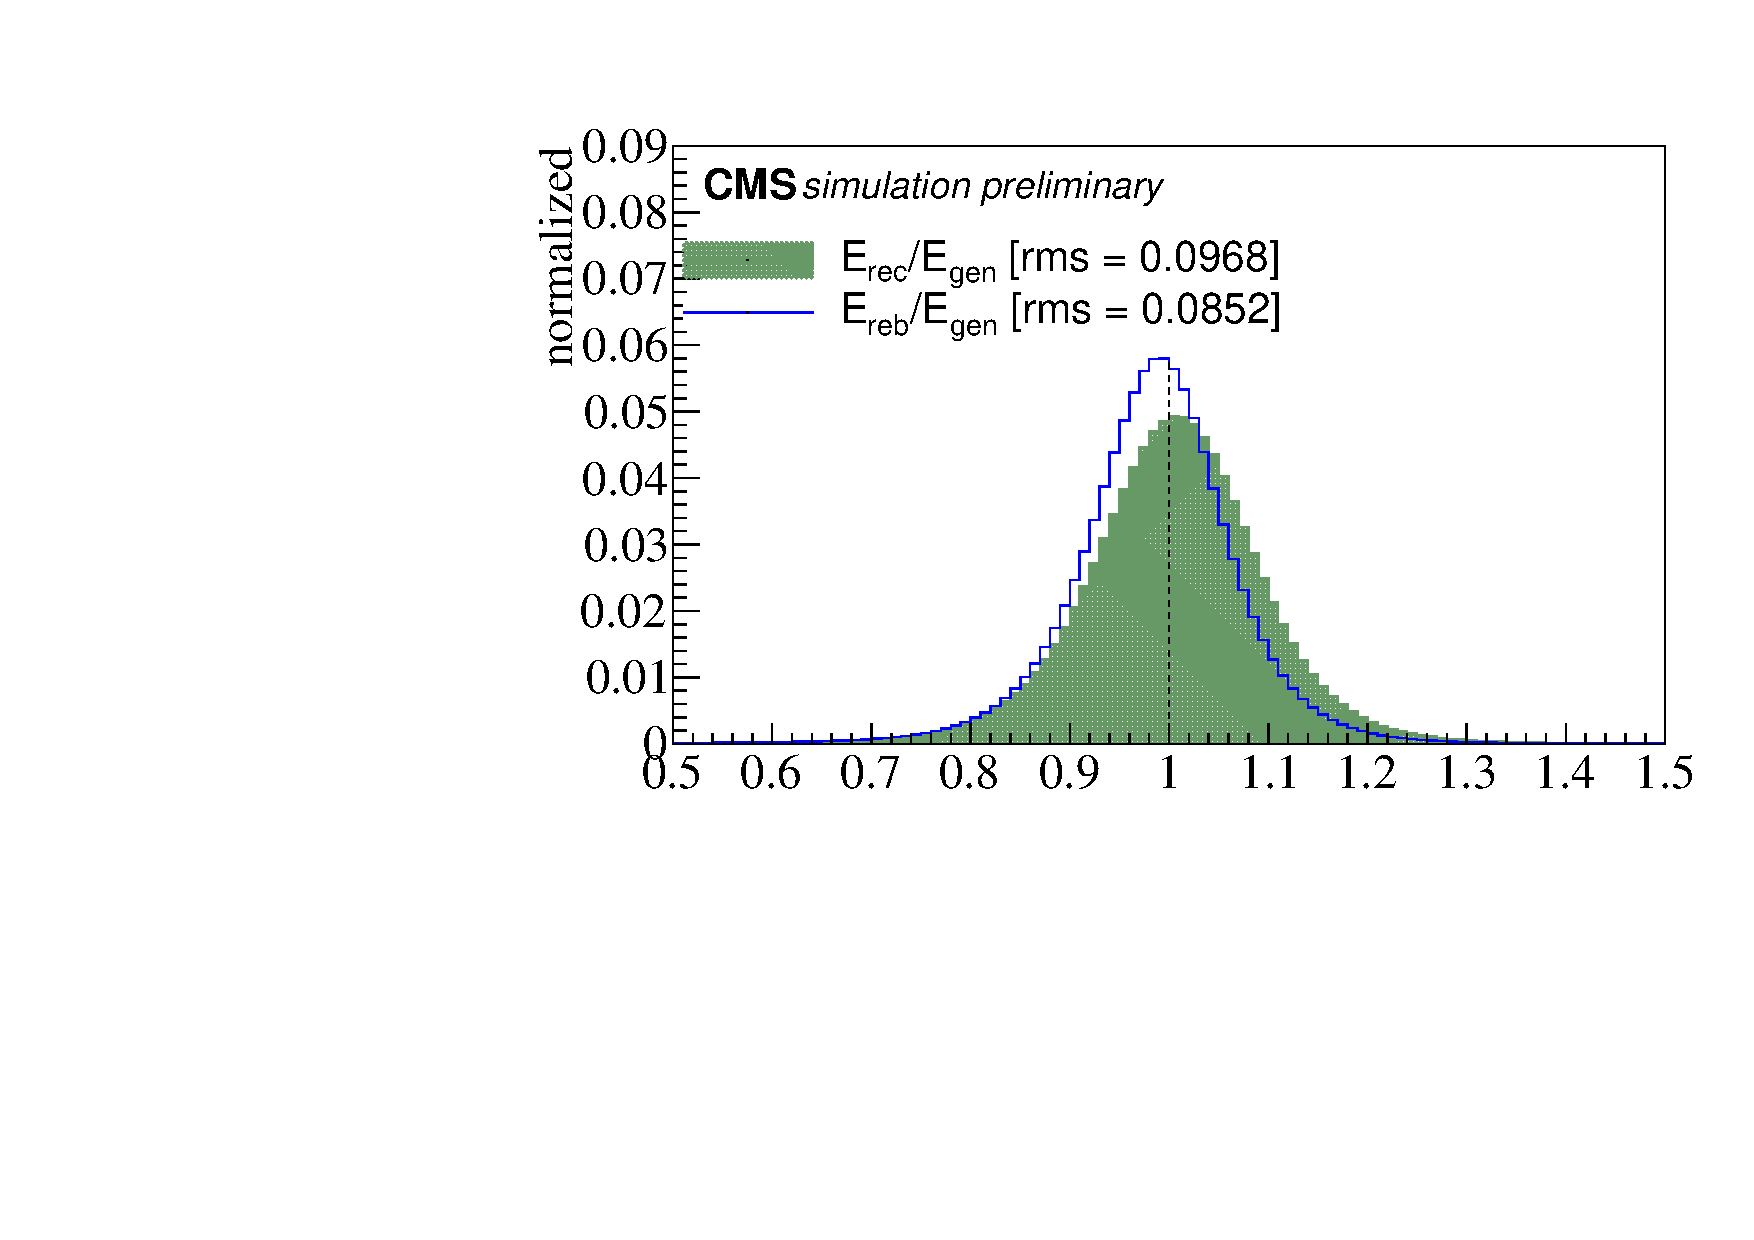
\includegraphics[width=0.49\linewidth]{figures/SusySearches/Ra2b2016/Jet1Resolution.pdf}
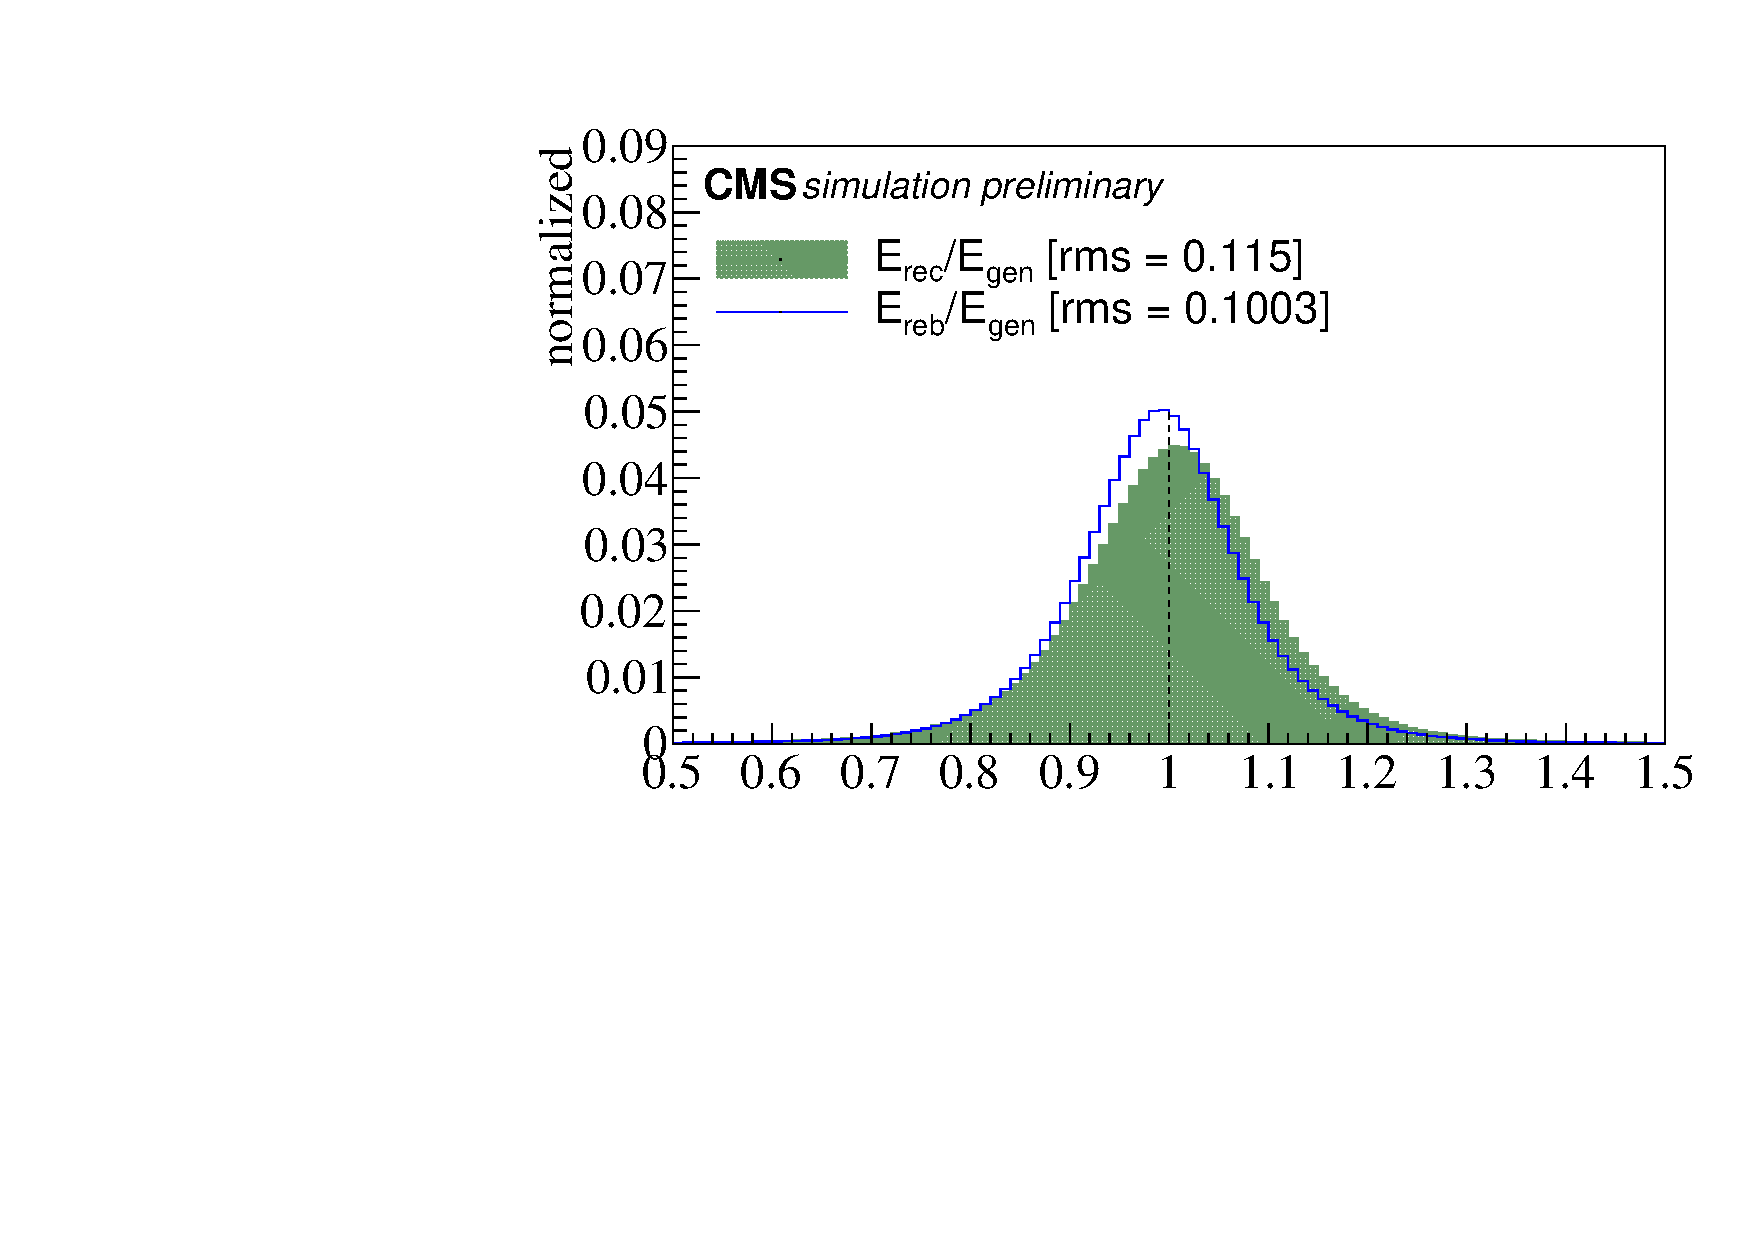
\includegraphics[width=0.49\linewidth]{figures/SusySearches/Ra2b2016/Jet2Resolution.pdf}
\caption{The jet energy response for the leading jet (left) and sub-leading jet (right) for reconstructed jets (green) and rebalanced jets (blue). Parton-level jets are required to have $\pt>30$ GeV and $|\eta|<2.4$. The resolution of rebalanced jets is better (smaller) than that of reconstruction-level jets by bout 10\%.}
\label{fig:rebareso}
\end{figure}
We also observe the peak of the response to be slightly lower for rebalanced jets than for reconstructed jets. This is consistent with the peak of the jet $\pt$ likelihood functions being centered at values slightly higher than 1, as seen in Fig. \ref{fig:SmearEx}. 
\FloatBarrier

\subsection{Closure}
The rebalance and smear prediction is applied to simulated events and compared with the result obtained directly from the simulation. A baseline selection, similar to that applied in the search \cite{Khachatryan:2016kdk}, is applied. Events are required to have:
\begin{itemize}
\item no reconstructed, isolated particle track with a $\pt>10$ GeV and $|\eta|<2.4$;
\item $\Ht>500$ GeV;
\item $\mht>150$ GeV;
\item $\njets\geq$ 4, where jets are required to have a $\pt>30$ GeV and $|\eta|<2.4$, and pass a loose set of quality selection criteria.
\item an azimuthal separation between the $\mht$ and the leading four jets $\Delta\phi(\mht$, jet$_{1,2,3,4})>$ 0.5, 0.5, 0.3, 0.3.
\end{itemize}
Figures \ref{fig:BaselineRplusS} through \ref{fig:BaselineRplusS2} show this comparison for a number of observables after the baseline selection of the CMS multi-jet SUSY search, which is described in Section \ref{sec:2015results}. The distributions are ``n-1'' distributions, meaning all baseline selection have been applied except that of the x-axis variable. Then, Figs. \ref{fig:LowDeltaPhiRplusS} through \ref{fig:LowDeltaPhiRplusS2} show the comparison in the so-called inverted $\Delta \phi$ region, which has a selection equivalent to the baseline, but with the inverse of the selection on the $\Delta \phi$ between the $\mht$ and the jets. Figure \ref{fig:RplusSCorrelation} shows the comparison in two dimensions for selected pairs of observables. 

\begin{figure}[h]
\centering
\subfloat[]{
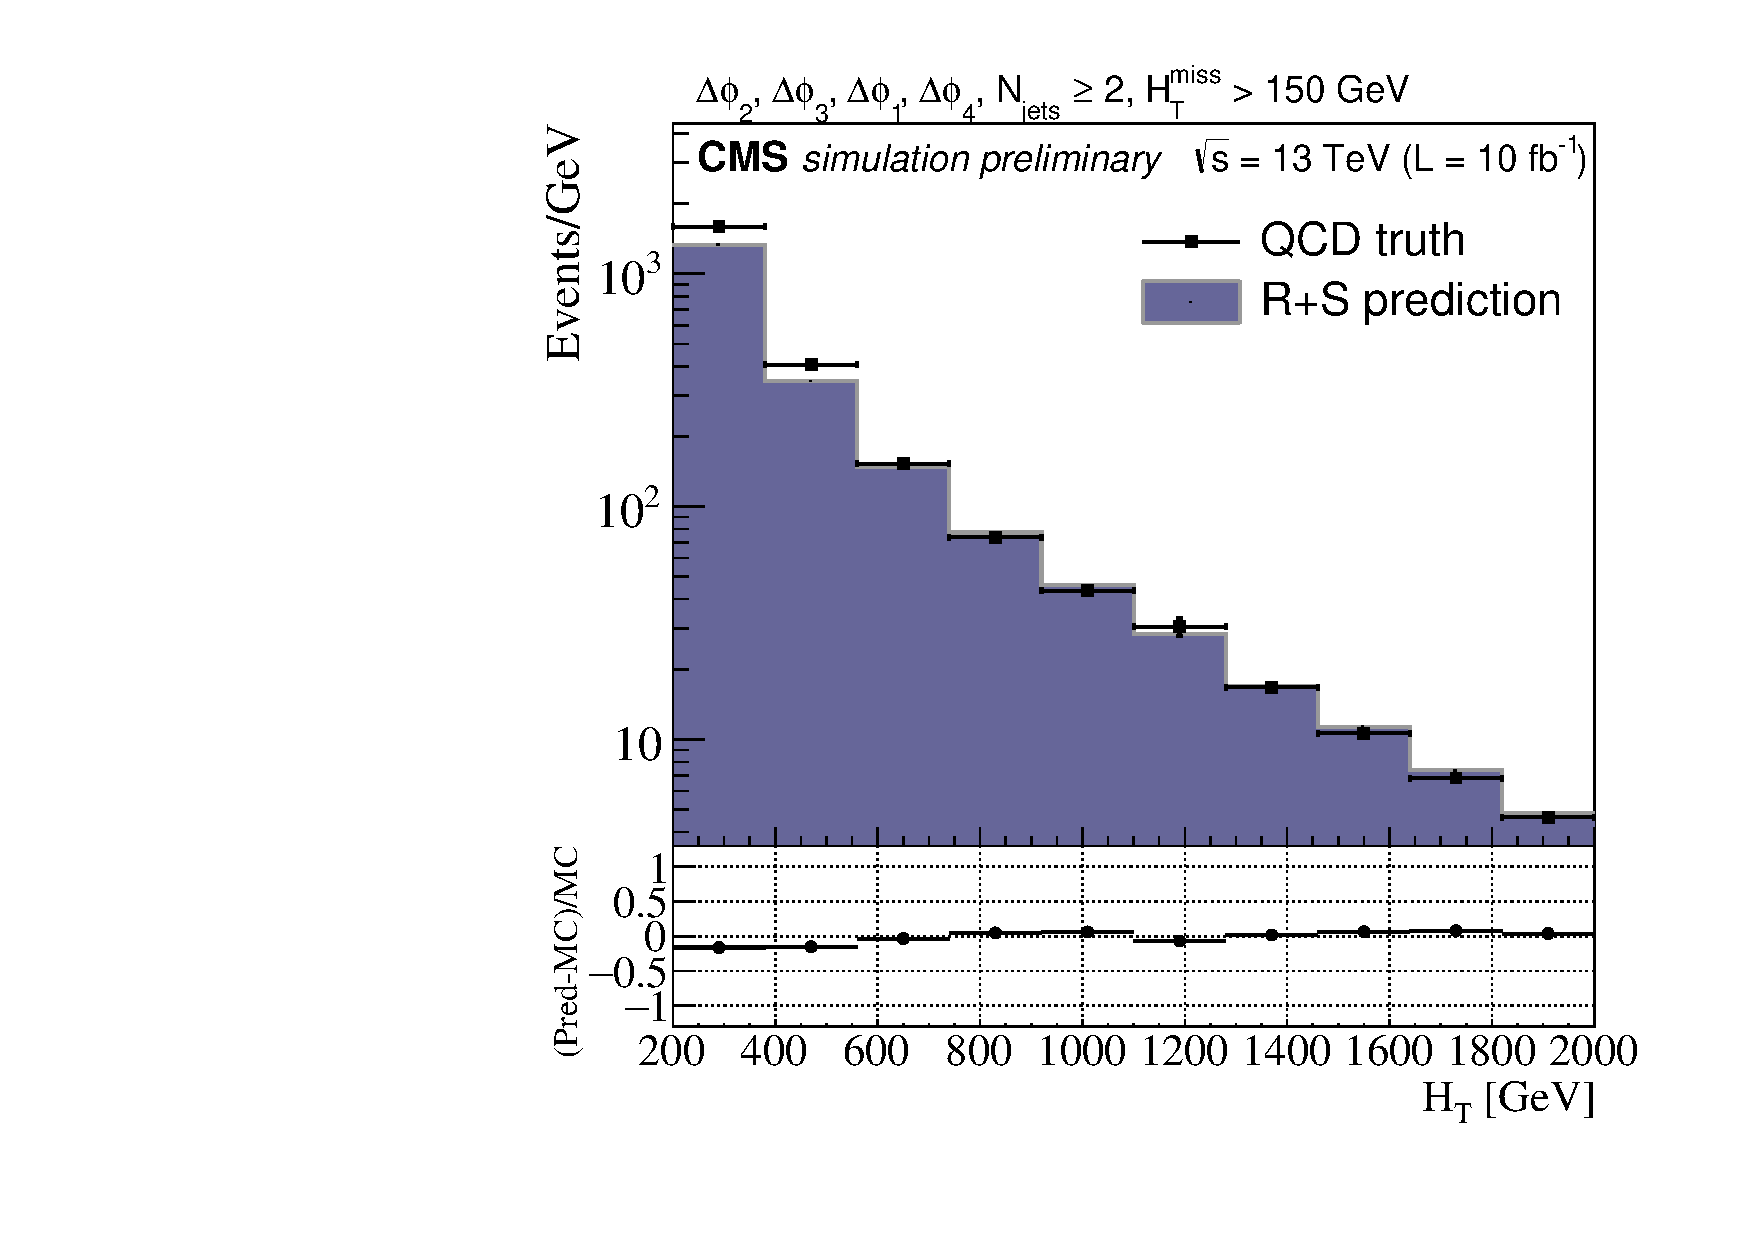
\includegraphics[width=0.5\linewidth]{figures/SusySearches/Ra2b2016/Baseline_Ht.pdf}
}
\subfloat[]{
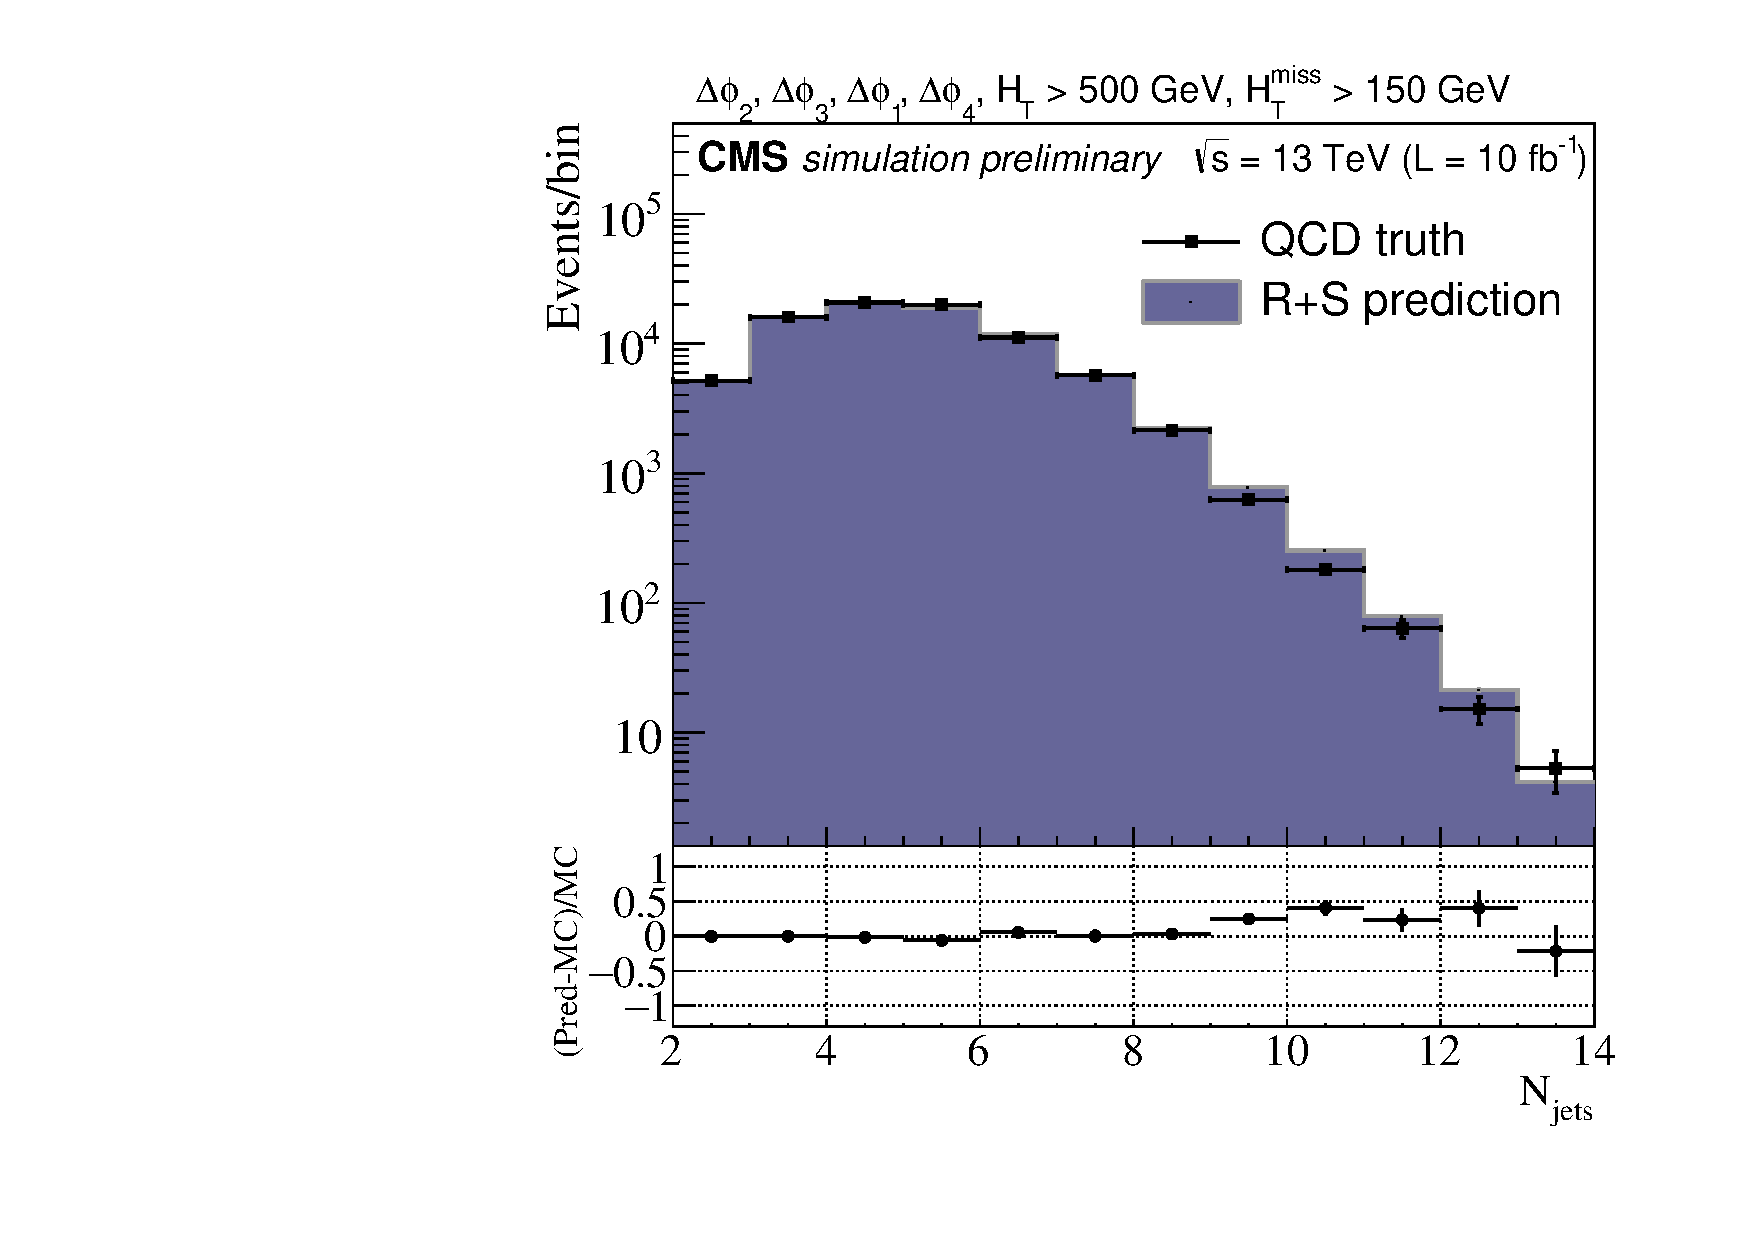
\includegraphics[width=0.5\linewidth]{figures/SusySearches/Ra2b2016/Baseline_NJets.pdf}
}\\
\subfloat[]{
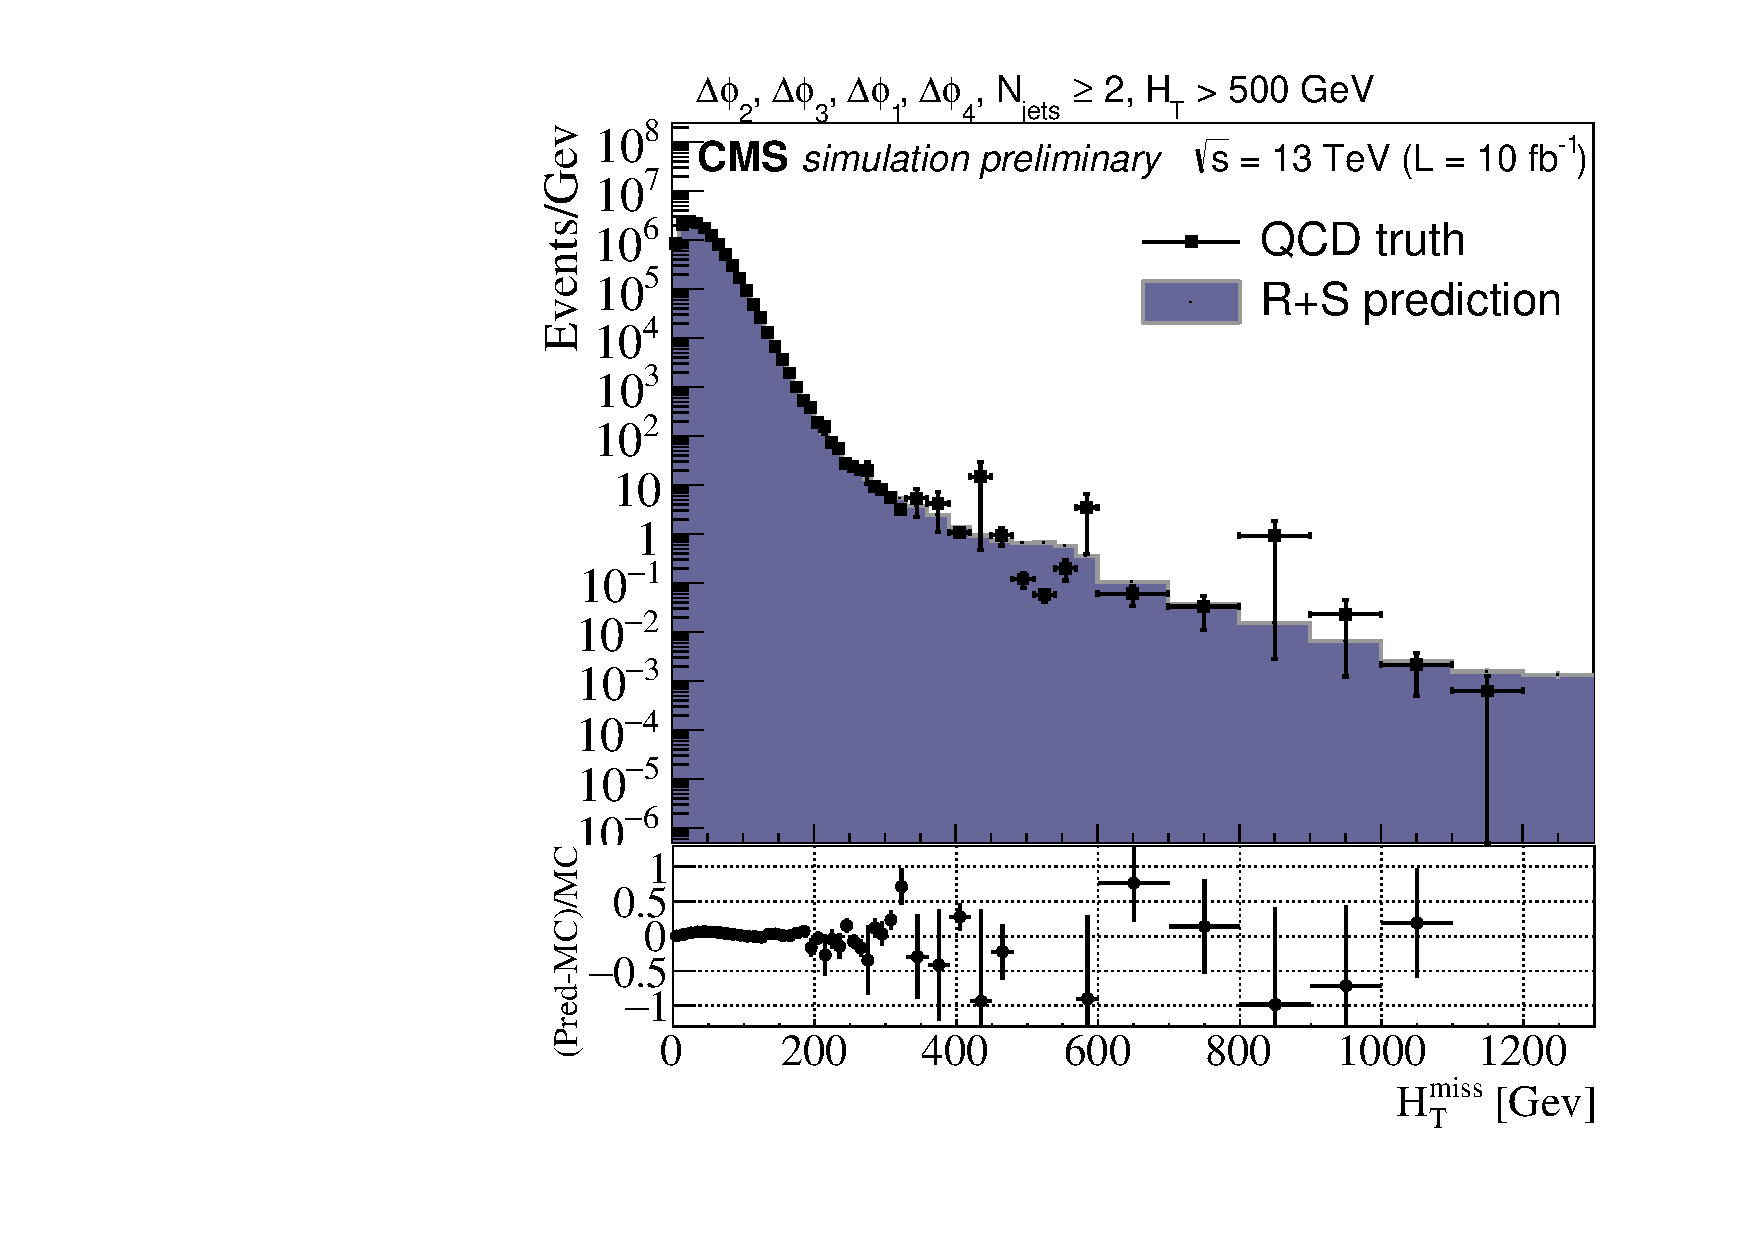
\includegraphics[width=0.5\linewidth]{figures/SusySearches/Ra2b2016/Baseline_Mht.pdf}
}
\subfloat[]{
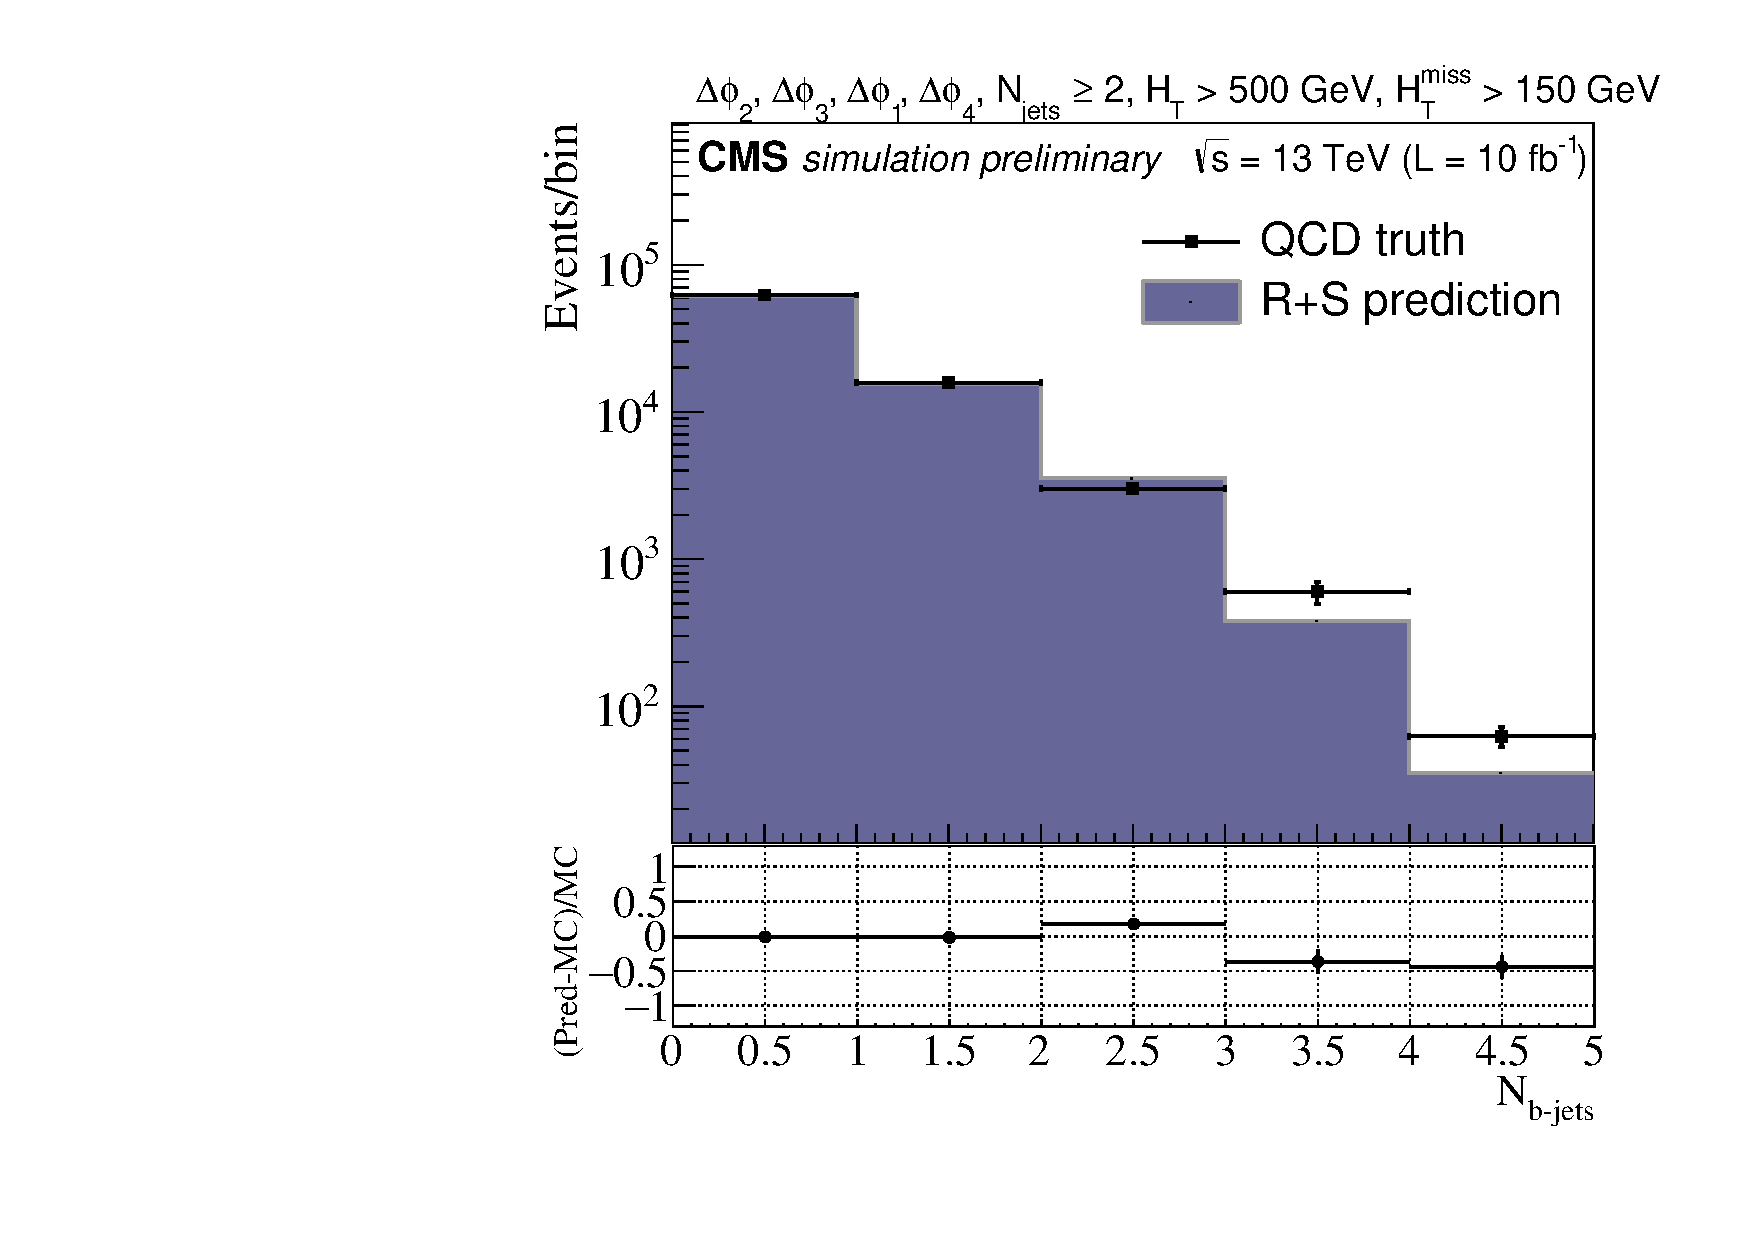
\includegraphics[width=0.5\linewidth]{figures/SusySearches/Ra2b2016/Baseline_BTags.pdf}
}
\caption{Comparisons of kinematic distributions between the direct simulation and the rebalance and smear method applied to simulation, after the baseline selection of the multi-jet SUSY search.}
\label{fig:BaselineRplusS}
\end{figure}


\begin{figure}[h]
\centering
\subfloat[]{
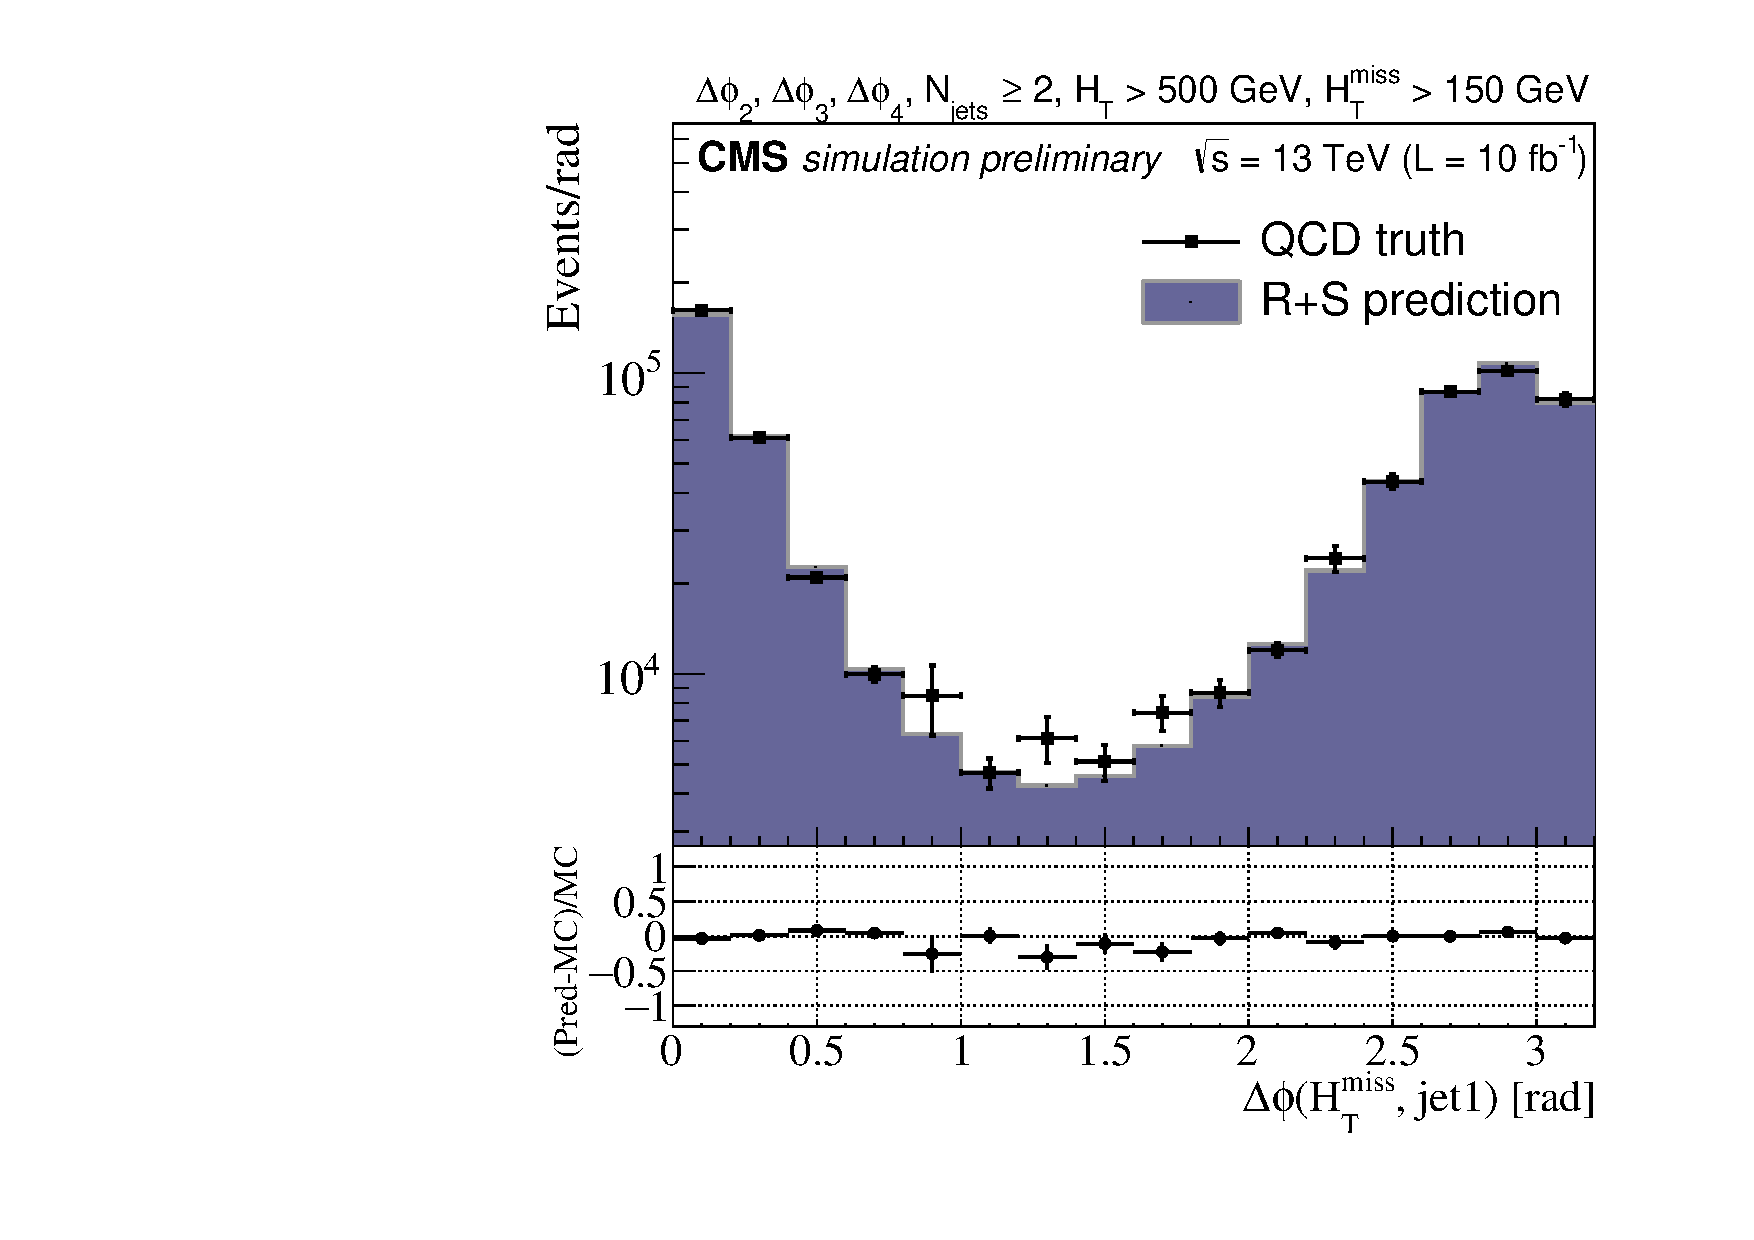
\includegraphics[width=0.5\linewidth]{figures/SusySearches/Ra2b2016/Baseline_DPhi1.pdf}
}
\subfloat[]{
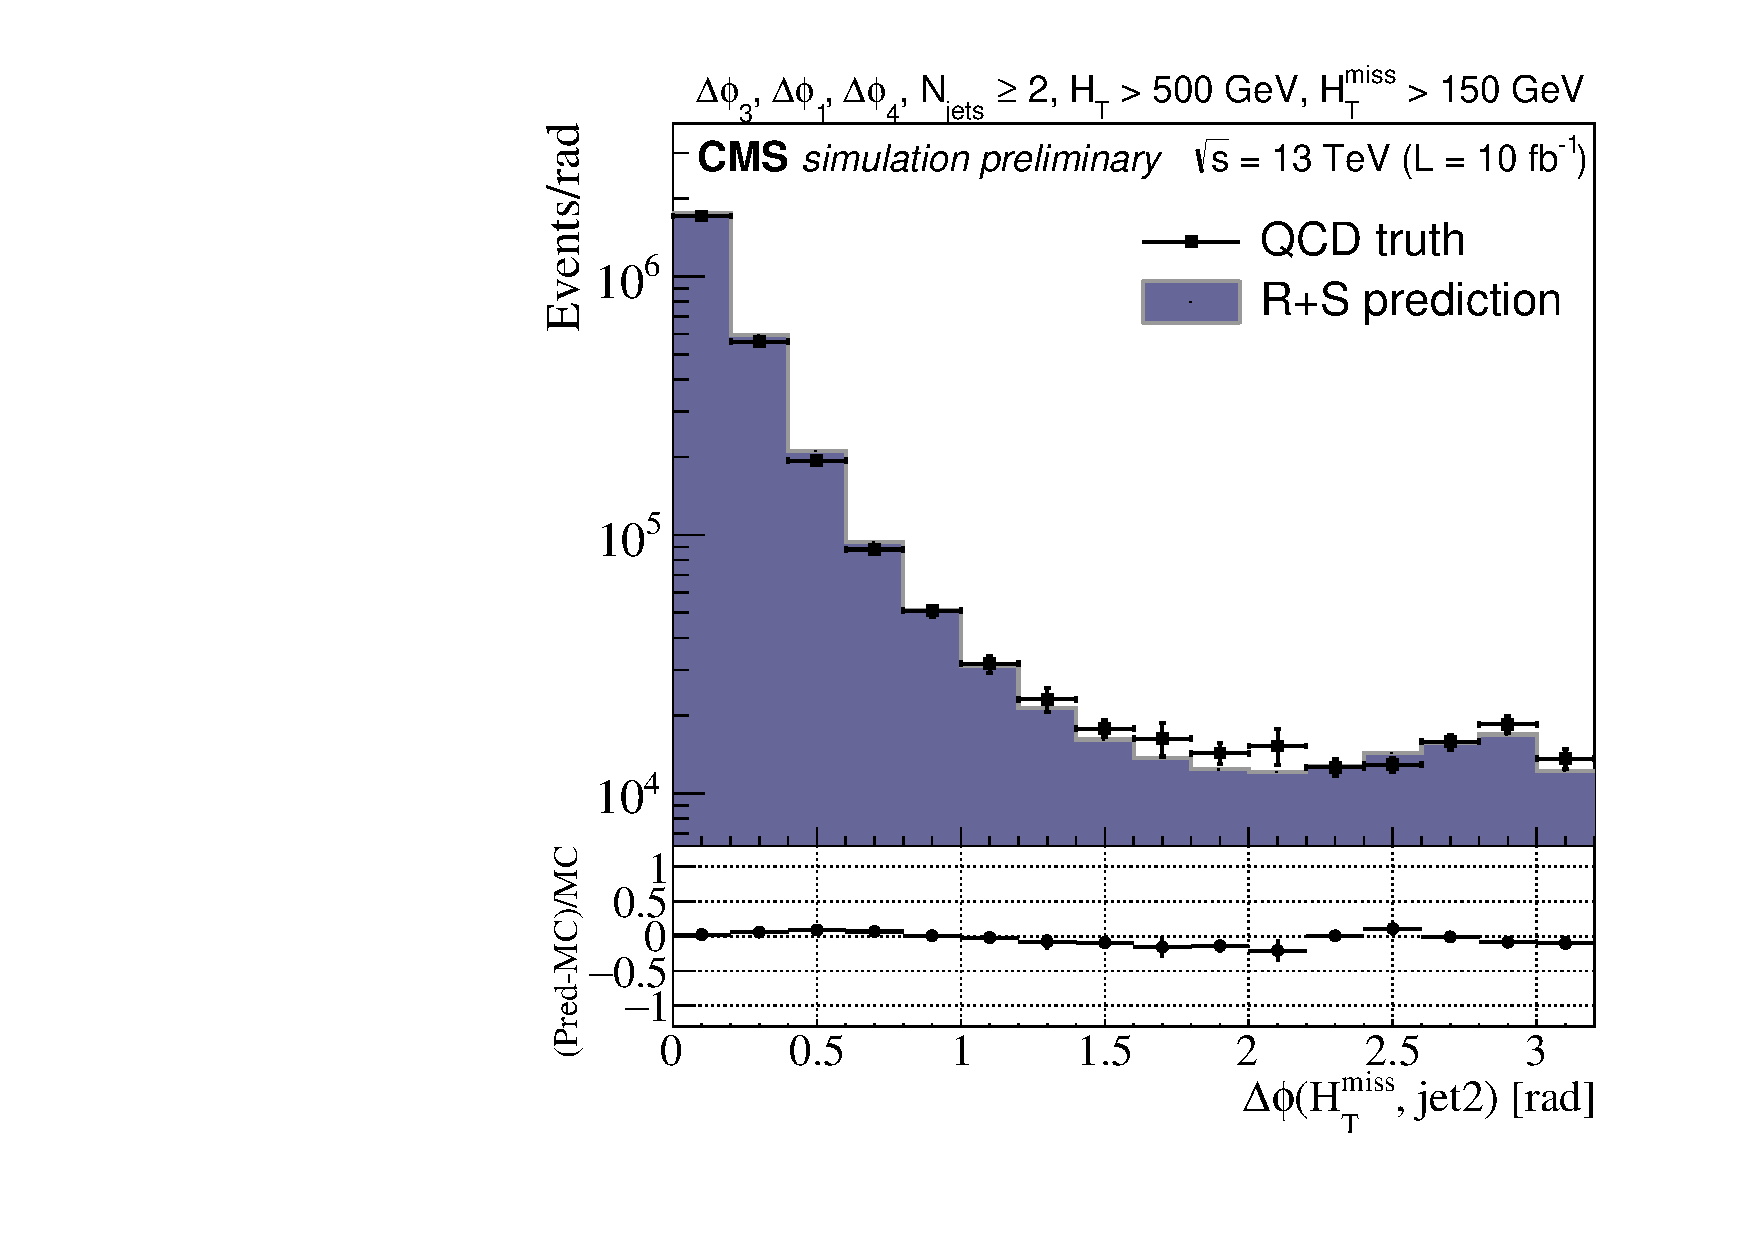
\includegraphics[width=0.5\linewidth]{figures/SusySearches/Ra2b2016/Baseline_DPhi2.pdf}
}\\
\subfloat[]{
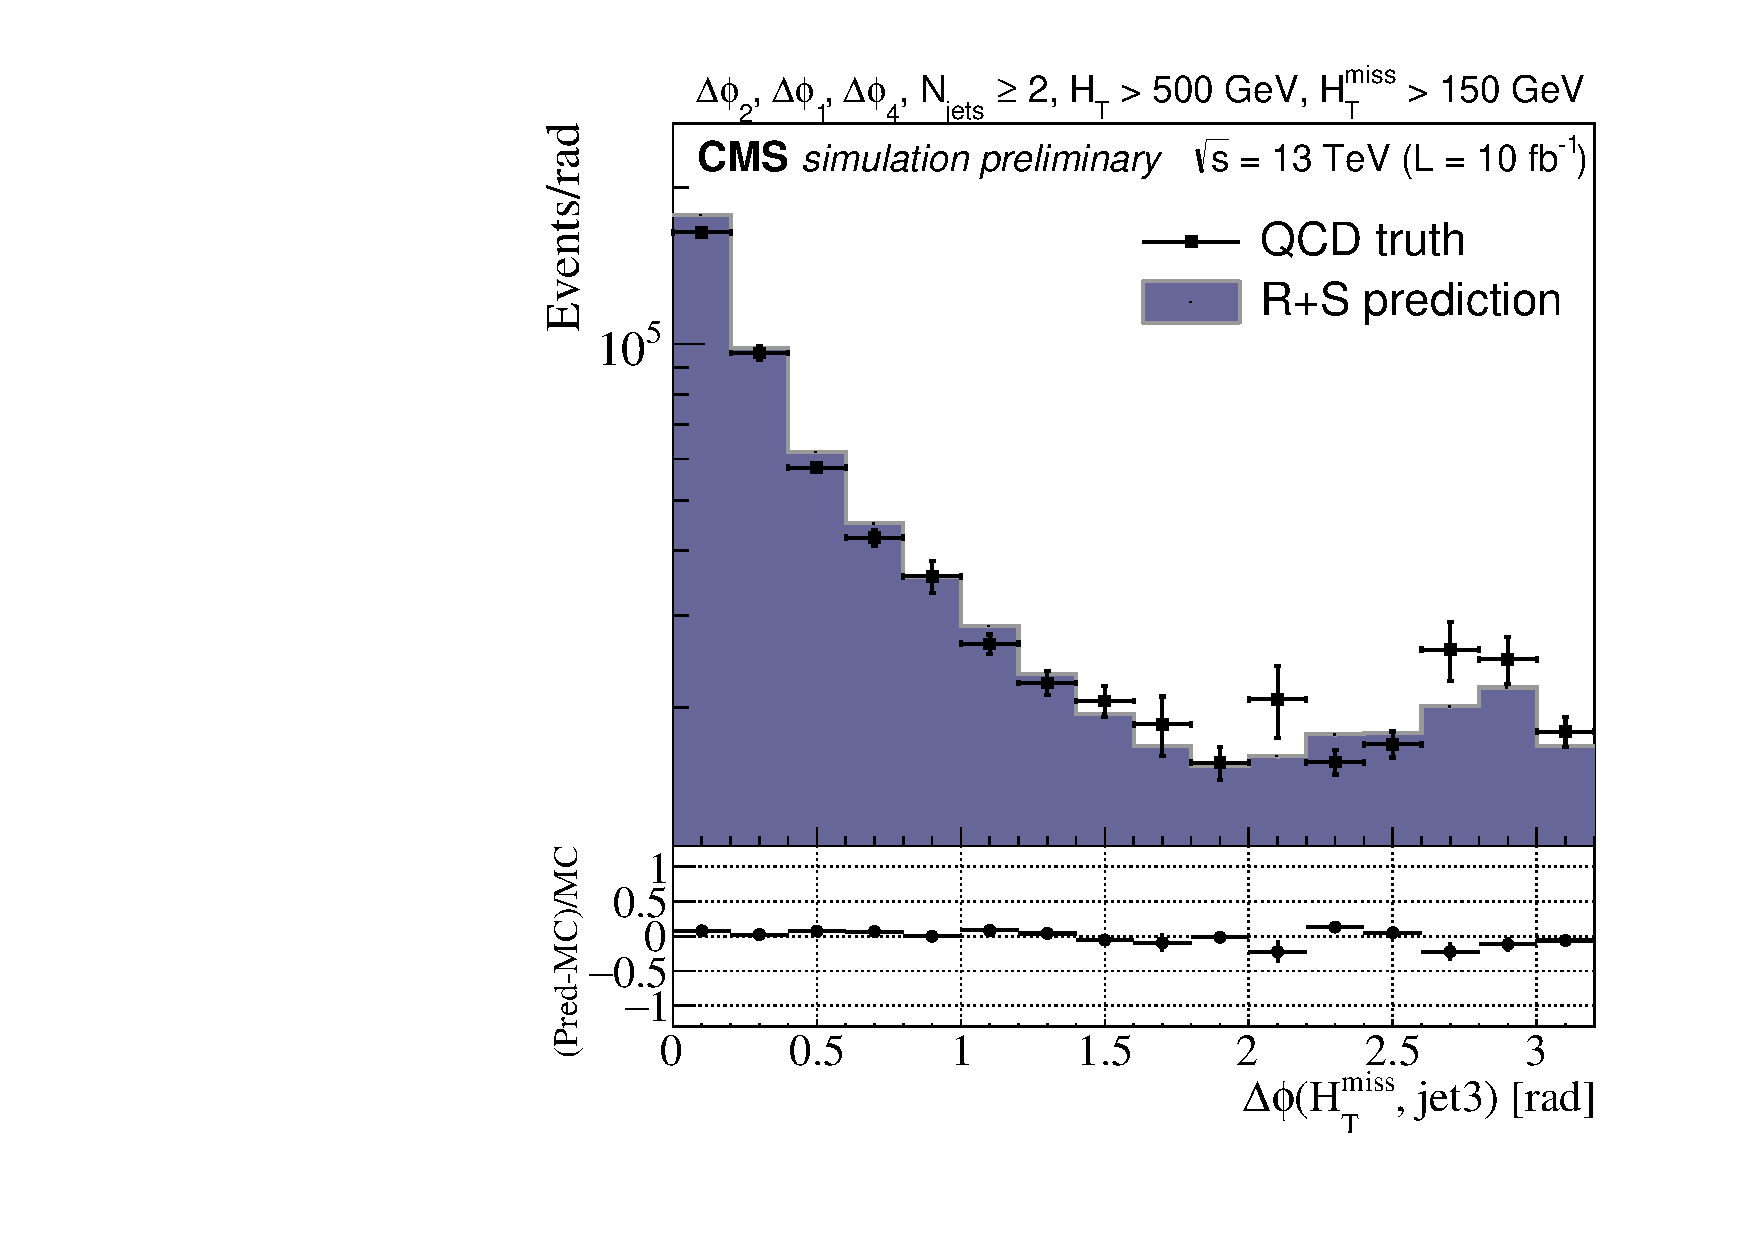
\includegraphics[width=0.5\linewidth]{figures/SusySearches/Ra2b2016/Baseline_DPhi3.pdf}
}
\subfloat[]{
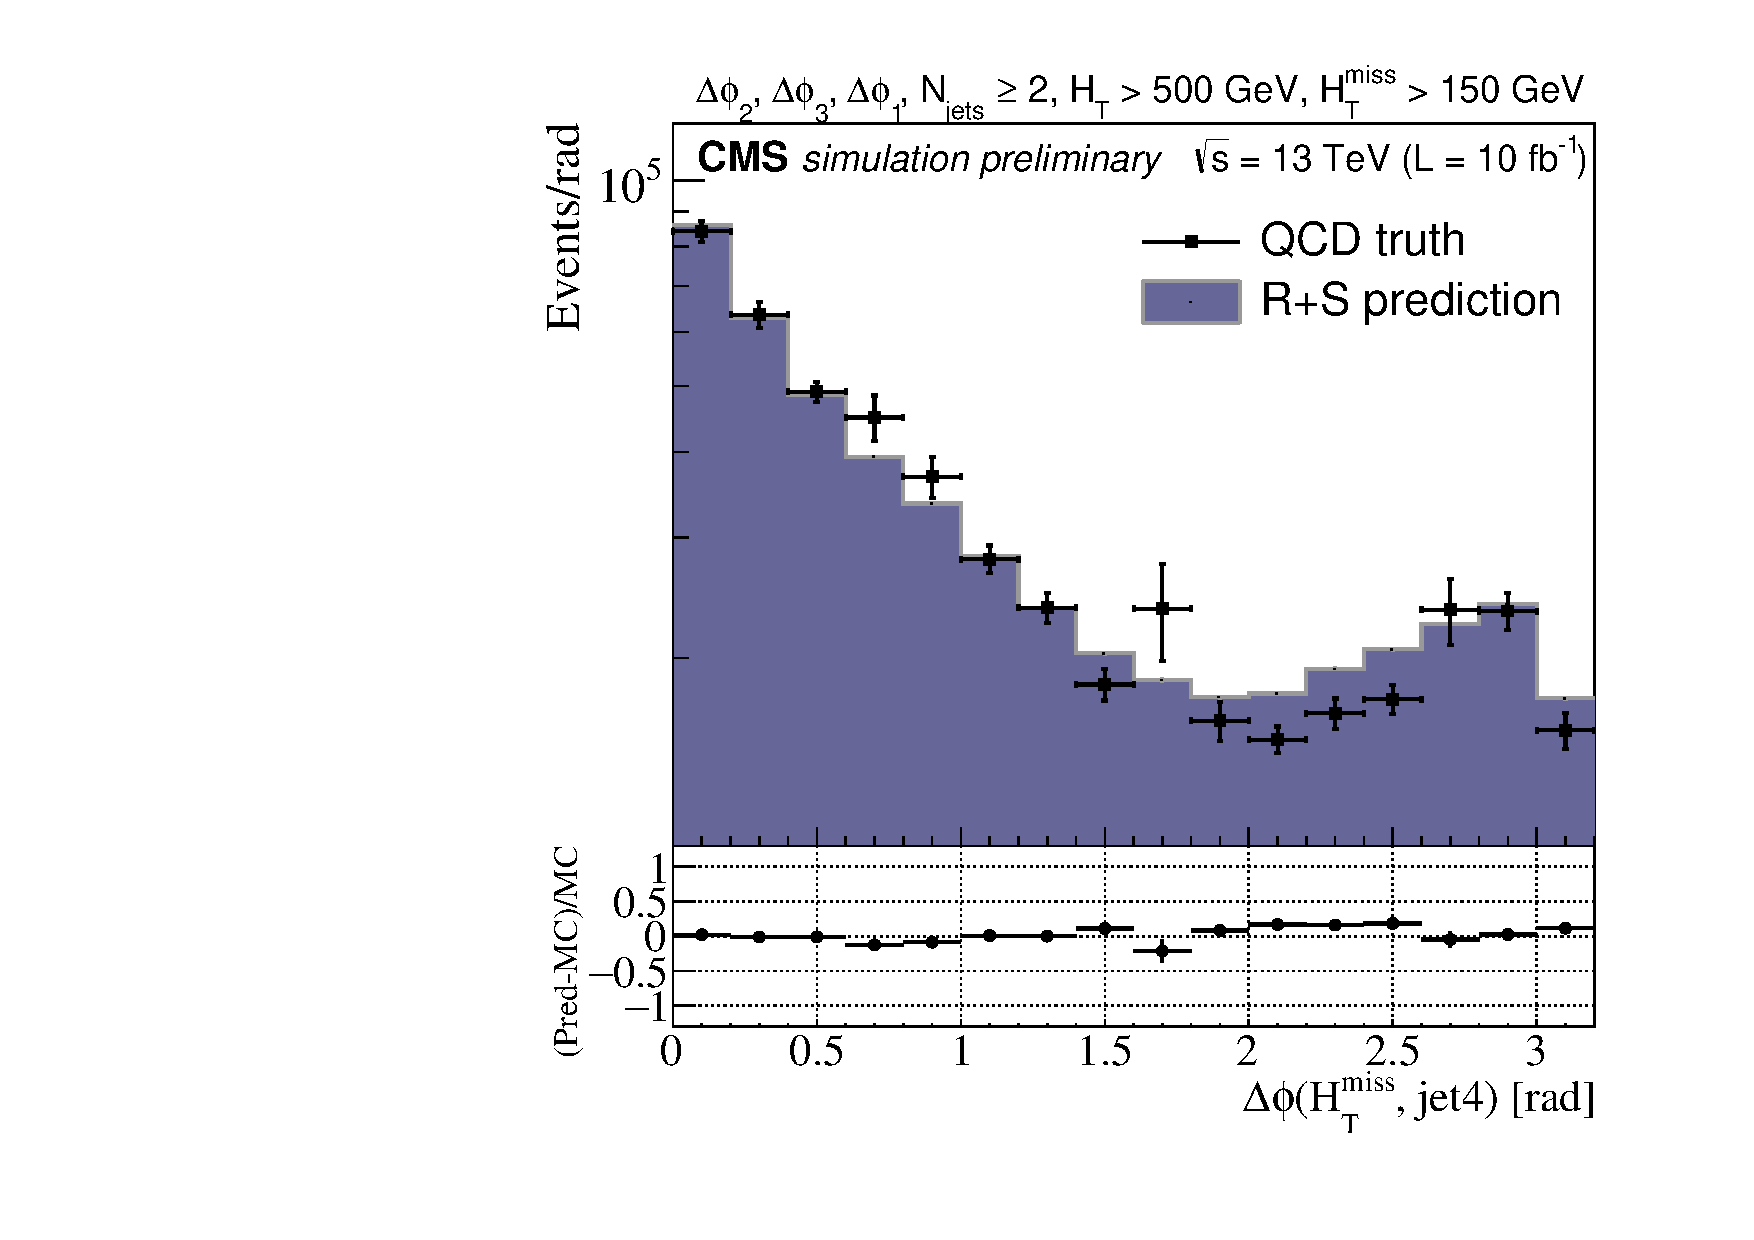
\includegraphics[width=0.5\linewidth]{figures/SusySearches/Ra2b2016/Baseline_DPhi4.pdf}
}
\caption{Comparisons of kinematic distributions between the direct simulation and the rebalance and smear method applied to simulation, after the baseline selection of the multi-jet SUSY search.}
\label{fig:BaselineRplusS2}
\end{figure}

\begin{figure}[h]
\centering
\subfloat[]{
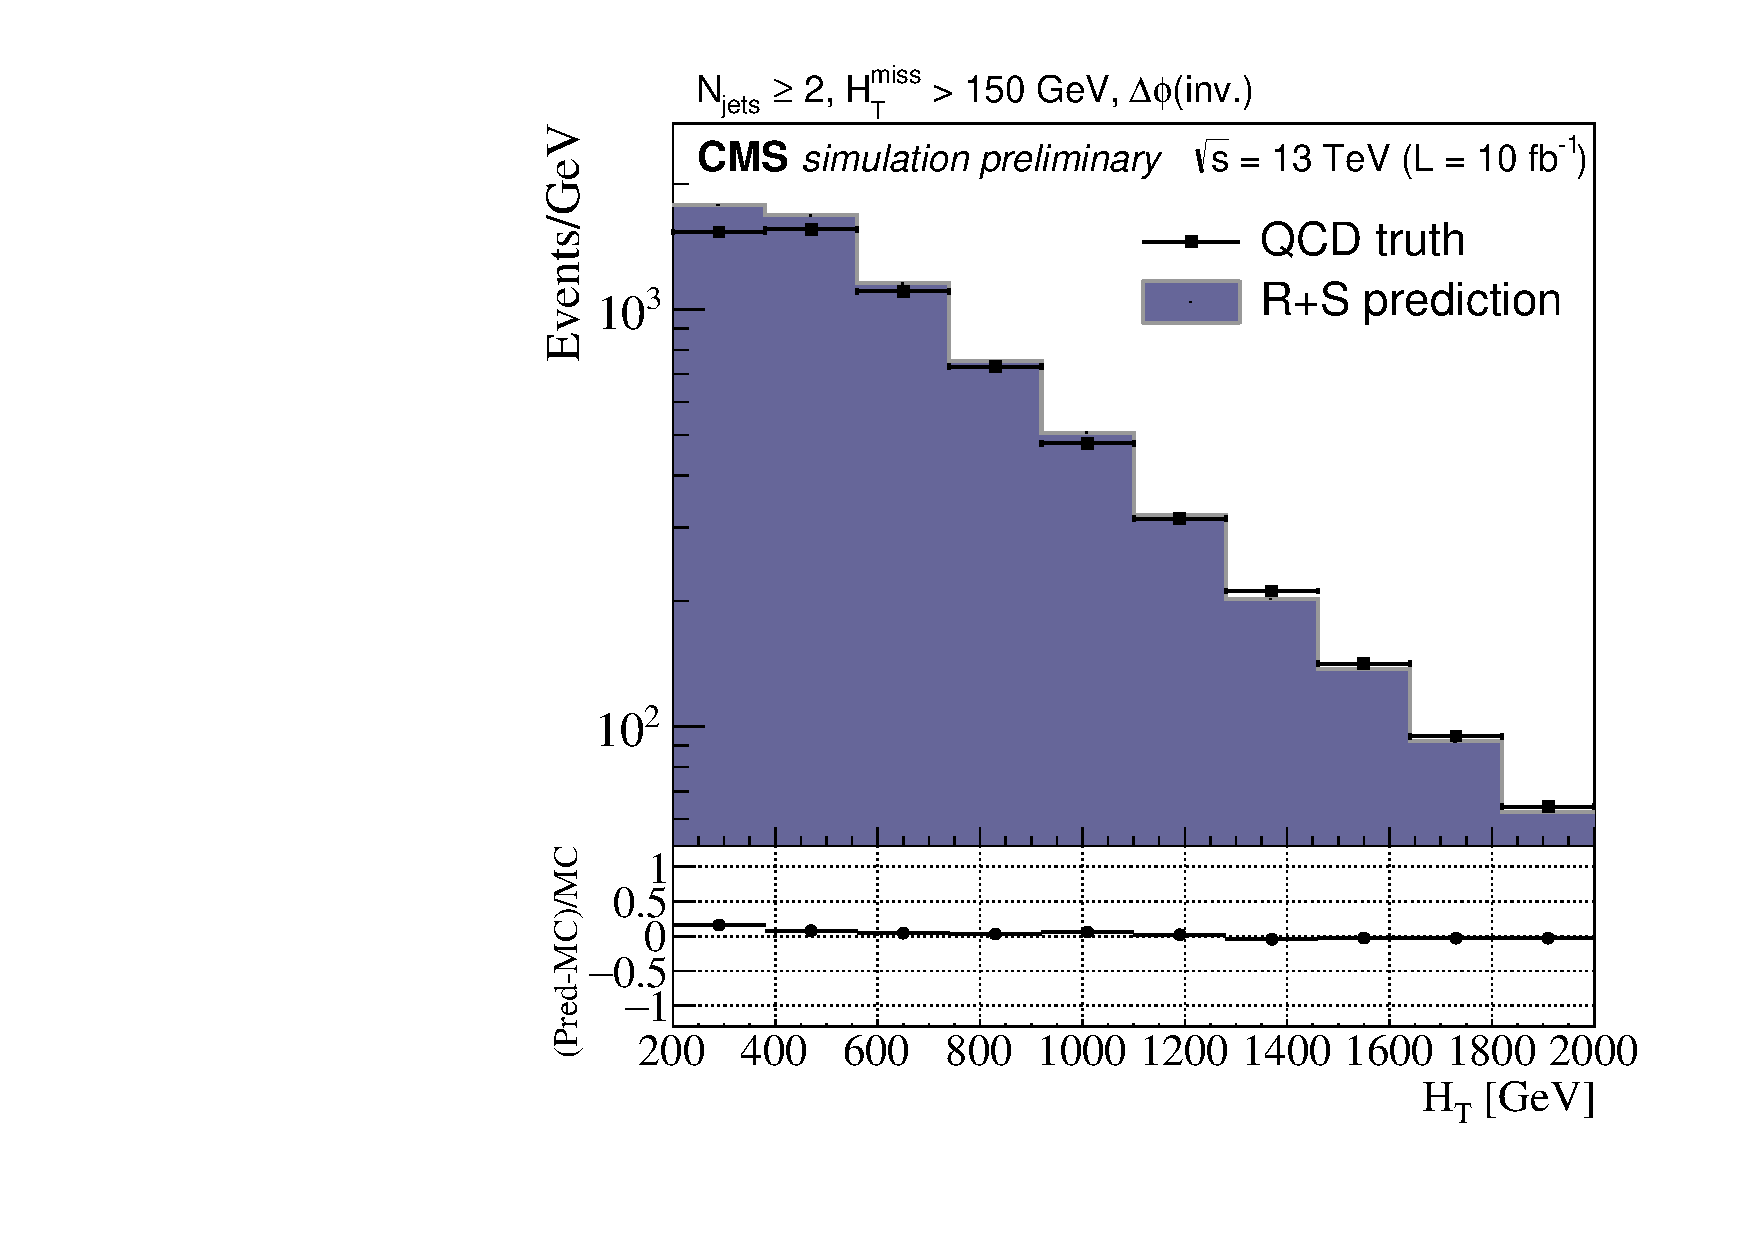
\includegraphics[width=0.5\linewidth]{figures/SusySearches/Ra2b2016/LowDeltaPhi_Ht.pdf}
}
\subfloat[]{
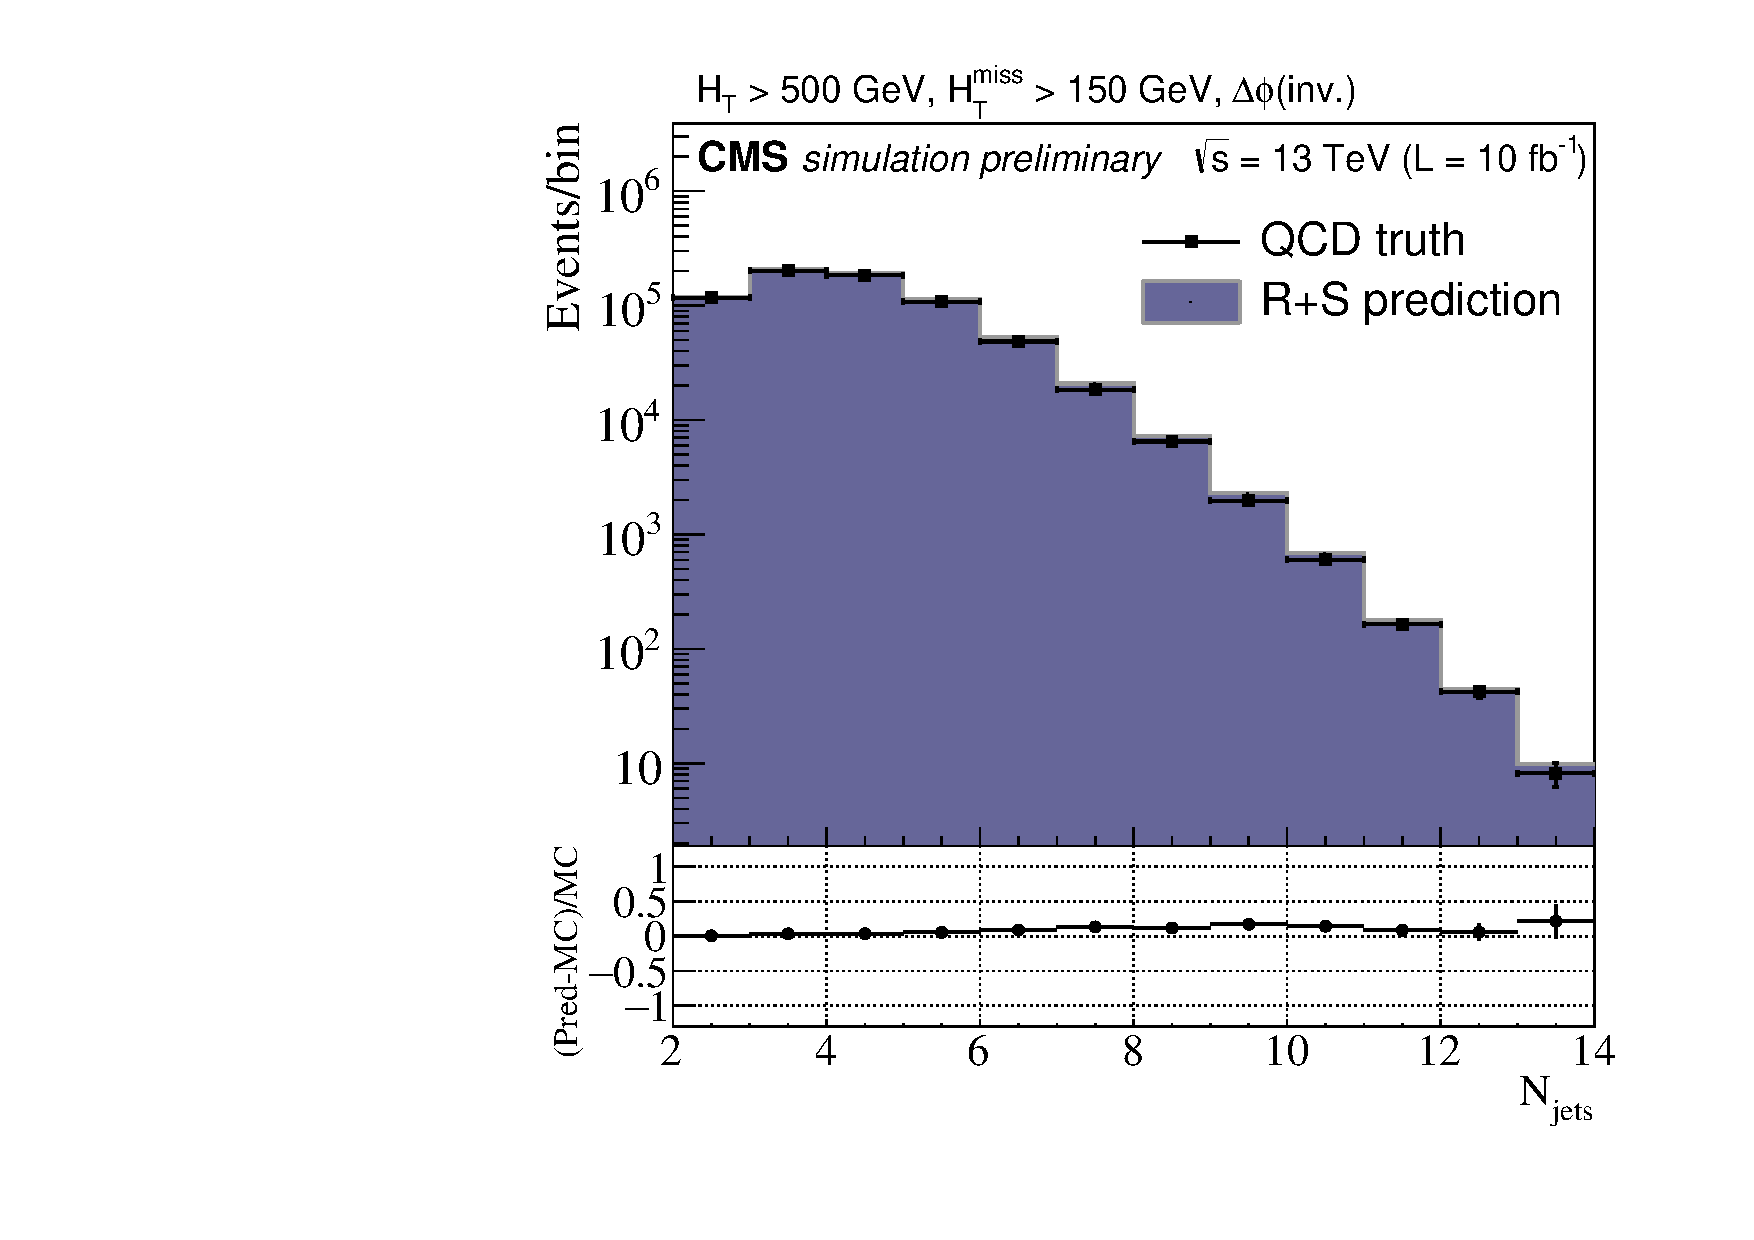
\includegraphics[width=0.5\linewidth]{figures/SusySearches/Ra2b2016/LowDeltaPhi_NJets.pdf}
}\\
\subfloat[]{
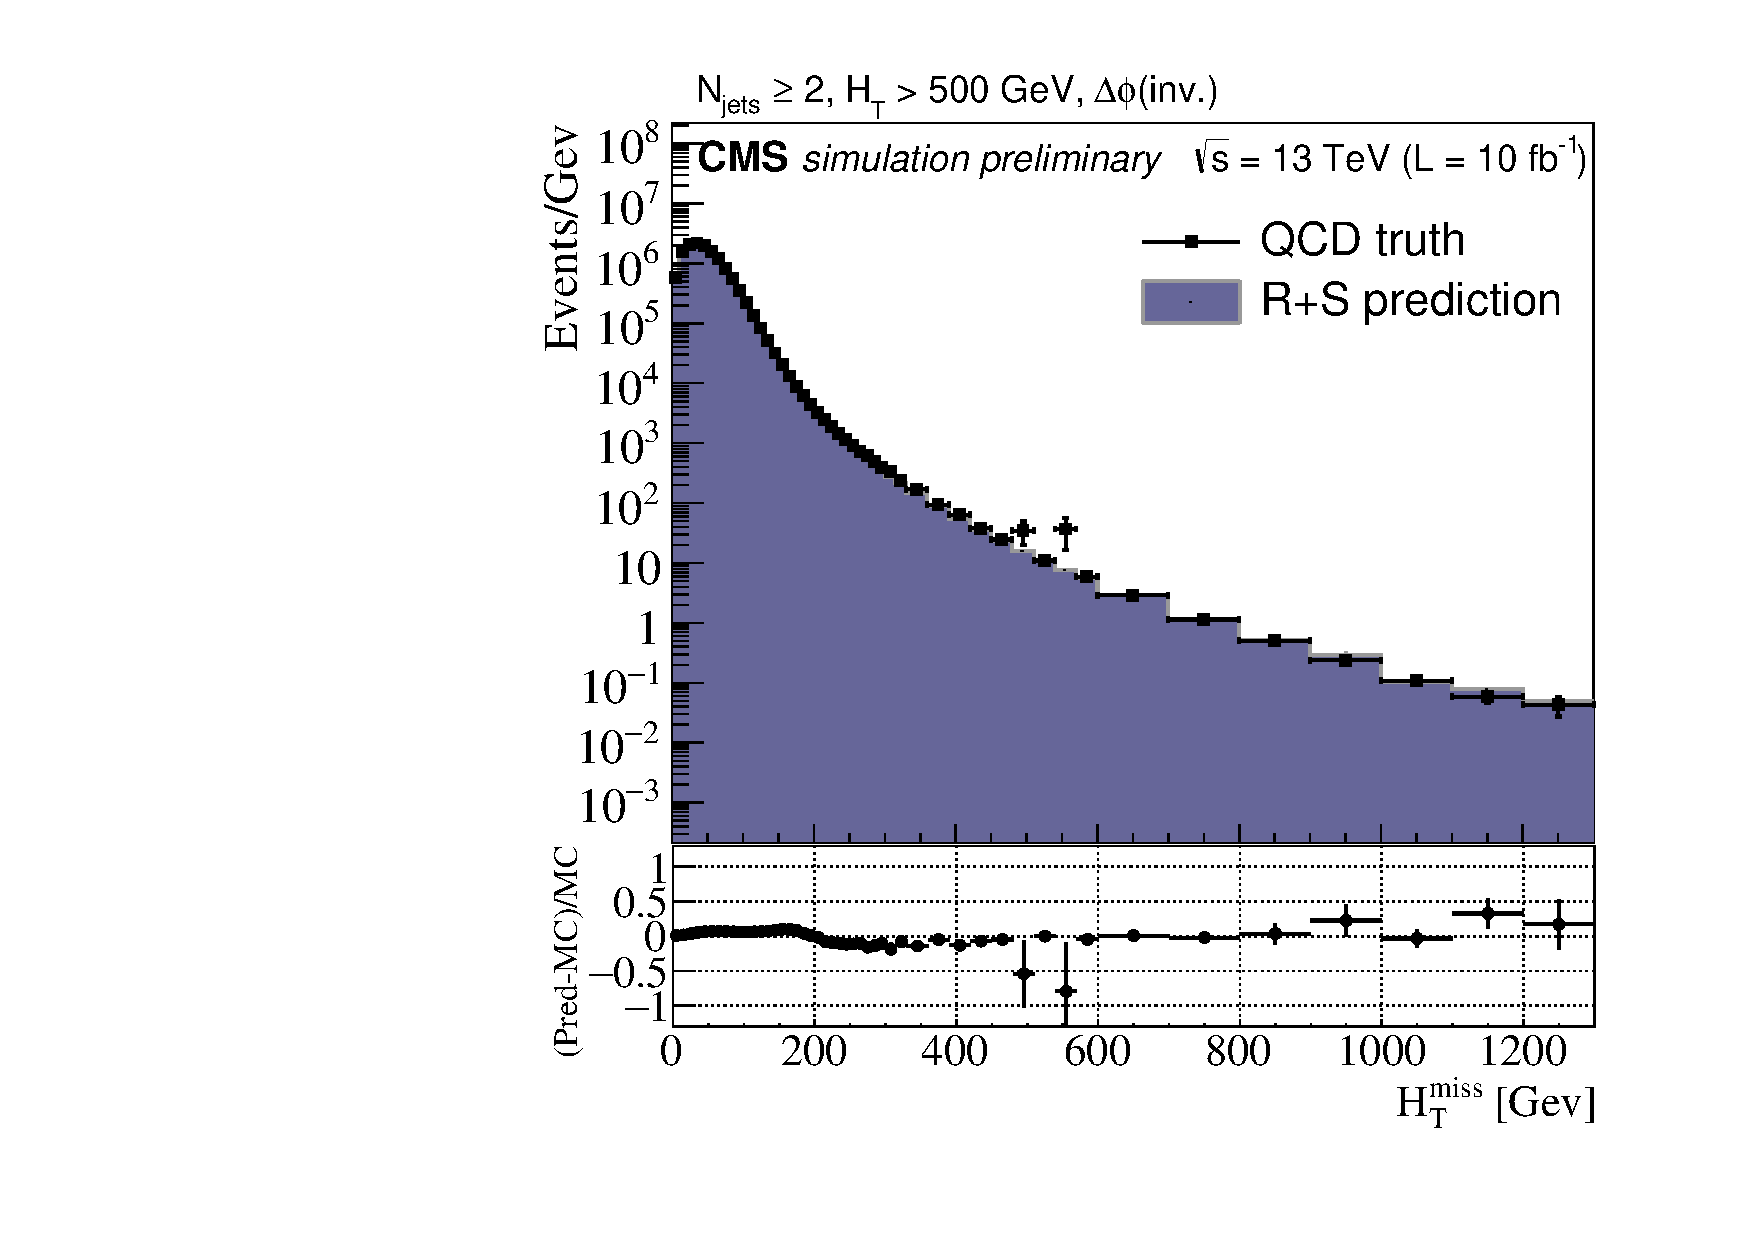
\includegraphics[width=0.5\linewidth]{figures/SusySearches/Ra2b2016/LowDeltaPhi_Mht.pdf}
}
\subfloat[]{
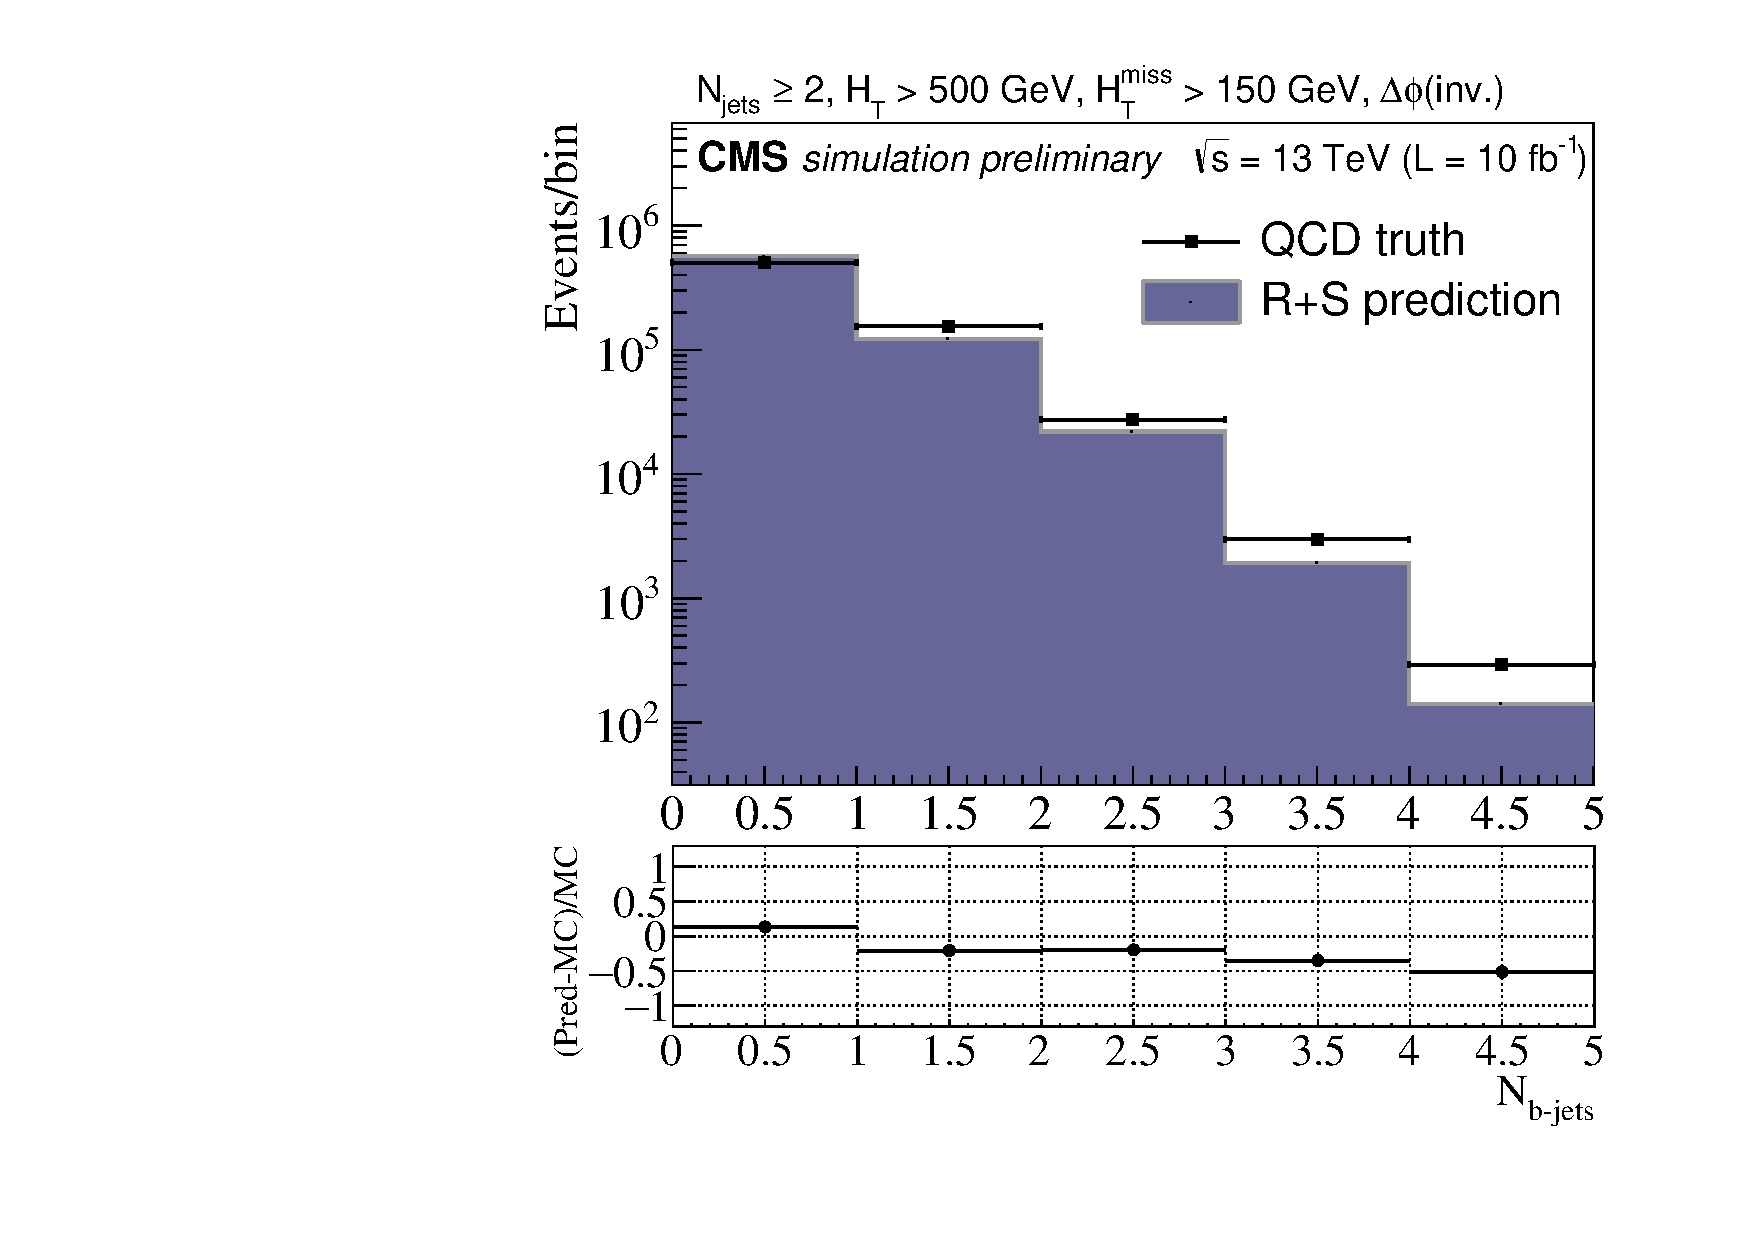
\includegraphics[width=0.5\linewidth]{figures/SusySearches/Ra2b2016/LowDeltaPhi_BTags.pdf}
}
\caption{Comparisons of kinematic distributions between the direct simulation and the rebalance and smear method applied to simulation, in the inverted $\Delta \phi$ control region of the multi-jet SUSY search.}
\label{fig:LowDeltaPhiRplusS}
\end{figure}


\begin{figure}[h]
\centering
\subfloat[]{
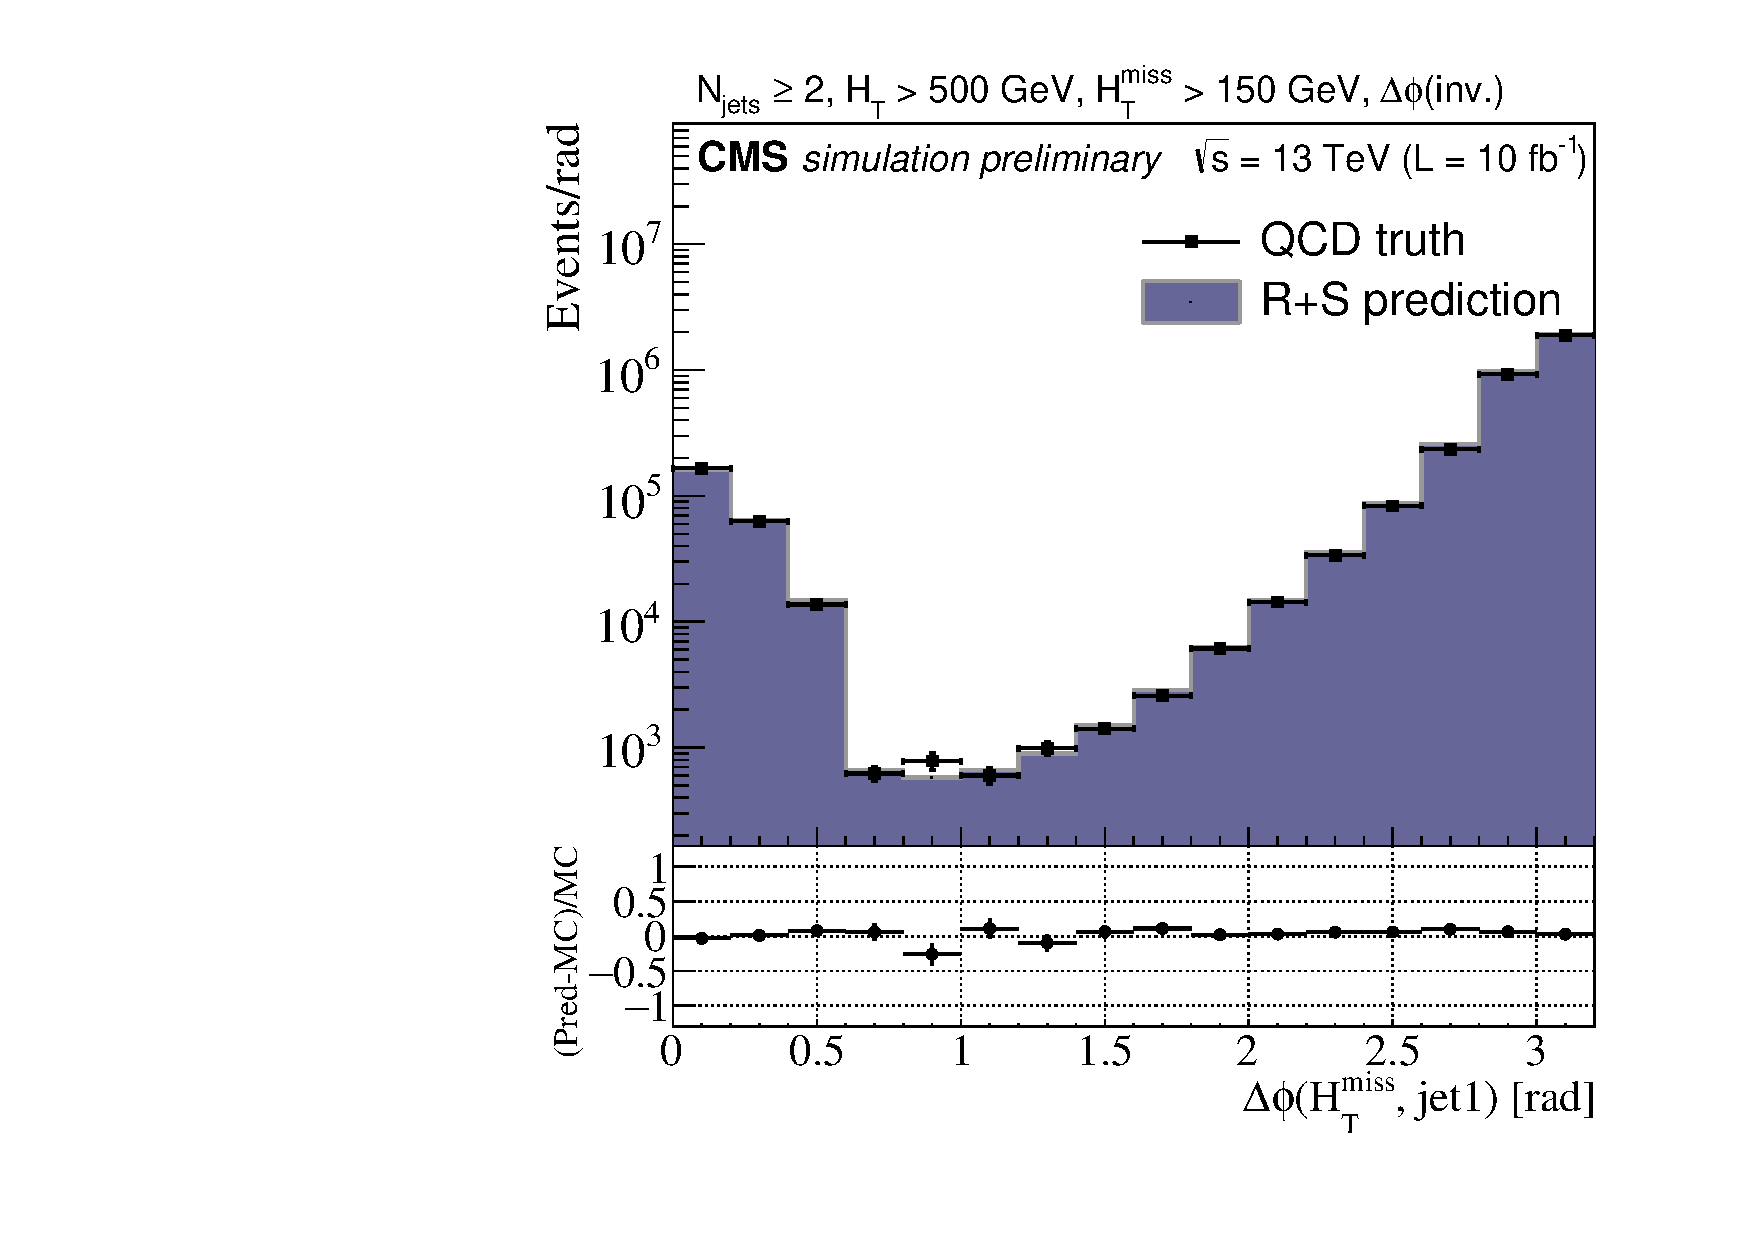
\includegraphics[width=0.5\linewidth]{figures/SusySearches/Ra2b2016/LowDeltaPhi_DPhi1.pdf}
}
\subfloat[]{
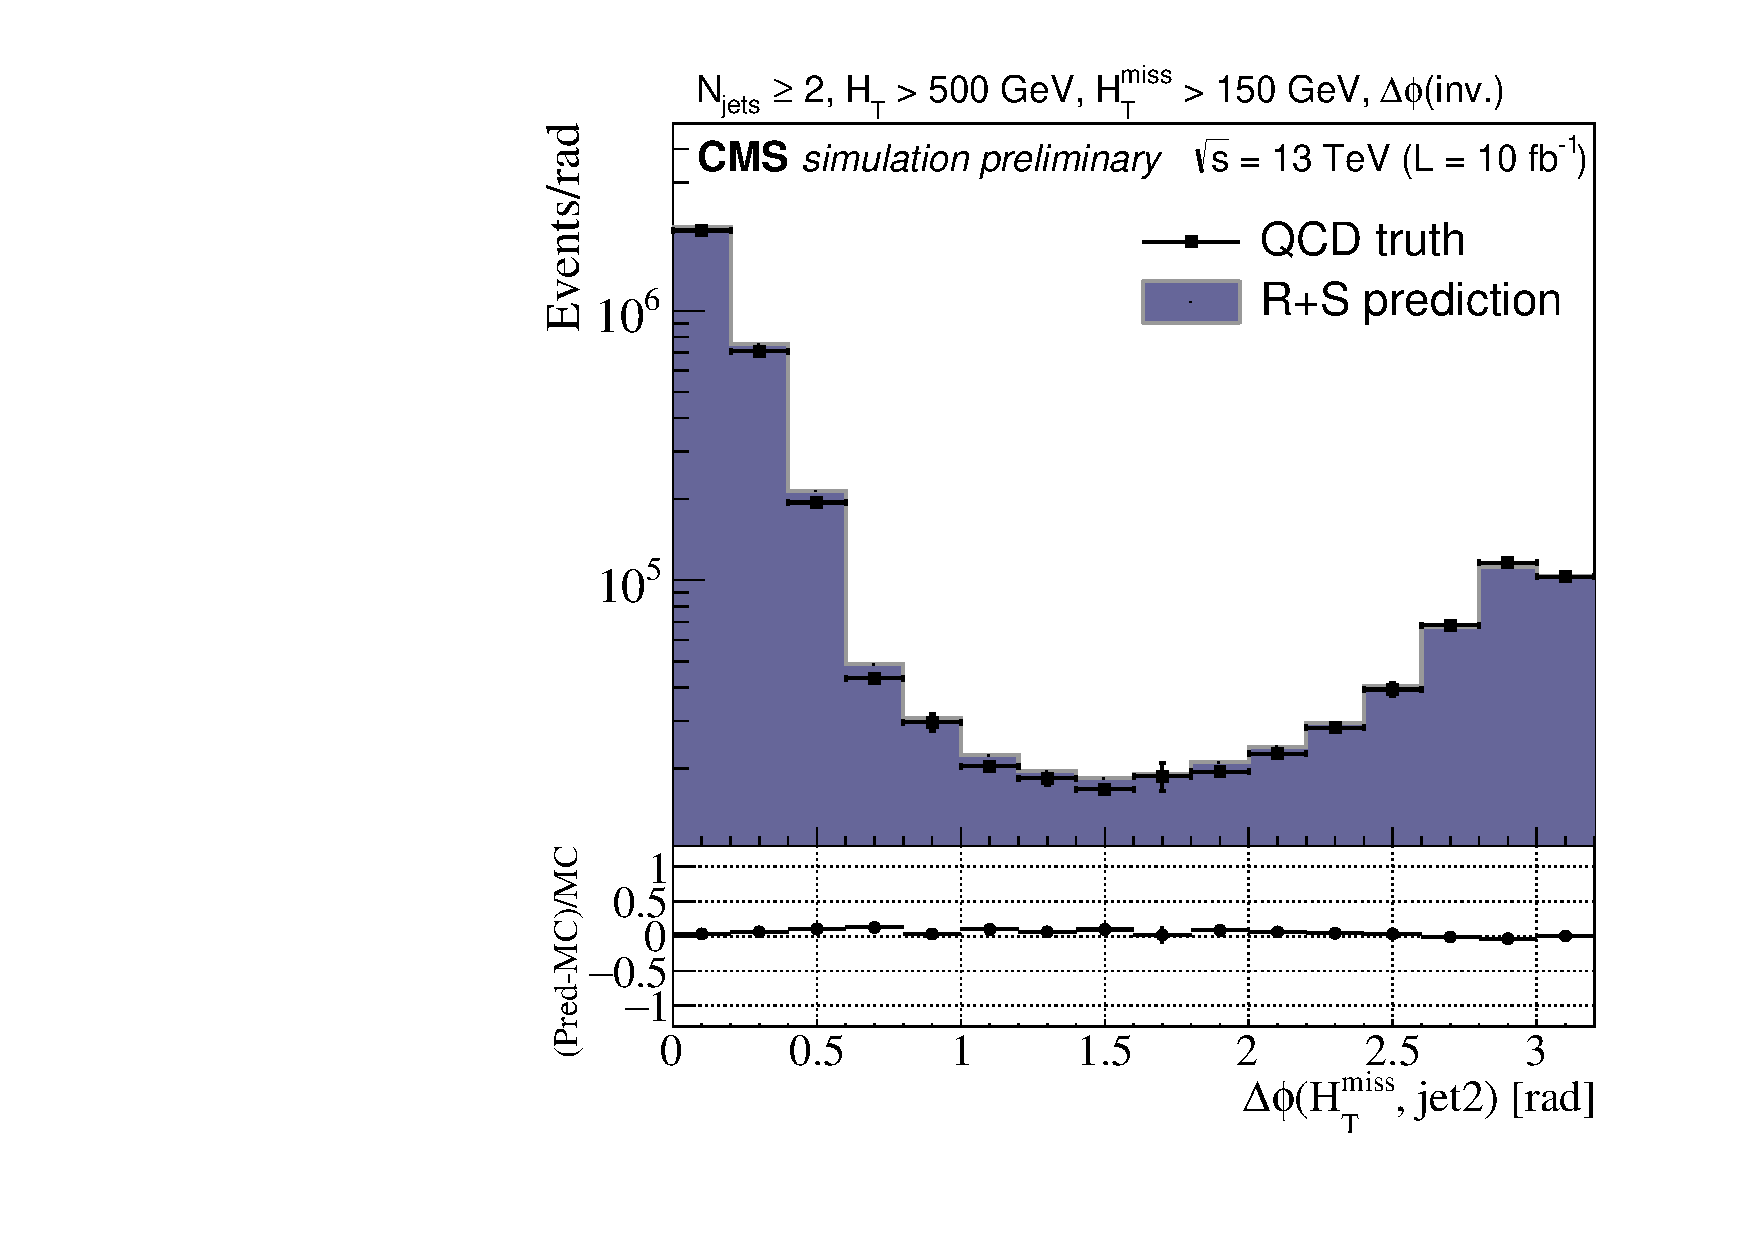
\includegraphics[width=0.5\linewidth]{figures/SusySearches/Ra2b2016/LowDeltaPhi_DPhi2.pdf}
}\\
\subfloat[]{
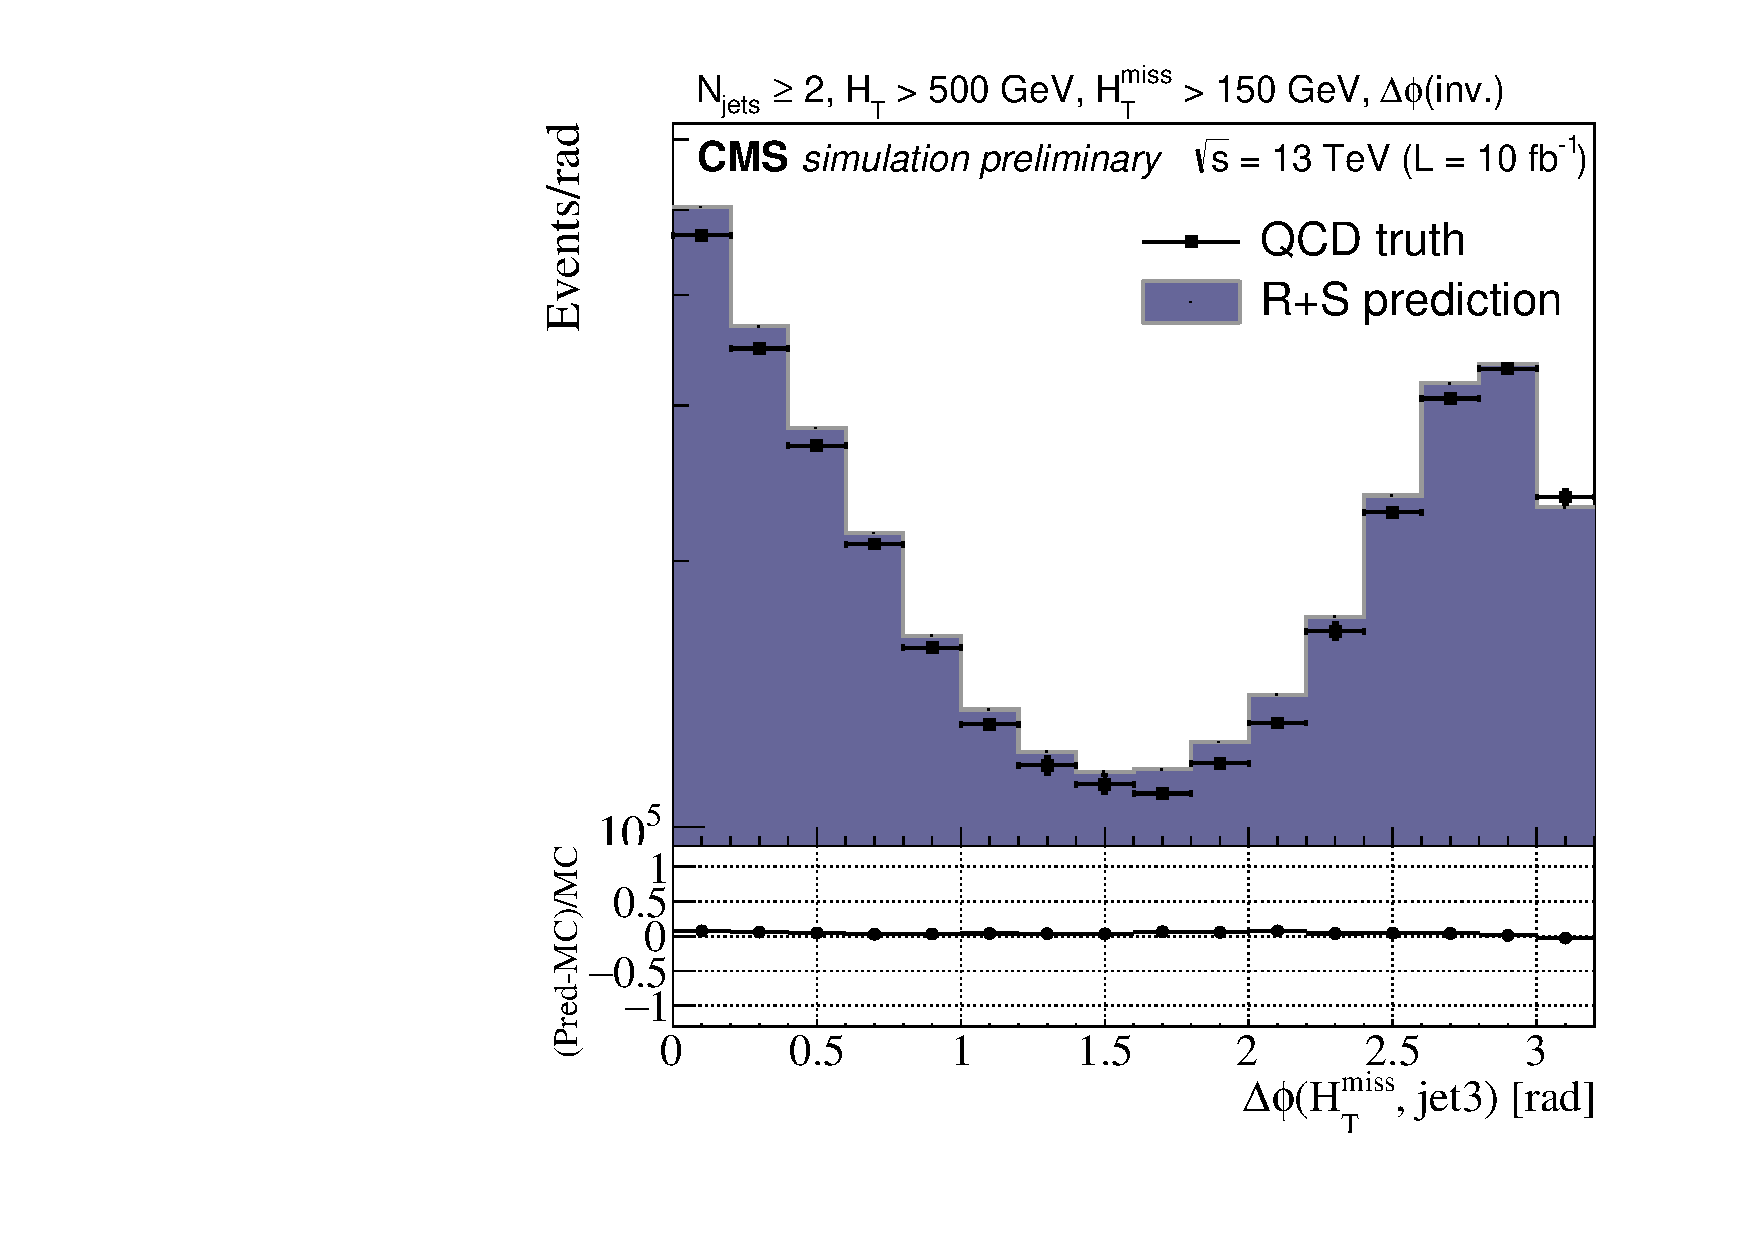
\includegraphics[width=0.5\linewidth]{figures/SusySearches/Ra2b2016/LowDeltaPhi_DPhi3.pdf}
}
\subfloat[]{
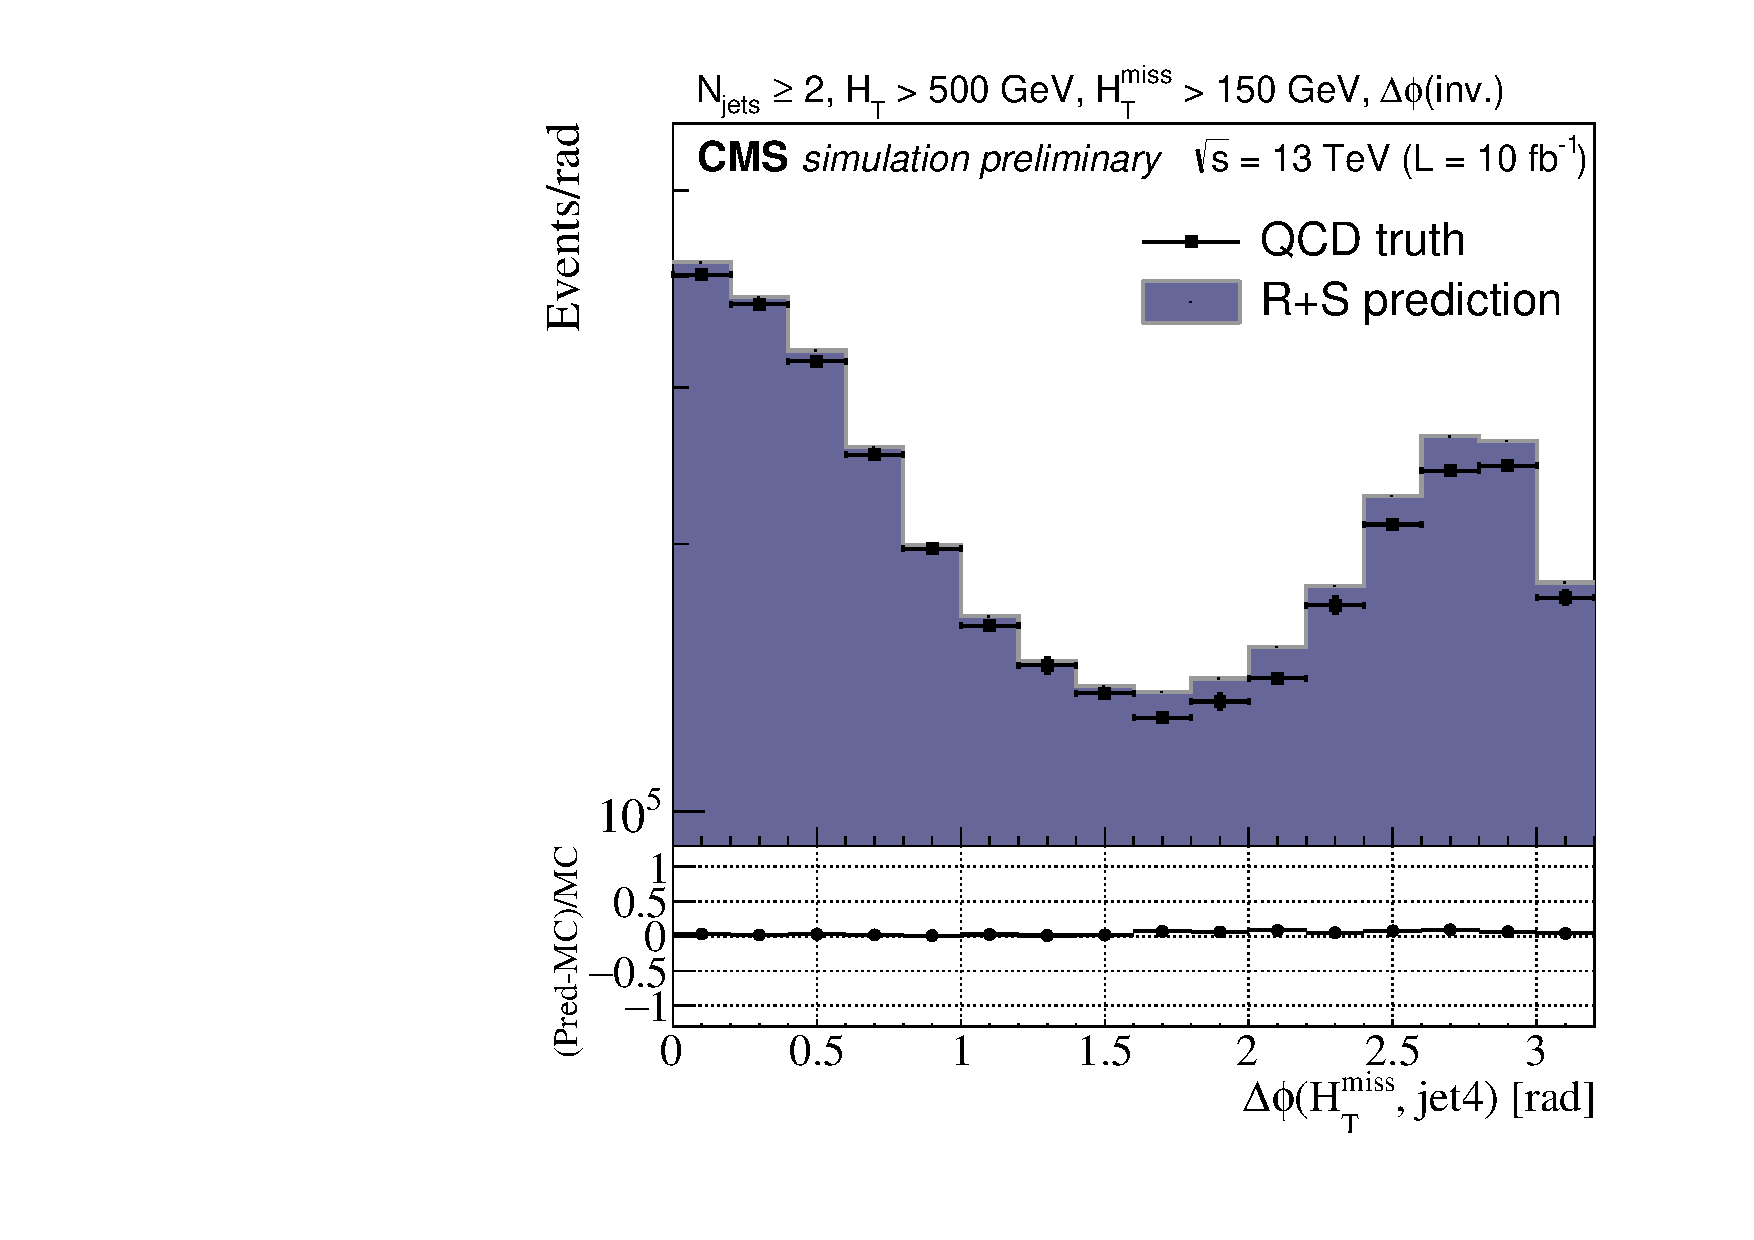
\includegraphics[width=0.5\linewidth]{figures/SusySearches/Ra2b2016/LowDeltaPhi_DPhi4.pdf}
}
\caption{Comparisons of kinematic distributions between the direct simulation and the rebalance and smear method applied to simulation, in the inverted $\Delta \phi$ control region of the multi-jet SUSY search.}
\label{fig:LowDeltaPhiRplusS2}
\end{figure}

\begin{figure}[h]
\centering
\subfloat[]{
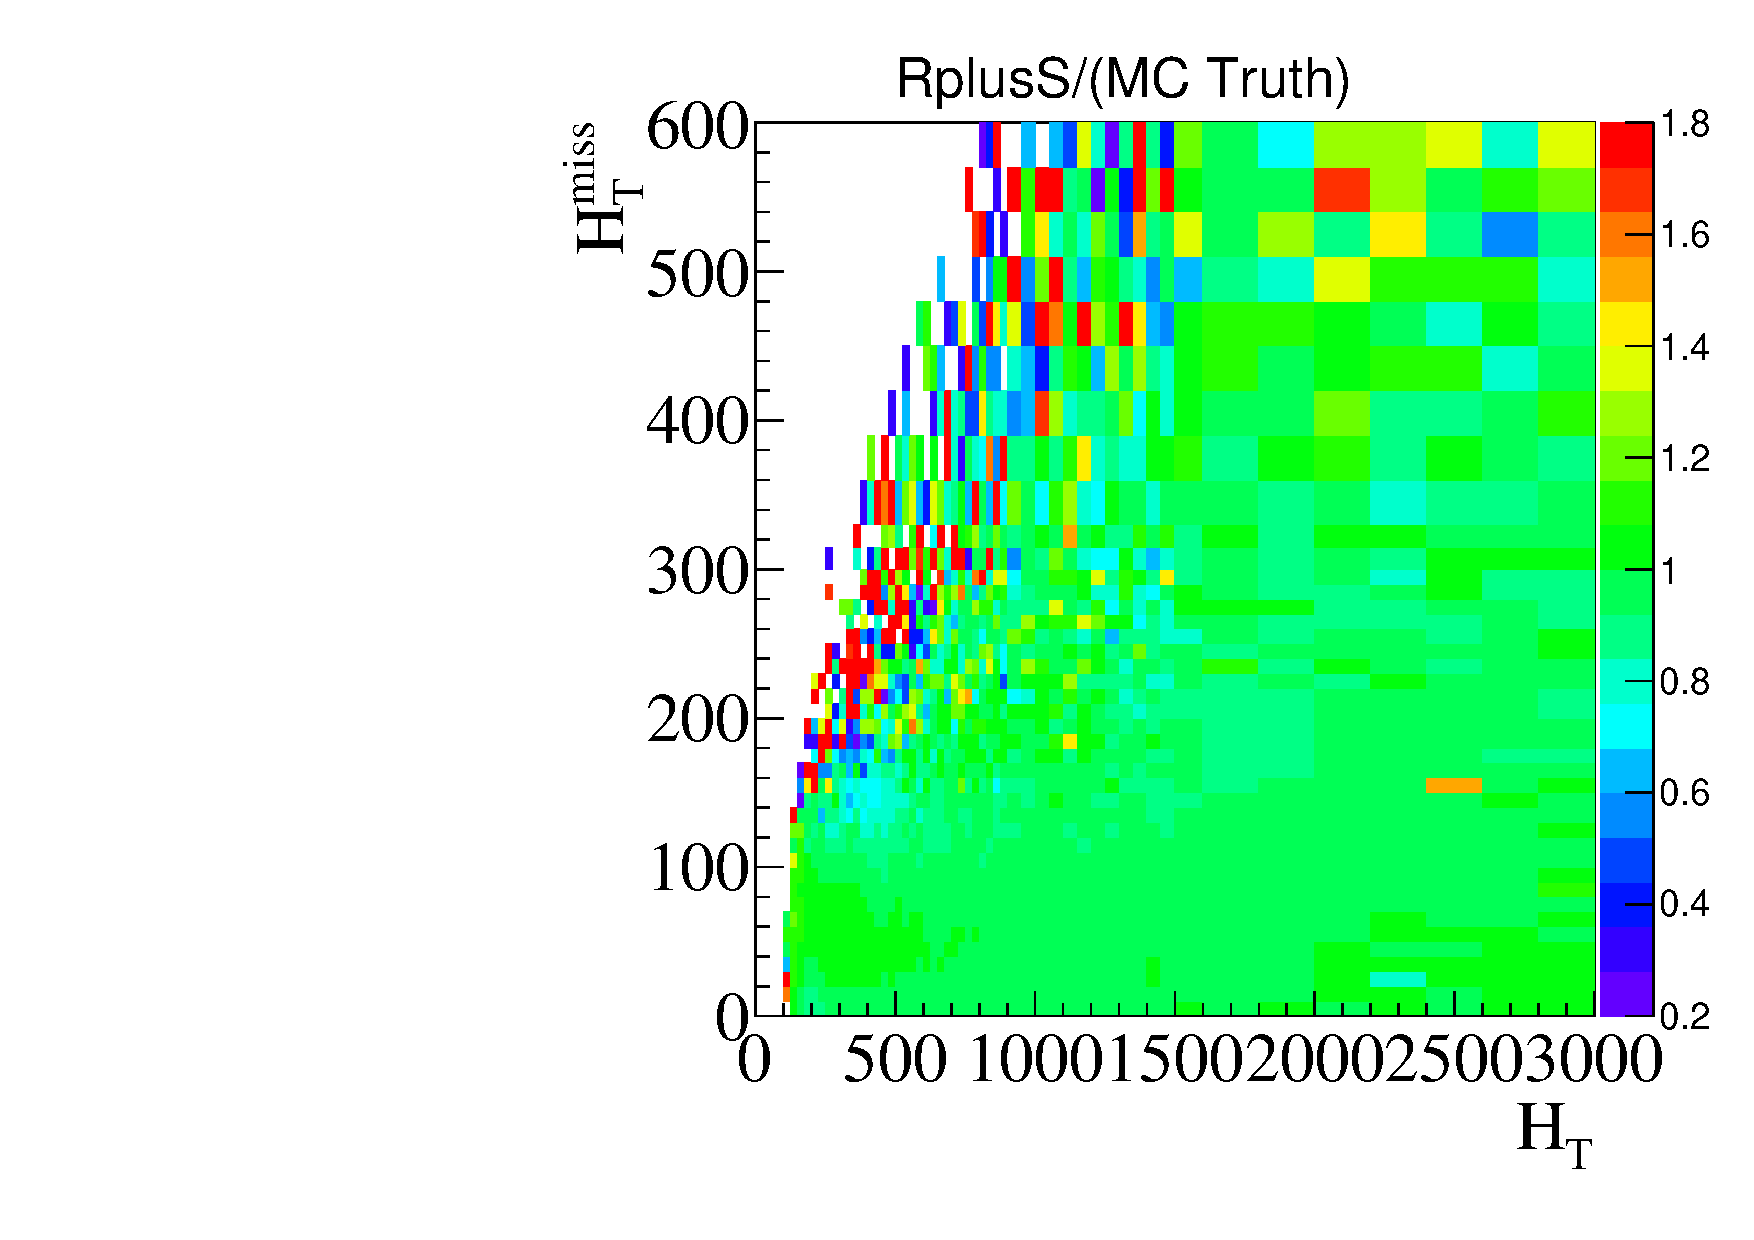
\includegraphics[width=0.5\linewidth]{figures/SusySearches/Ra2b2016/RplusSAndTruth_MhtVsHt.pdf}
}
\subfloat[]{
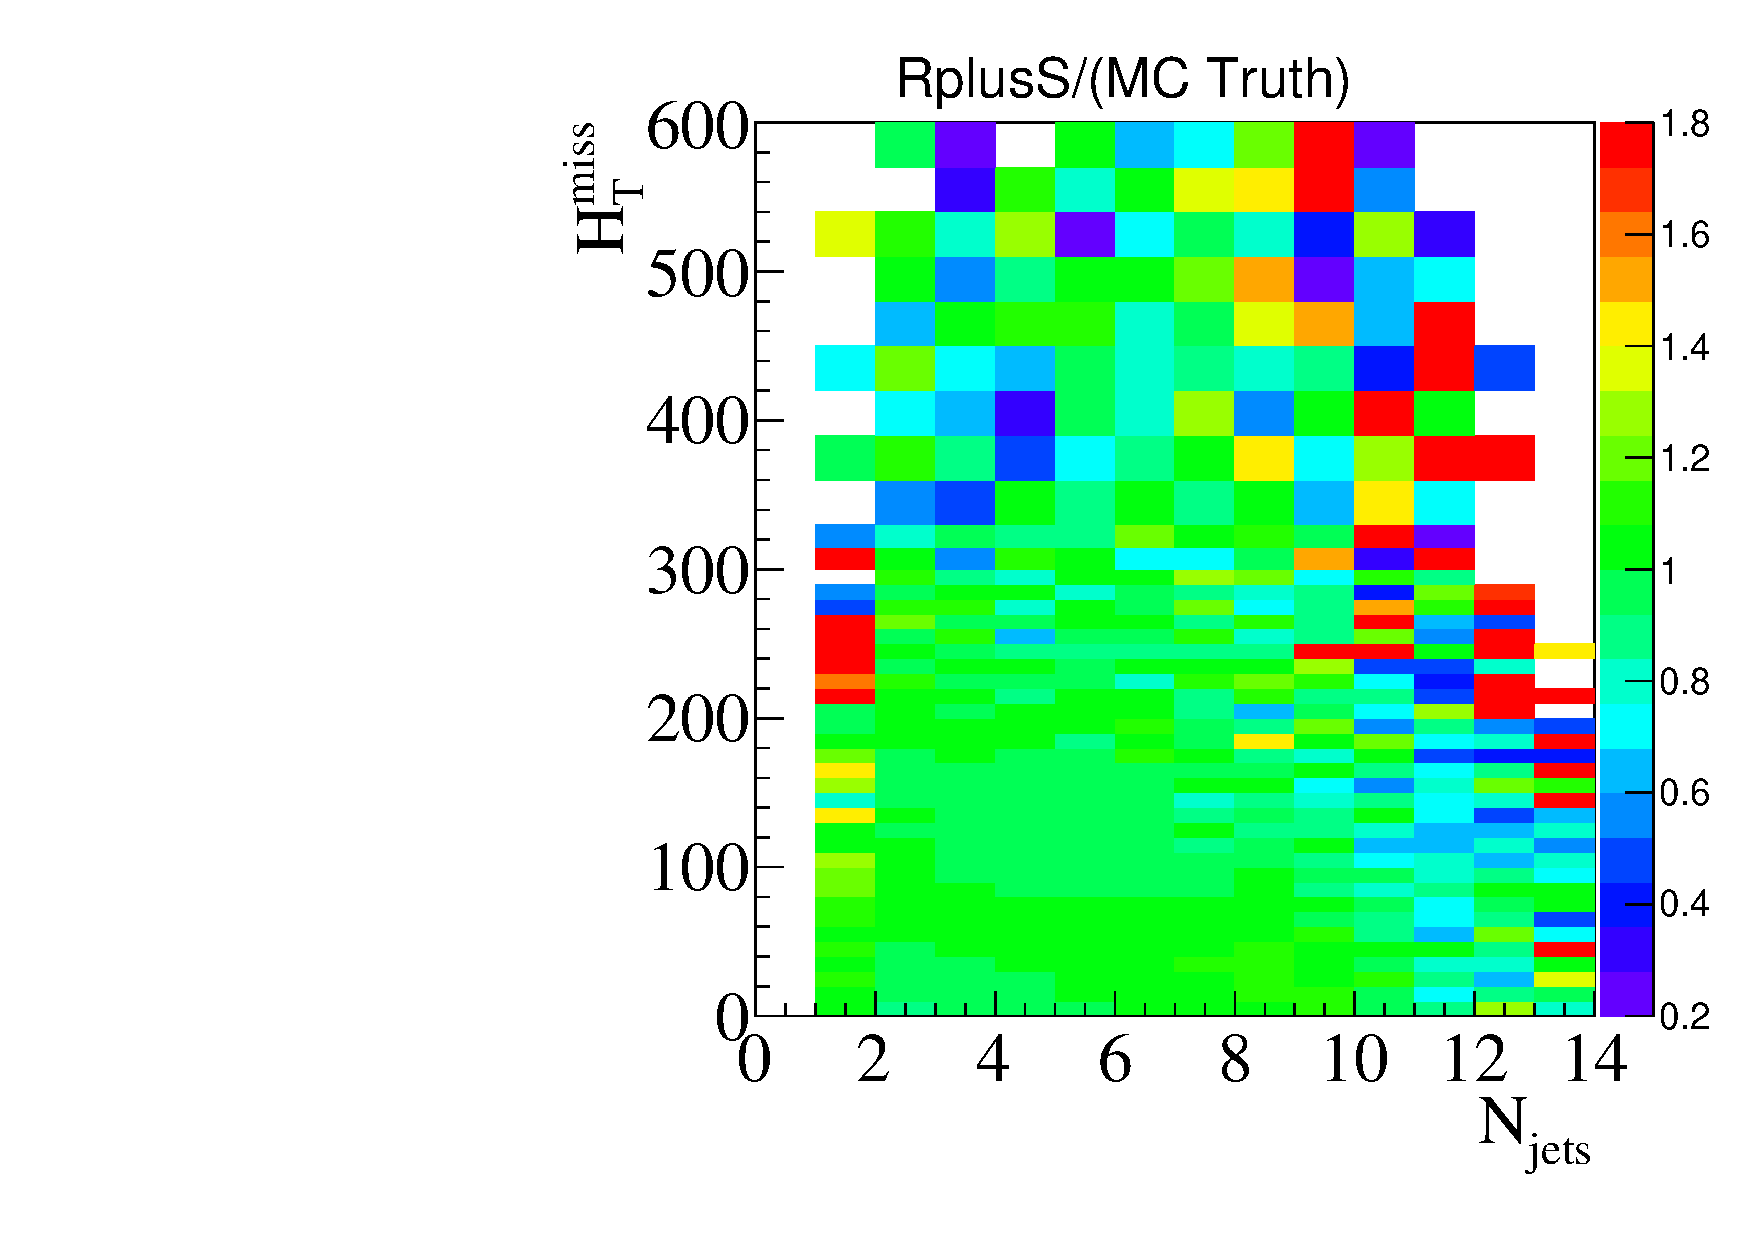
\includegraphics[width=0.5\linewidth]{figures/SusySearches/Ra2b2016/RplusSAndTruth_MhtVsNJets.pdf}
}\\
\subfloat[]{
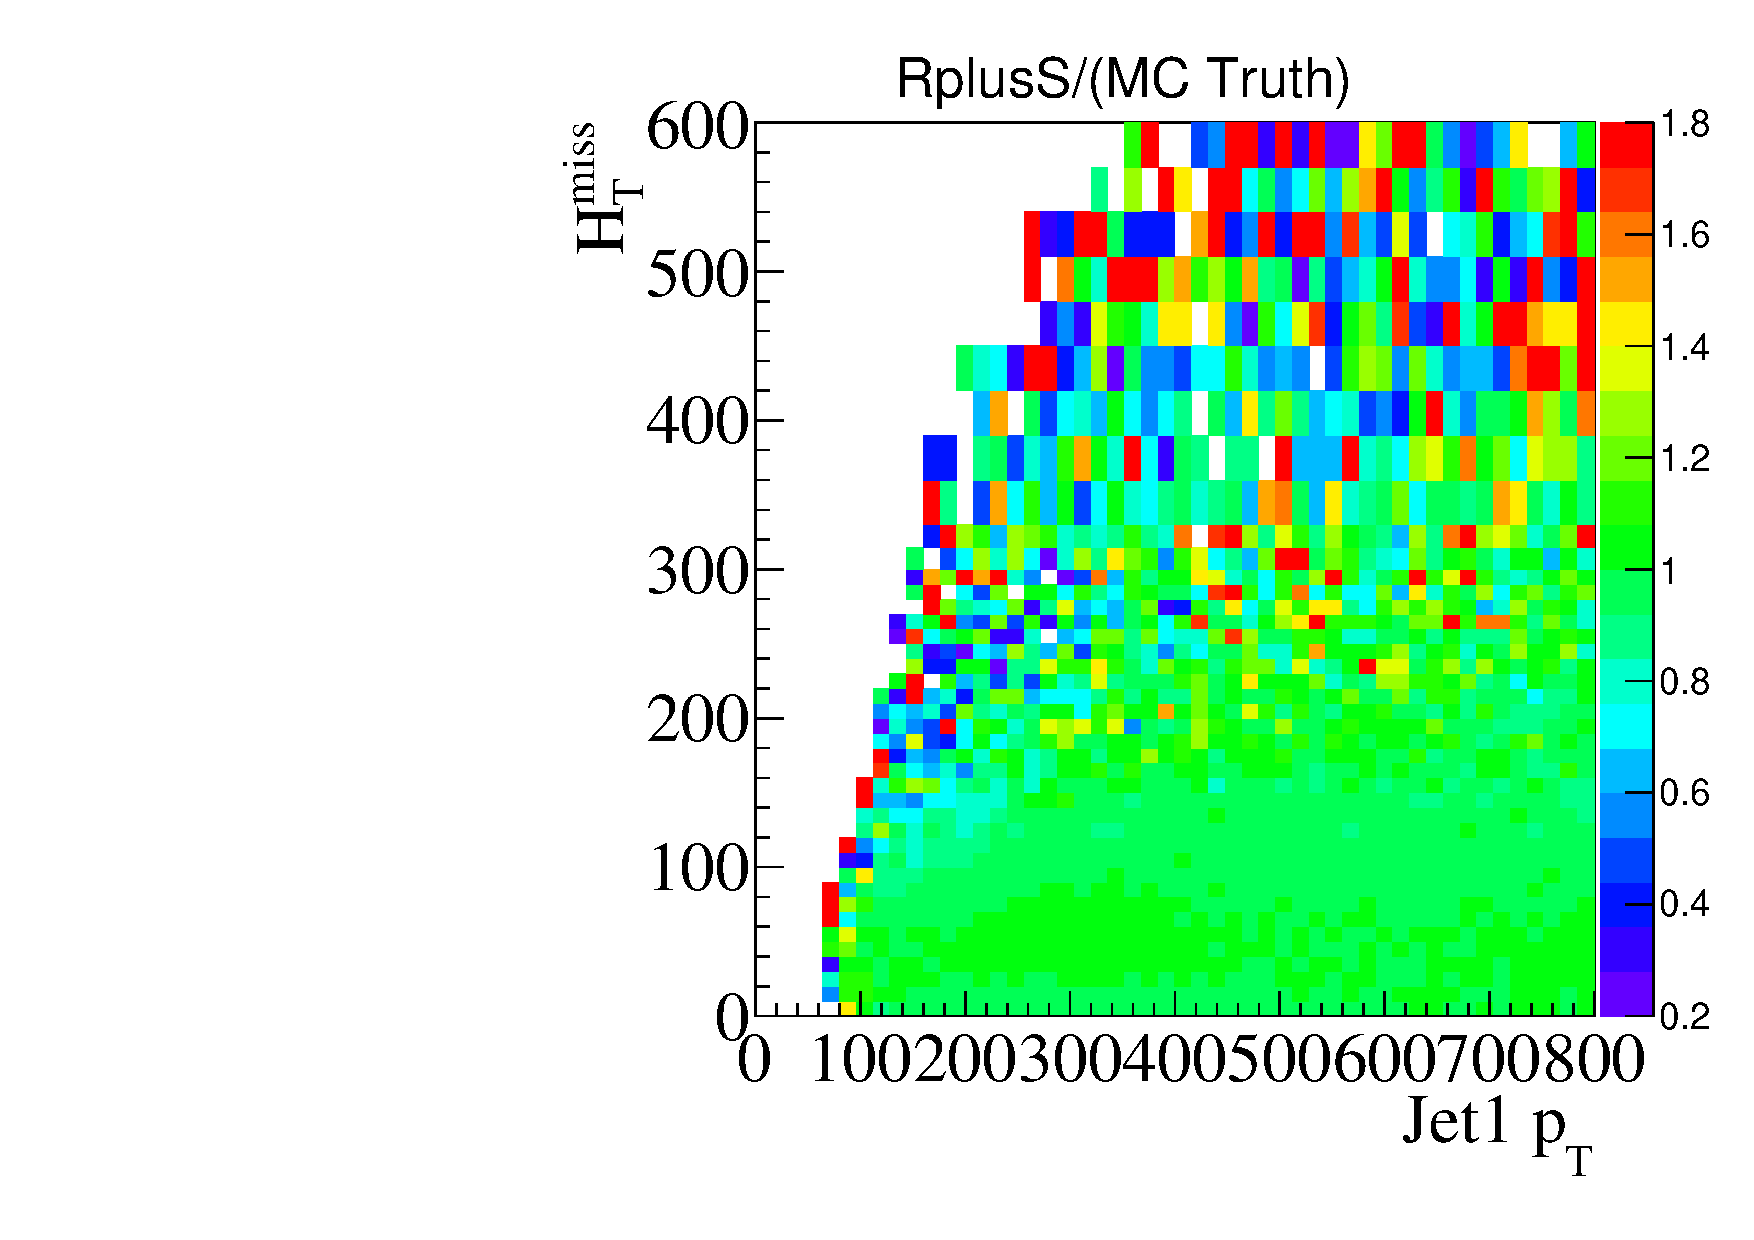
\includegraphics[width=0.5\linewidth]{figures/SusySearches/Ra2b2016/RplusSAndTruth_MhtVsJet1Pt.pdf}
}
\subfloat[]{
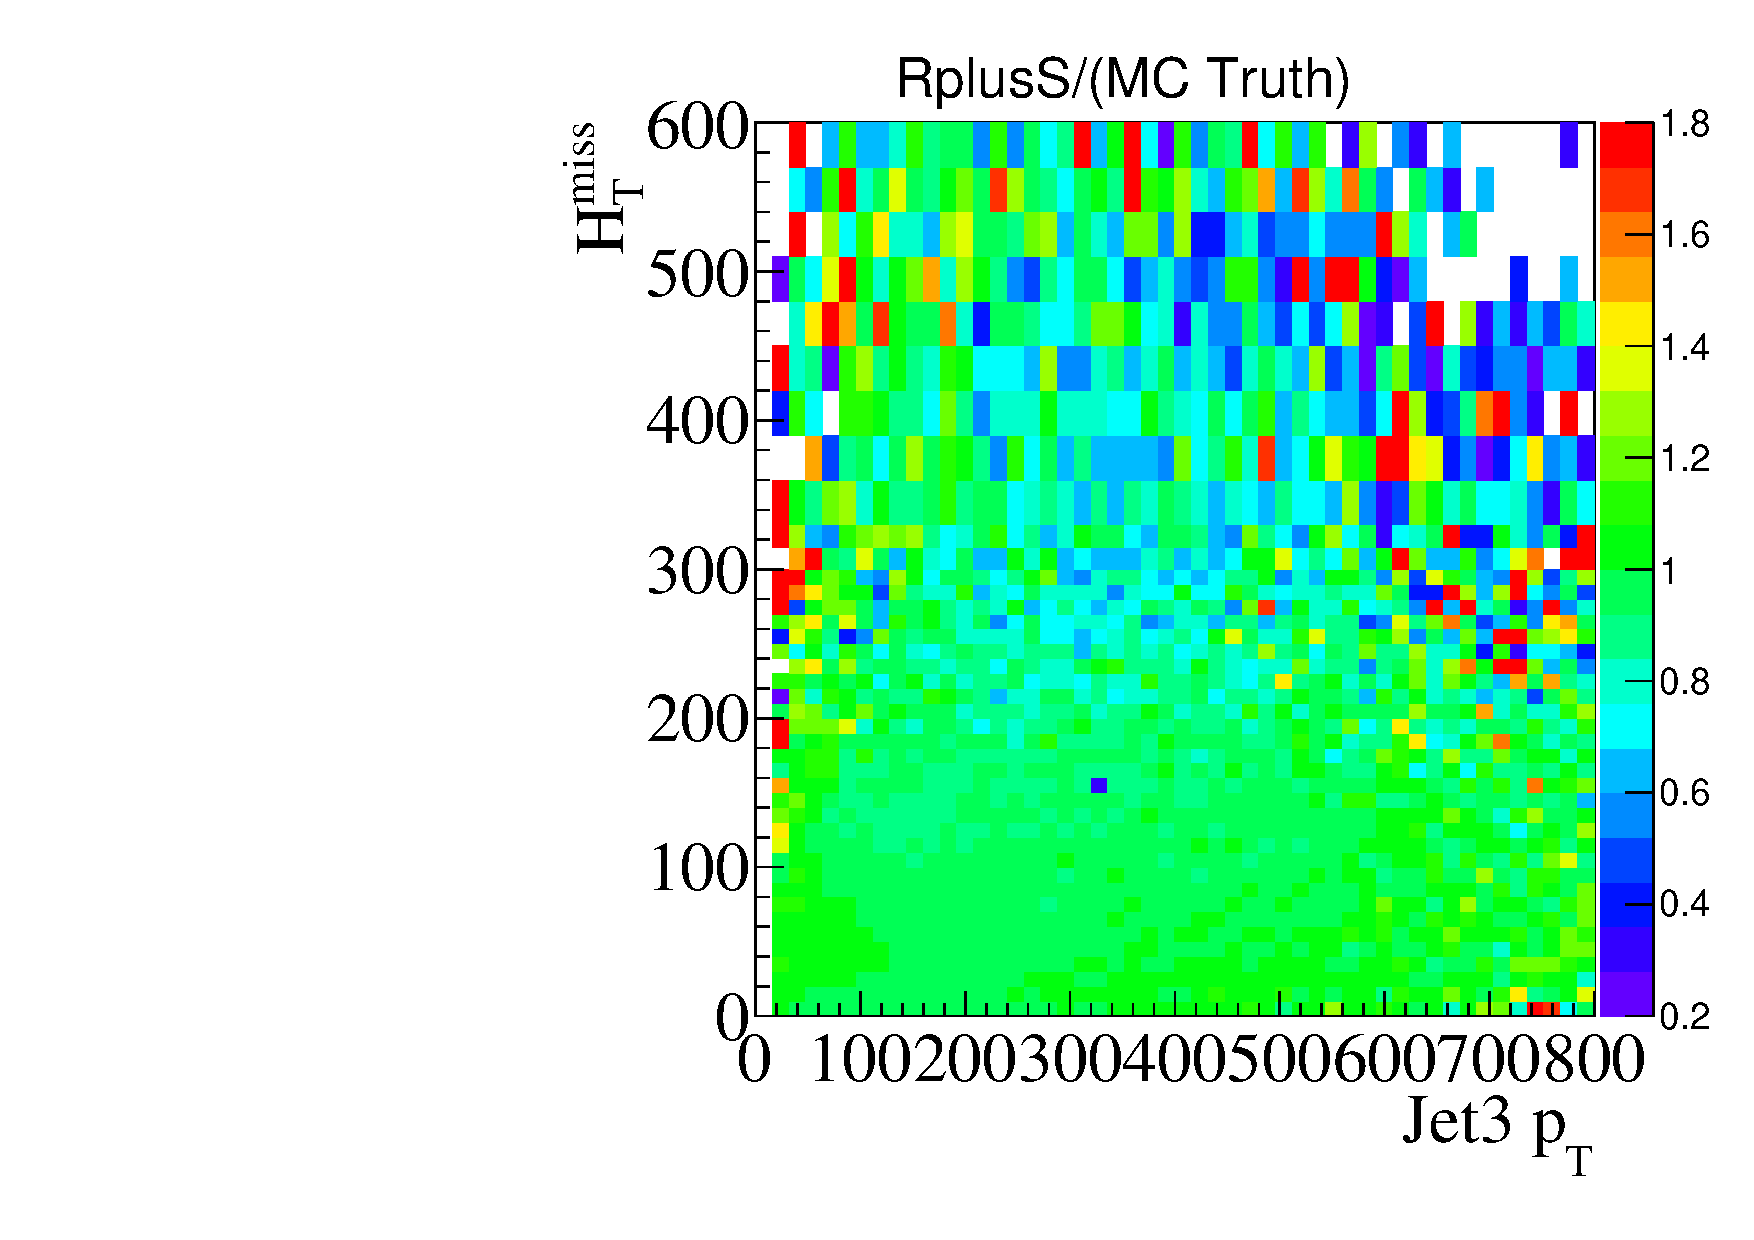
\includegraphics[width=0.5\linewidth]{figures/SusySearches/Ra2b2016/RplusSAndTruth_MhtVsJet3Pt.pdf}
}
\caption{The ratio of scatter plots of key observables for hadronic SUSY searches between the direct simulation and the rebalance and smear method applied to simulation.}
\label{fig:RplusSCorrelation}
\end{figure}
\FloatBarrier
\noindent
The degree of consistency between the prediction and the expectation in most distributions represents a significant step for QCD modeling. Not only are the relevant 1-dimensional distributions accurately modeled, but all examined pairwise correlations of the kinematic observables show acceptable closure. This includes correlations between the directions and magnitudes of the momenta of jets within an event, as well as relationships between the directions of the $\mht$ and the jets, and the magnitudes of the $\mht$ and $\Ht$. The most significant exception to these statements is with the distribution of the multiplicity of b-tagged jets,  where non-closure is evident for events with $\geq 3$ b-jets on the order $\approx50\%$. A possible source of this discrepancy is the choice of binning for the parton-level $\mht$ templates that constitute the prior, namely, $\nbjets=$ 0, 1, and $\geq$ 2.  A modification of this choice to include templates for the individual bins of $\nbjets=$ 2, 3, and $\geq 4$ may lead to improved results in the region of large b-jet multiplicity. 

The method is ready to be applied to the data, but the results are saved for the summary of the CMS hadronic multi-jet analysis, given in Section \ref{sec:ra2b2015}. I conclude for the moment with a summary of the key developments.

\subsubsection{What were the key developments?}
It appears to be feasible to use of correlations among jets in QCD events as a means of achieving signal-background discrimination in kinematic regions dominated by QCD, such as the regions of low-$\mht$ and low $\Ht$. The possibility of applying the method in the low-$\mht$ region is for the first time feasible, since the classical method does not accurately model the QCD kinematics in this region (see Fig. \ref{fig:OldVsNew}). 
\begin{figure}[h]
\centering
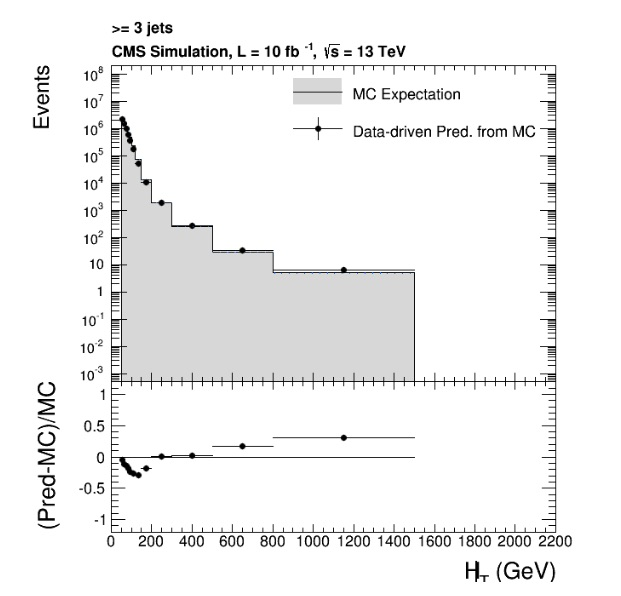
\includegraphics[width=0.49\linewidth]{figures/SusySearches/Ra2b2016/RnSClassicMht.jpg}
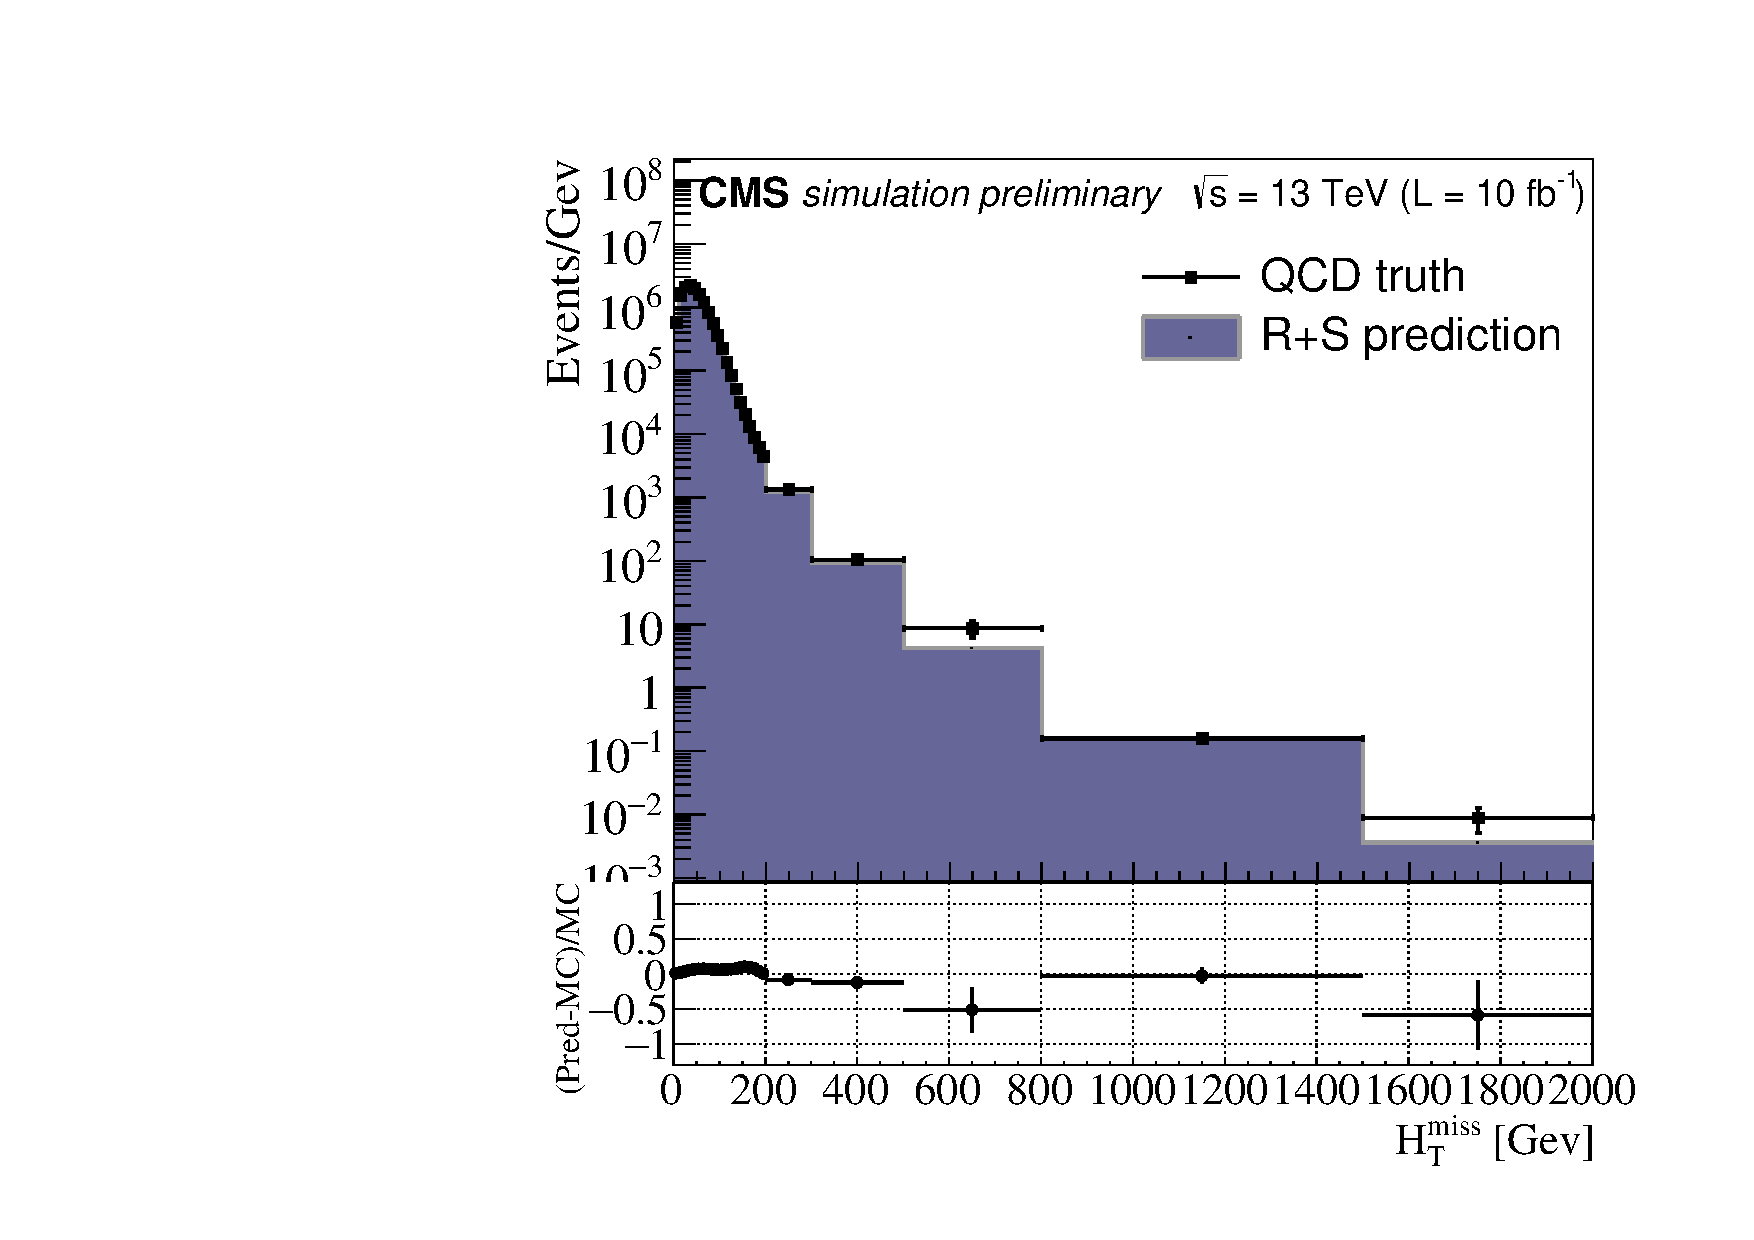
\includegraphics[width=0.49\linewidth]{figures/SusySearches/Ra2b2016/LowDeltaPhi_MhtForComparison.pdf}
\caption{Comparisons of the $\mht$ distribution between prediction and expectation using the classical method (left) and the new method (right).}
\label{fig:OldVsNew}
\end{figure}
The primary reasons for these improvements with respect to the classical method are that a realistic parton-level $\mht$ constraint is used in the rebalance procedure, whereas, in the classical method, every event is rebalanced to an $\mht$ of 0 or a constant value chosen by the user, amounting to a delta function constraint. Second, the full jet response has been used in the likelihood maximization, rather than gaussian approximations. Gaussian approximations can lead to mis-modeling of the jet $\pt$ or $\mht$ spectrum in events containing jets with small $\pt$, which exhibit a highly non-Gaussian response. 

The rebalance and smear method is robust against contamination from signal events in the prediction sample. The reason is that the rebalance procedure displaces signal-like, high-$\met$ events from the high-$\met$ region, to regions of low-$\met$; after smearing, the proportion of events in the high-$\met$ region truly originating from QCD processes is nearly 100\% (see Fig. \ref{fig:RplusSContamination}). 
\begin{figure}[tb!]
\centering
\includegraphics[width=0.6\linewidth]{figures/SusySearches/Ra2b2016/RplusSContam.pdf}
\caption{Signal contaimination removal. The midnight blue (and yellow) histograms show the distribution of QCD (and signal) events taken directly from simulation. The black (and red) histograms show the distributions of QCD (and signal) and after being processed by the rebalance and smear procedure. The signal has been removed from the high-$\mht$ region, leaving an accurately modeled QCD contribution.}
\label{fig:RplusSContamination}
\end{figure}
The robustness of the prediction to possible signal contamination in the control region allows for real events to be used directly for the prediction. Another strength is that the rebalanced events can be smeared an indefinite number of times, which allows for the accumulation of an indefinitely large prediction sample, computer resources permitting. Therefore, good estimates of the expected QCD event count and uncertainty can be made in extreme tails, even in regions for which no simulated QCD events are available. Alternatively, the rebalanced events can be smeared once set of times to generate a training sample of background events for a multivariate discriminant, and subsequent smearing can generate a statistically-independent prediction sample. This is further explored in Chapter \ref{chap:money}. Essentially, we have a data-driven QCD event generator.
\FloatBarrier

\subsection{Applying the method in data}
To derive the rebalance and smear prediction, data samples are collected with a series of pre-scaled $\Ht$ triggers,
\begin{itemize}
  \item \texttt{HLT\_PFHT200\_*},
    \item \texttt{HLT\_PFHT300\_*},
      \item \texttt{HLT\_PFHT350\_*},
        \item \texttt{HLT\_PFHT600\_*},
\end{itemize}
and the un-prescaled trigger,
\begin{itemize}
  \item \texttt{HLT\_PFHT800\_*}.
\end{itemize}
Events collected by these triggers are pooled into a single sample, here referred to as the $\Ht$ control sample. Events are rejected if the trigger with the highest possible $\Ht$ threshold that could have fired did not fire. This criterion ensures that the probability of an event being selected is equal to the pre-scale. Distributions of the weighted and un-weighted online $\Ht$, and un-weighted offline $\Ht$ are shown in Fig. \ref{fig:PrescaleWeights}.
\begin{figure}[tb!]
\centering
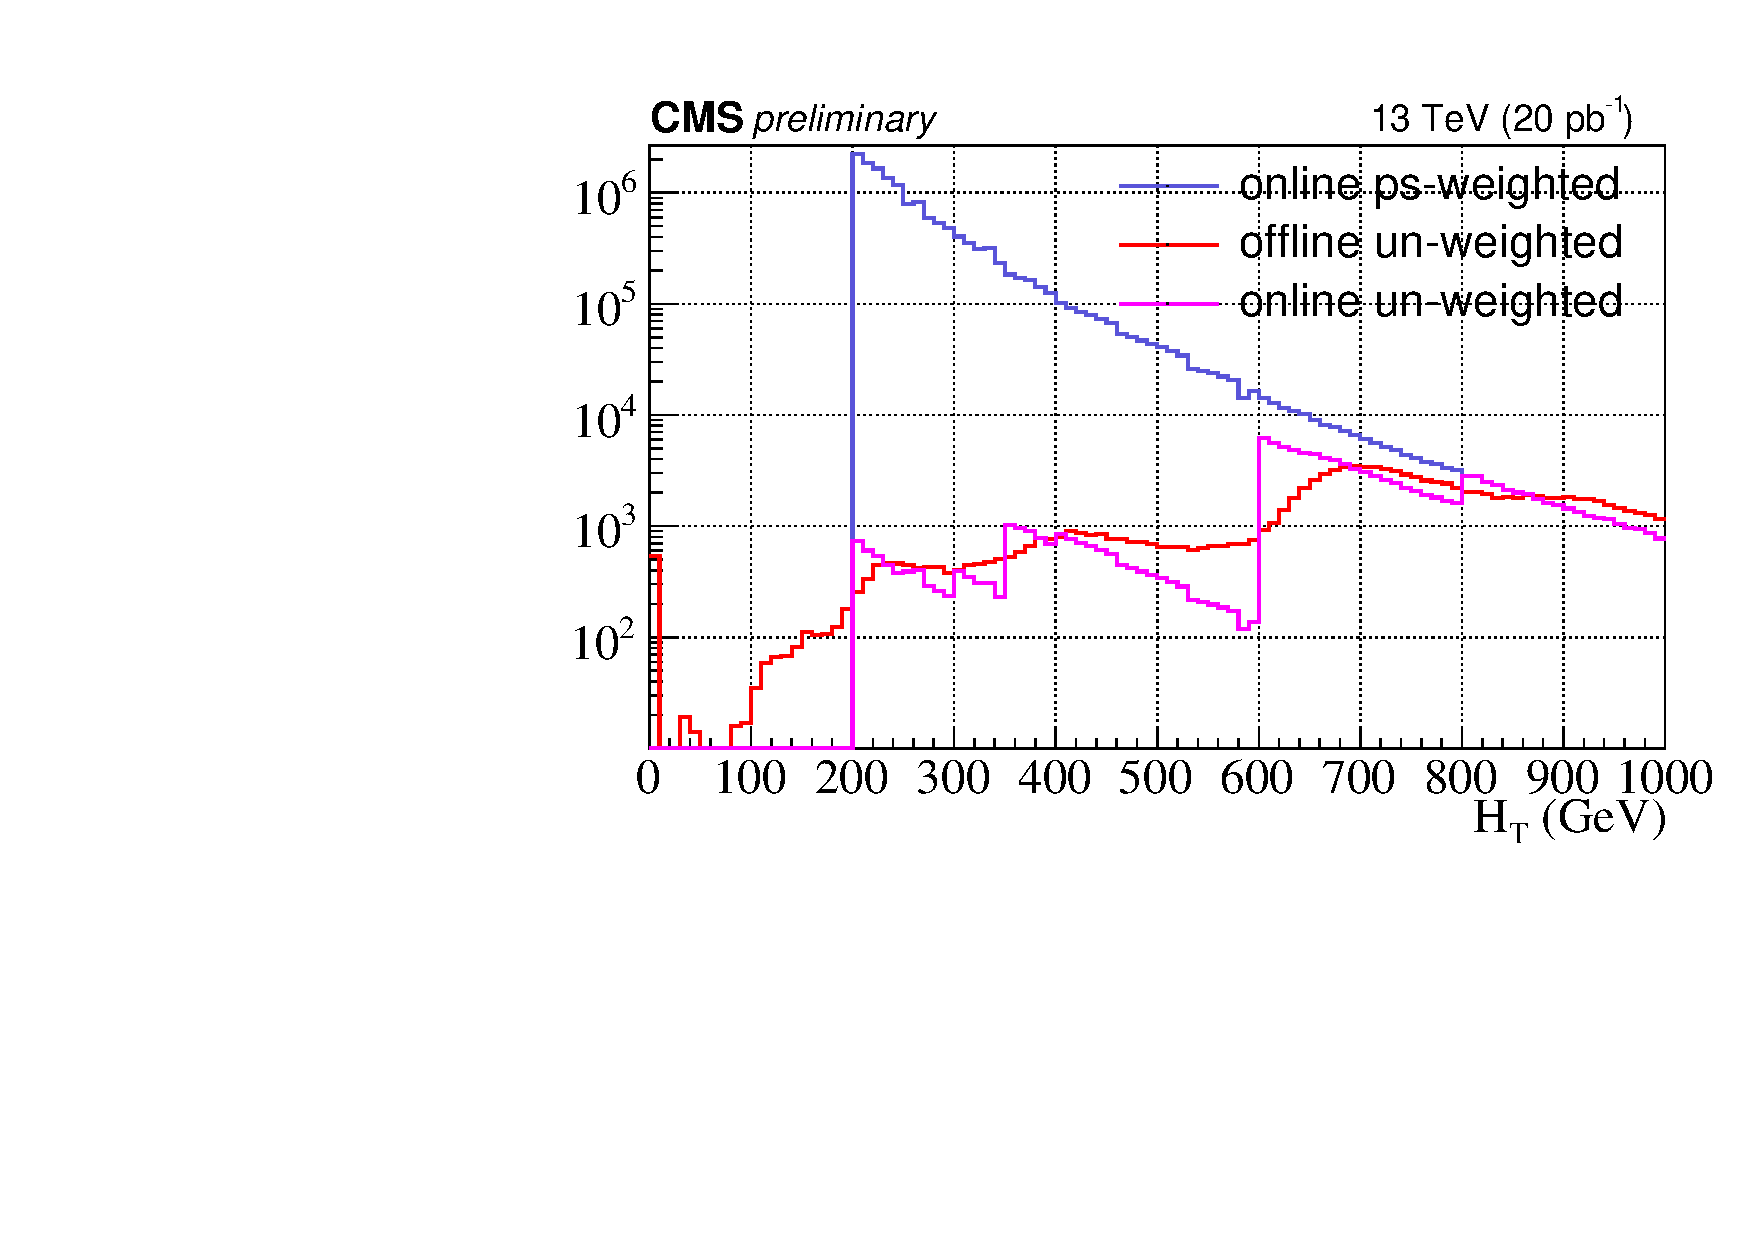
\includegraphics[width=0.6\linewidth]{figures/SusySearches/Ra2b2016/PrescaleWeightsHT2.pdf}
\caption{The distribution of the $\Ht$ in the $\Ht$ control sample for the unweighted offline $\Ht$ (red), the unweighted online $\Ht$ (pink), and the online $\Ht$ weighted by the pre-scale values.}
\label{fig:PrescaleWeights}
\end{figure}
The online pre-scale weighted $\Ht$ is smooth, as expected. The jet $\pt$ likelihoods are modified by jet resolution scale factors, derived by the jet/$\met$ POG \cite{jetmet2} to ensure the compatibility of the smearing with the true jet resolution. Rebalanced events are smeared a number of times proportional to the event's pre-scale value, which serves to apply the pre-scale weight, and ensures that all prediction events have equal weight.

\subsection{Uncertainties in the prediction}
Uncertainties in the final prediction include statistical uncertainty in the prediction, statistical uncertainty associated with the $\Ht$ control sample, uncertainty in the jet energy resolution, uncertainty in the parton-level $\mht$ prior density, and uncertainty corresponding to any non-closure. 

The statistical uncertainty in the prediction is the poisson uncertainty in the weighted number of counts in each bin. This uncertainty can, in principle, but reduced to arbitrarily small values by increasing the number of smearing trials. Given independent search regions, statistical uncertainties are uncorrelated across bins. 

The statistical uncertainty in the control sample is evaluated by making the prediction once using the entire data set, and once having randomly discarded half the control sample events. Scaling the half-discarded prediction up by a factor of two and taking the discrepancy with the original prediction yields a bin-by-bin systematic uncertainty. Uncertainties are once treated as uncorrelated across all bins.

The uncertainty in the jet energy resolution is evaluated by taking the difference between the nominal prediction and the prediction obtained by modifying the jet $\pt$ likelihoods according to the jet energy resolution uncertainties provided by  \cite{jetmet2}. Rather than evaluating the bin-by-bin discrepancy, the discrepancy in the inclusive $\mht$ distribution integrated over the bounds of each signal region between the nominal and modified predictions is taken as a percent uncertainty. This methods ensures that statistical uncertainties are not duplicated based on the limited statistics of the control sample. Uncertainties are taken to be fully correlated across all bins.

Uncertainty in the $\mht$ prior is evaluated in an analogous way as the previous uncertainty, except the difference in predictions is that between the nominal prediction and the prediction made with a modified $\mht$ prior density. The modified prior density is obtained by reweighting the nominal $\mht$ prior by the ratio of the of real reconstructed $\mht$ to the simulated reconstructed $\mht$ in the region between the values of $\mht=0$ and 200 GeV in a QCD-enriched kinematic region. The weights are order 1 with negligible uncertainties. Uncertainties are treated as correlated across bins.

An uncertainty of 50\% is assigned to search bins with greater than 2 b-tags to accommodate the non-closure in simulation. In the future, this uncertainty may be eliminated by modifying the binning of the prior template as prescribe in the previous section. Non-closure uncertainties are treated as uncorrelated across bins. 

The values of the uncertainties, along with the bin-by-bin prediction, for the multi-jet$+$$\mht$ SUSY search are given in Section \ref{sec:2015results}.



\section{Z$\rightarrow\nu\bar{\nu}$ background estimation}
\label{sec:zinv}
Events in which $Z$ bosons are produced in association with jets account for a large fraction of the high-$\met$ all-hadronic events at the LHC. Not surprisingly, these events are a major background to new physics that may manifest signals in the hadronic channel. Since the jet multiplicity beyond 4 jets, as well as the relationships between the directions of jets, are not simulated accurately, it is generally advisable to employ data-driven methods for $\zinv$ background estimation, especially when the signal region is populated by events with several jets. Typically, data-driven approaches make use of similarities between the kinematics of $\zinv$ events and $Z\rightarrow X\bar{X}$ events, where $X$ is one of the other $Z$ boson decay products, or of the similarities between events with $Z$ bosons and events with photons. The former technique is described in the following.


\subsection{The relationship between $\zinv$ and $\zll$}
The kinematics of $Z$ bosons are independent of the decay mode of the $Z$ boson, as is the case for any particle that can undergo a variety of decays. The decay modes and branching fractions $\mathcal{B}$ for the $Z$ boson are listed in Table \ref{tab:zdecay}. 

\begin{table}[h]
\vspace{0.5cm}
\centering
\begin{tabular}{l|rl}
\hline
decay mode & \multicolumn{2}{c}{$\mathcal{B}$(\%)}\\
\hline
e$^+$e$^-$ & $3.363$&\hspace{-3mm}$\pm \hspace{1mm}0.004$\\
$\mu^+\mu^-$ & $3.366$&\hspace{-3mm}$\pm \hspace{1mm}0.007$\\
$\tau^+\tau^-$ & $3.370$&\hspace{-3mm}$\pm \hspace{1mm}0.008$\\
$\nu\bar{\nu}$ & $20.00$&\hspace{-3mm}$\pm \hspace{1mm}0.06$\\
q$\bar{\text{q}}$ & $69.91$&\hspace{-3mm}$\pm \hspace{1mm}0.06$\\
\hline
\end{tabular}
\caption{The measured decay modes of the $Z$ boson, as reported in \cite{Agashe:2014kda}.}
\label{tab:zdecay}
\end{table}

Events featuring the $\zinv$ decay mode are largely indistinguishable from other events with $\met$ and no leptons, and therefore obtaining a reasonably pure data sample of $\zinv$ events is not feasible. However, events with $\zll$ decays can be selected with high purity by requiring two opposite-sign, same-flavor, well-isolated leptons, whose invariant mass falls within a range similar to $|m_{ll}-m_\text{Z}|<20$ GeV. For events in such a sample, the $Z$ boson can be reconstructed by summing the four-vectors of the two leptons, and if the $Z$ is removed from the event, a proxy sample for real $\zinv$ events is obtained. The process of removing the tagged $Z$ boson is referred to as event cleaning. 

The resulting ``cleaned'' event sample is expected to exhibit {\it all} the characteristics of the real $\zinv$ events, barring two exceptions: first, distributions of extensive properties derived from the $l\bar{l}$ sample will be too low by an overall normalization factor of $20/3.4\approx5.9$ because of the difference in branching fractions of the $\zinv$ and $\zll$ decay modes; and second, the shapes of distributions based on the $\zll$ sample will be altered because the acceptance, reconstruction efficiency, and isolation efficiency of the lepton selection. To correct for the first difference, $\zll$-derived distributions are scaled up by the normalization factor 5.9. To correct for the second difference, events in the $\zll$ sample are weighted by the inverse of the lepton efficiencies mentioned. The prediction for the $\zinv$ count $N_i$ in a given signal region $i$ is therefore given by
\begin{equation}
N_i = N_i(\zll)\cdot\frac{1}{\epsilon^{\text{Z}}_{\text{acc}}}\cdot\frac{1}{\epsilon^{\text{Z}}_{\text{rec}}}\cdot\frac{1}{\epsilon^{\text{Z}}_{\text{iso}}}\cdot\frac{\mathcal{B}(\zinv)}{\mathcal{B}(\zll)},
\label{eq:zinv}
\end{equation}
where $N_i(\zll)$ is the observed count in signal region $i$ from the cleaned dilepton sample, and the $\epsilon^{\text{Z}}$'s are the efficiencies of acceptance, reconstruction, and isolation.

\subsection{Procedure with 13 TeV data} 
A procedure was developed previously \cite{CMS:2016nhb} to estimate the $\zinv$ counts using events with two opposite-sign muons, using simulated events as well as real events collected in 2015. Muon events were chosen rather than electron events, since the muon efficiency is roughly 10\% larger than the electron efficiency, a choice that yields the larger of the two dilepton samples. However, the number of real events containing $\zmumu$ decays are limited because of the integrated luminosity recorded in 2015 is relatively small, and so an estimate of the $\zinv$ count could not be made in all signal regions. Thus, a data-simulation hybrid approach was taken, detailed in Ref. \cite{CMS:2016nhb}, in which simulated $\zinv$ events are reweighted based on the ratio of counts between data and simulation in bins of jet multiplicity and b-jet multiplicity, and are subsequently taken as the prediction. Systematic uncertainties, as well as the weights, are derived in control regions that are believed to be signal-poor; the systematic effects include those associated with the normalization uncertainty, shape uncertainties, and uncertainties associated with the reweighting. 

I developed the method to incorporate a data event sample with two opposite-sign electrons to complement, and further constrain, the $\zinv$ background prediction. On its own, the dielectron-based prediction is not expected to yield a better prediction, namely, a prediction with smaller uncertainties, than the dimuon-based prediction; however, given that electron and muon efficiencies are comparable within about 10\%, the combination of dimuon and dielectron data should result in a reduction in control region statistical uncertainties by $\approx$ 30\%. 

Reconstructed electrons are selected with $\pt$ greater than 33 (36) GeV, a threshold chosen to ensure the double electron trigger,
\begin{itemize}
  \item \texttt{HLT\_DoubleEle33\_CaloIdL\_GsfTrkIdVL\_MW\_v},
\end{itemize}
has a nearly 100\% probability of selecting electrons passing the selection, and $|\eta|$ less than 2.5. Electrons are also required to be isolated.  An isolated electron has an isolation value less than 0.1,  where isolation is defined as the ratio of the $\pt$ sum of reconstructed particles within a $\Delta R$ cone around the lepton (excluding the lepton) to the $\pt$ of the lepton, where the cone size R varies with the the lepton $\pt$:
\begin{equation}
\text{isolation} = \sum_{i}(p_{T})_i \cdot \Theta[R^*-\Delta R_{i})]/(p_T)_{\text{lepton}},
\label{eq:isolation}
\end{equation}
\[
R^* = 
  \begin{cases} 
  0.2 & \text{: } \pt \leq 50 \text{ GeV} \\
  (10 \text{ GeV})/\pt & \text{: } 50 < \pt \leq 200 \text{ GeV} \\  
   0.05 & \text{: } \pt > 200 \text{ GeV}. \\
  \end{cases}
\]
\noindent 

An essential objective is finding a suitable parametrization of the efficiencies, $\epsilon^{\text{Z}}_{\text{acc}}$, $\epsilon^{\text{Z}}_{\text{rec}}$, and $\epsilon^{\text{Z}}_{\text{iso}}$, that will result in the shapes of distributions derived from the cleaned dielectron sample agreeing with those of the $\zinv$ events. Since it is not the $Z$ bosons themselves that are reconstructed, but their decay products, a good parametrization must incorporate information about the leptons, but characterize the $Z$ boson itself.  This approach is distinct from the approach taken in the dimuon method where the efficiencies are parametrized in terms of properties of individual leptons, and the efficiencies for the two leptons in each event are multiplied to yield an event-level efficiency. The efficiency maps are now presented, based on the parametrization that was ultimately chosen. 

\subsubsection{Acceptance $\epsilon^{\text{Z}}_{\text{acc}}$}
The acceptance is defined as the fraction of $\zee$ events where both electrons satisfy the kinematic criteria
\begin{itemize}
\item $\pt>33$ GeV
\item $|\eta|<2.5$.
\item $|m_{ll}-m_{\text{Z}}|<20$ GeV
\end{itemize}
Since the $Z$ boson $\pt$ and $\eta$ are correlated with but not equal to the $\pt$ and $\eta$ of both electrons, these observables are a well-suited option for the acceptance parametrization. Figure \ref{fig:ZeeAcceptance} shows the acceptance as a function of the inferred $Z$ boson $\eta$ and $\pt$. 
\begin{figure}[tb!]
\centering
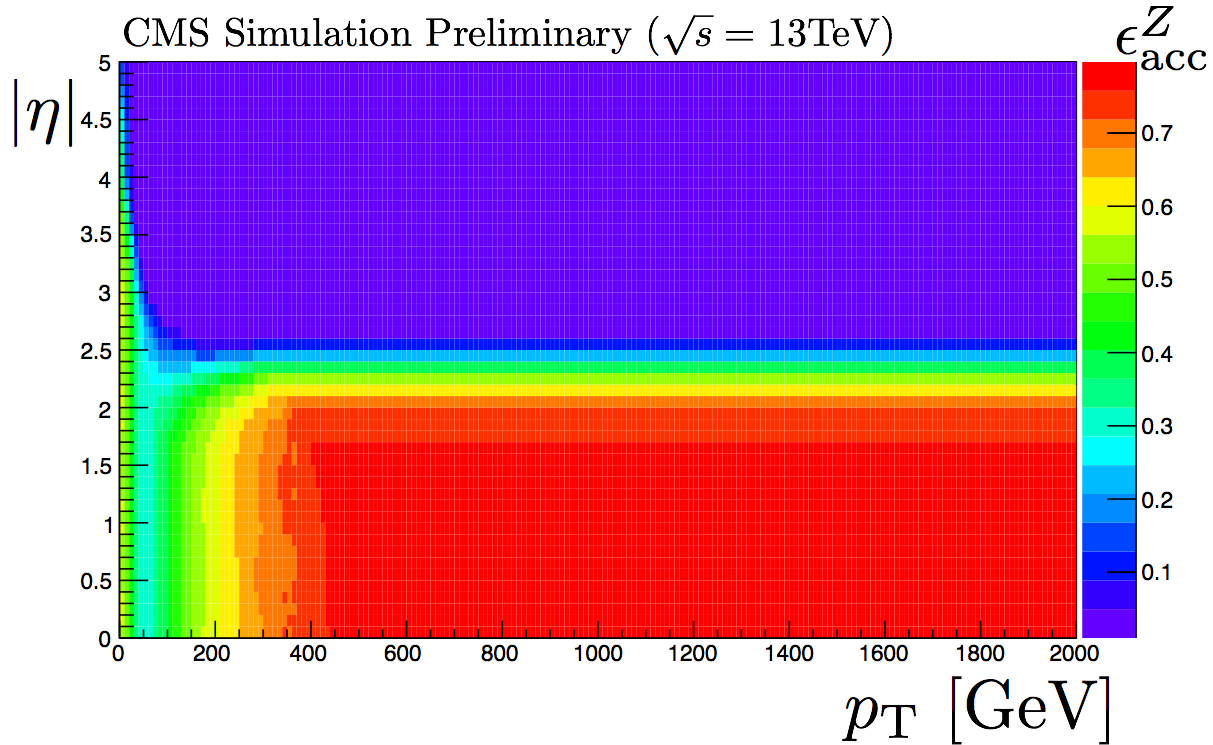
\includegraphics[width=0.7\linewidth]{figures/SusySearches/HadStop2015/ZeeAcceptance.png}
\caption{The $Z$ boson acceptance in simulated events with $\zee$.}
\label{fig:ZeeAcceptance}
\end{figure}

\subsubsection{Reconstruction efficiency $\epsilon^{\text{Z}}_{\text{rec}}$}
The reconstruction efficiency is defined as the fraction of $\zee$ events passing the acceptance criteria detailed in the previous section for which there are two reconstructed electrons in the event. The electron reconstruction is performed with the particle flow algorithm~{\cite{Beaudette:2014cea} introduced in Chapter \ref{chap:cms}. A set of selection criteria based on a recommendation by the Physics Object Group (POG) called the ``Cut Based VETO'' selection \cite{bib:ElectronID} is used, which features a very high overall electron efficiency of around 95\%. 

Since the reconstruction efficiency is expected to vary with the lepton $\pt$ and $\eta$, the $Z$ boson $\pt$ and $\eta$ are again selected as the observables used in the efficiency parametrization. Figure \ref{fig:ZeeReconstruction} shows the reconstruction efficiency as a function of the inferred $Z$ boson $\eta$ and $\pt$. 
\begin{figure}[tb!]
\centering
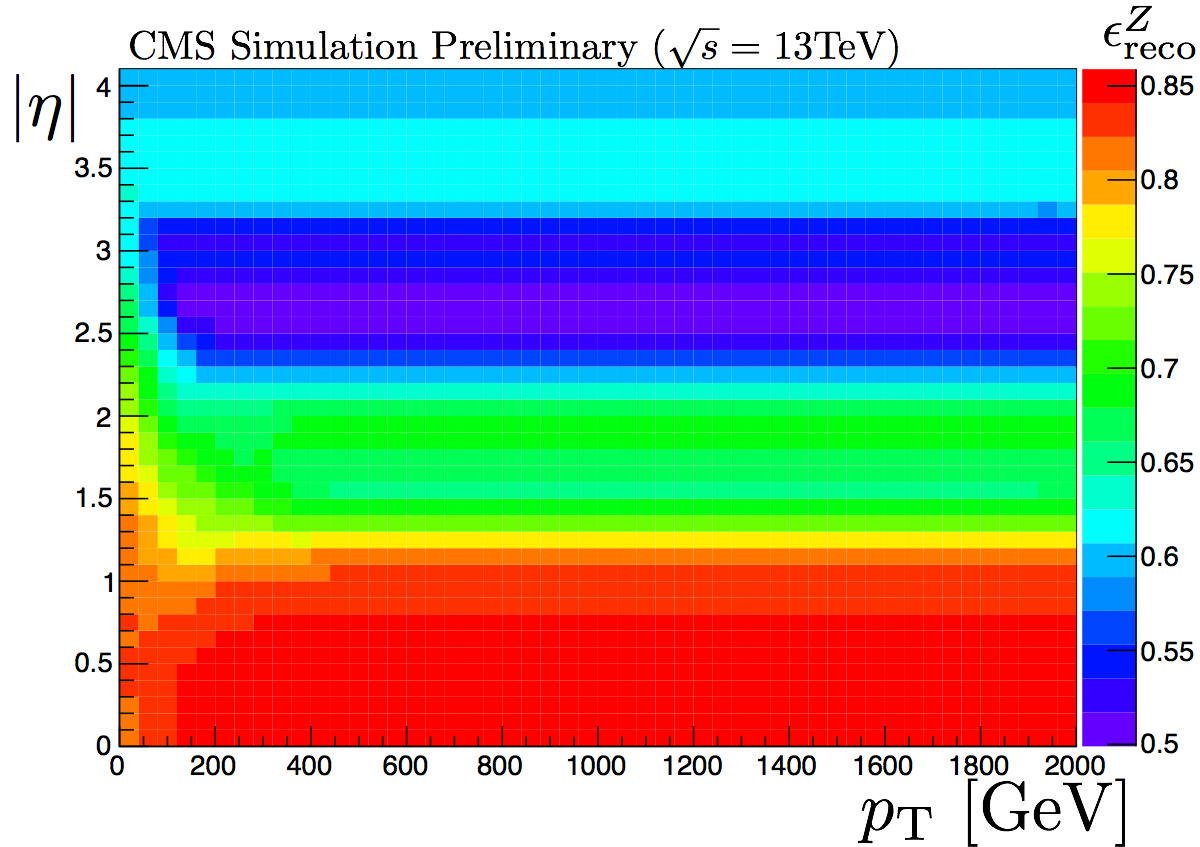
\includegraphics[width=0.7\linewidth]{figures/SusySearches/HadStop2015/ZeeReconstruction.png}
\caption{The $Z$ boson reconstruction efficiency in simulated events with $\zee$ decays.}
\label{fig:ZeeReconstruction}
\end{figure}
\FloatBarrier

\subsubsection{Isolation efficiency $\epsilon^{\text{Z}}_{\text{iso}}$}
The isolation efficiency is the fraction of $\zee$ events passing the acceptance and reconstruction criteria detailed in the previous sections for which there are two isolated electrons in the event. 

Unlike for the acceptance and the reconstruction efficiency, the isolation of the electrons is not strongly correlated with the $\pt$ or $\eta$ of the parent $Z$ boson, at least for $\pt$ values below 300 GeV. Observables that describe the $Z$ boson, but which are correlated with the electron isolation, must be constructed. There are two main effects that can cause an event to fail the isolation: first, one or both of the electrons may happen to travel in a direction collinear with jets or other particles in the event, or second, in the case of a highly energetic $Z$ boson, the electrons can be highly collinear with each other. It makes sense to parametrize the efficiency as a function of one variable that captures the effects of the first scenario, and one variable that captures those of the second. The variables chosen are the $\Delta R (\text{e}_1, \text{e}_2)$ between the two electrons, and the geometric mean of the activity of the two electrons, where the activity is defined as the $\pt$ sum of reconstructed particles in an annulus around the lepton with an inner radius of the isolation cone radius and an outer radius of 0.4, divided by the lepton $\pt$:

\begin{equation}
\text{activity} = \sum_{i}(p_{T})_i \cdot \Theta[0.4-\Delta R_{i})] \cdot \Theta[\Delta R_{i}-R^*]/(p_T)_{\text{lepton}},
\end{equation}
where R$^*$ is defined above.
Figure \ref{fig:ZeeIsolation} shows the isolation efficiency map using this parametrization. 
\begin{figure}[tb!]
\centering
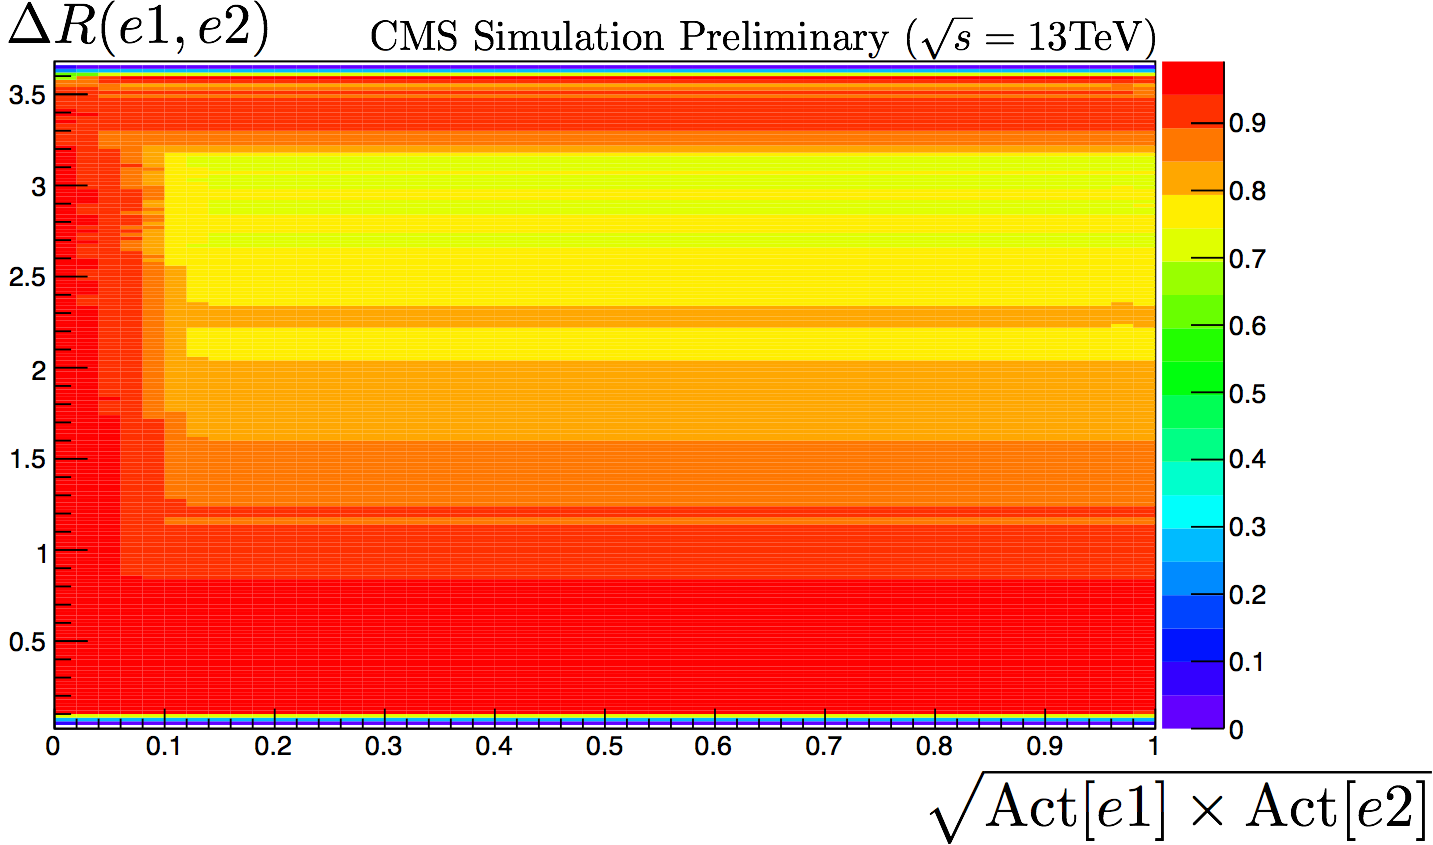
\includegraphics[width=0.7\linewidth]{figures/SusySearches/HadStop2015/ZeeIsolation.png}
\caption{The $Z$ boson isolation efficiency as a function of the $\Delta R$ between the two electrons and the geometric mean of the activities of the electrons in simulated events with $\zee$ decays.}
\label{fig:ZeeIsolation}
\end{figure}
\FloatBarrier

\subsection{Closure}
The prediction is applied to simulated $\zll$ events and compared with the result obtained directly from $\zinv$ simulation. The baseline selection of \cite{Khachatryan:2016kdk}, 
\begin{itemize}
\item no reconstructed, isolated lepton with a $\pt>10$ GeV and $|\eta|<2.4$;
\item no reconstructed, isolated particle track with a $\pt>10$ GeV and $|\eta|<2.4$;
\item $\Ht>500$ GeV;
\item $\met>200$ GeV;
\item $\Delta\phi(\mht$, jet$_{1,2,3})>$ 0.5, 0.5, 0.3;
\item $N_t\geq1$, where $N_t$ is the multiplicity of jets identified as originating from a top quark;
\item $\nbjets\geq1$, and
\item $M_{\text{T2}}>200$ GeV (see Appendix \ref{app:discriminators} for more details).
\end{itemize}
described in greater detail in the Section \ref{sec:2015results}}, is applied. Figures \ref{fig:ZInvBaseline_MetHtNjMt2} and \ref{fig:ZInvBaseline_NbNt} show the distributions for the $\zinv$ prediction using Equation \ref{eq:zinv}, the efficiencies presented in the previous section, the branching fractions quoted in Table \ref{tab:zdecay}, compared with the expectation from $\zinv$ simulation. Figures \ref{fig:ZInvCR_MetHtNjMt2} and \ref{fig:ZInvCR_NbNt} show the comparisons in the loosened baseline control region (also described in Section~\ref{sec:2015results}) in which the $\met$ and $\Ht$ selection has been relaxed.
\begin{figure}[tb!]
\centering
\subfloat[]{
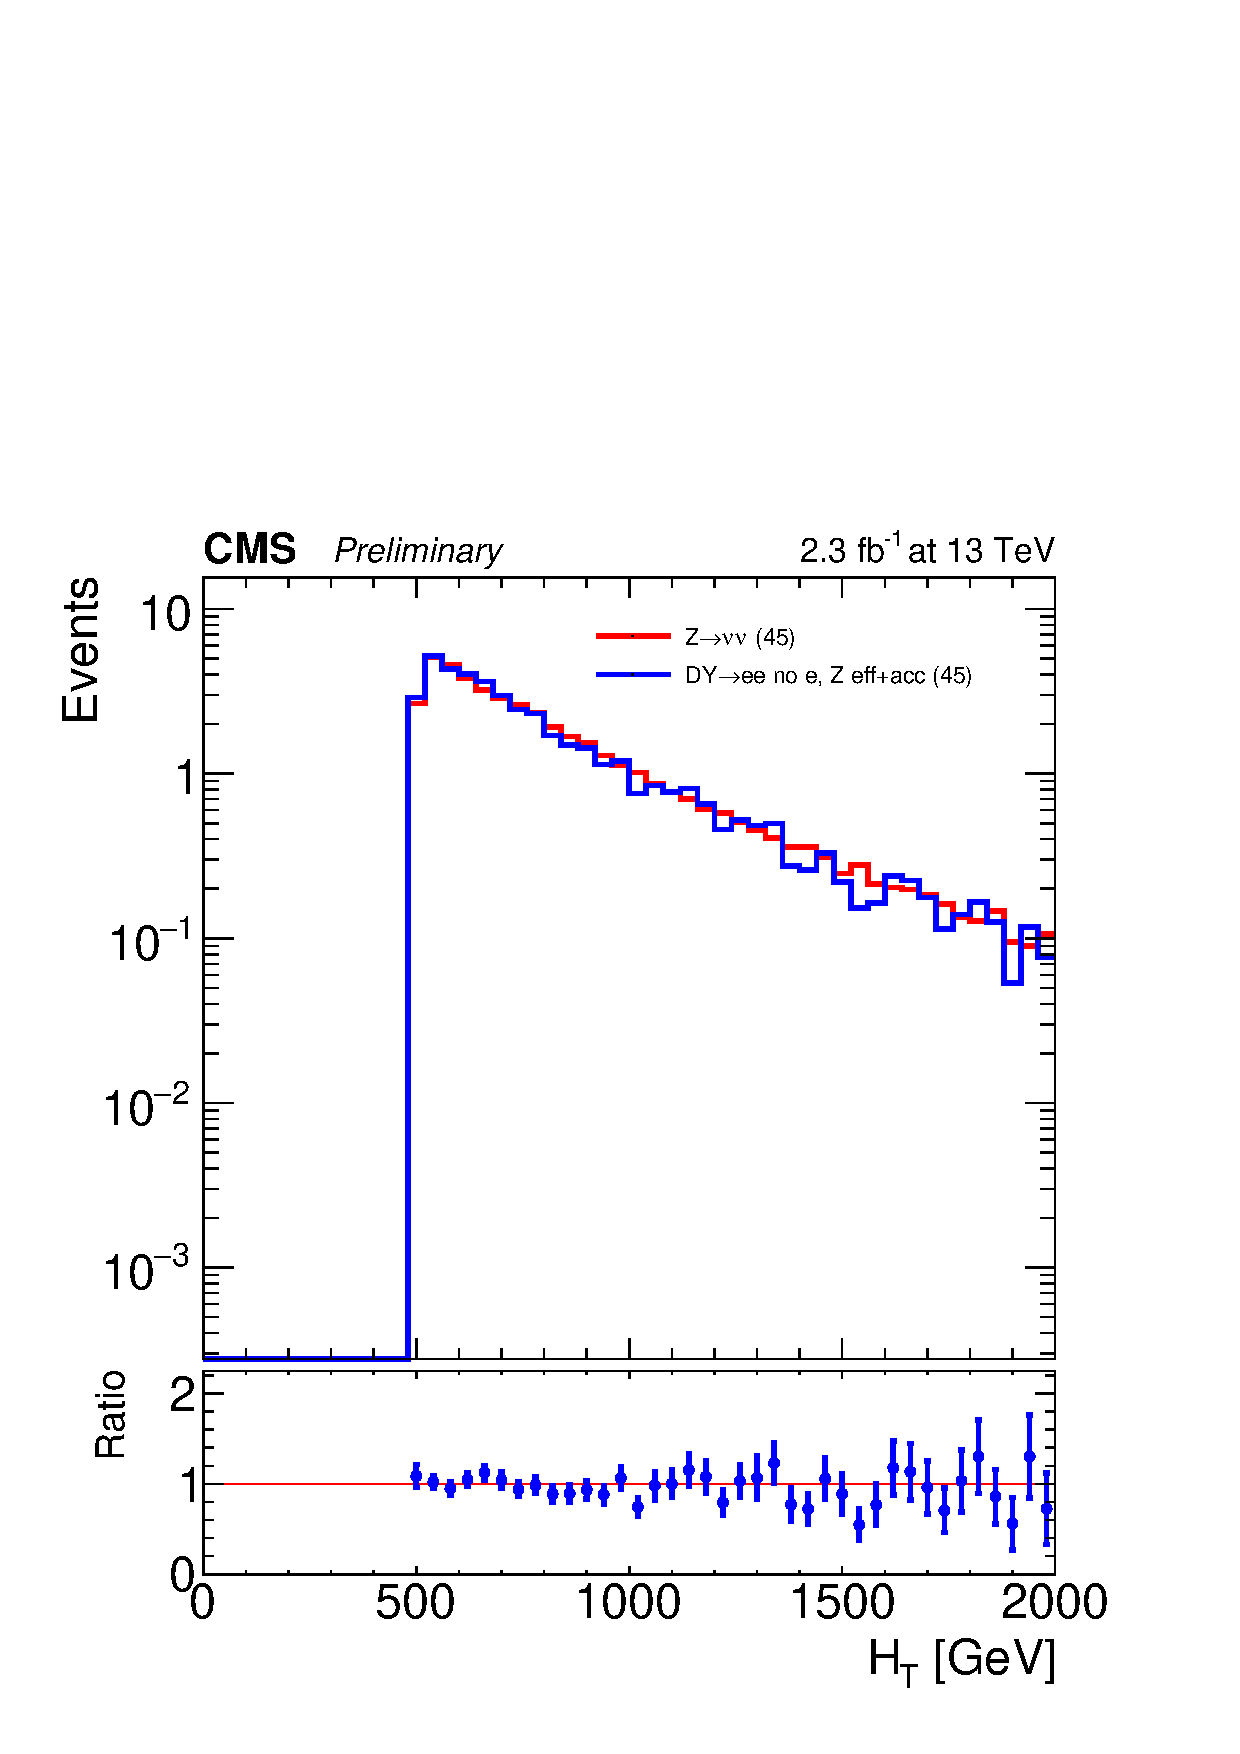
\includegraphics[width=0.5\linewidth]{figures/SusySearches/HadStop2015/MCClosure_elec_baseline_cleanht.pdf}
}
\subfloat[]{
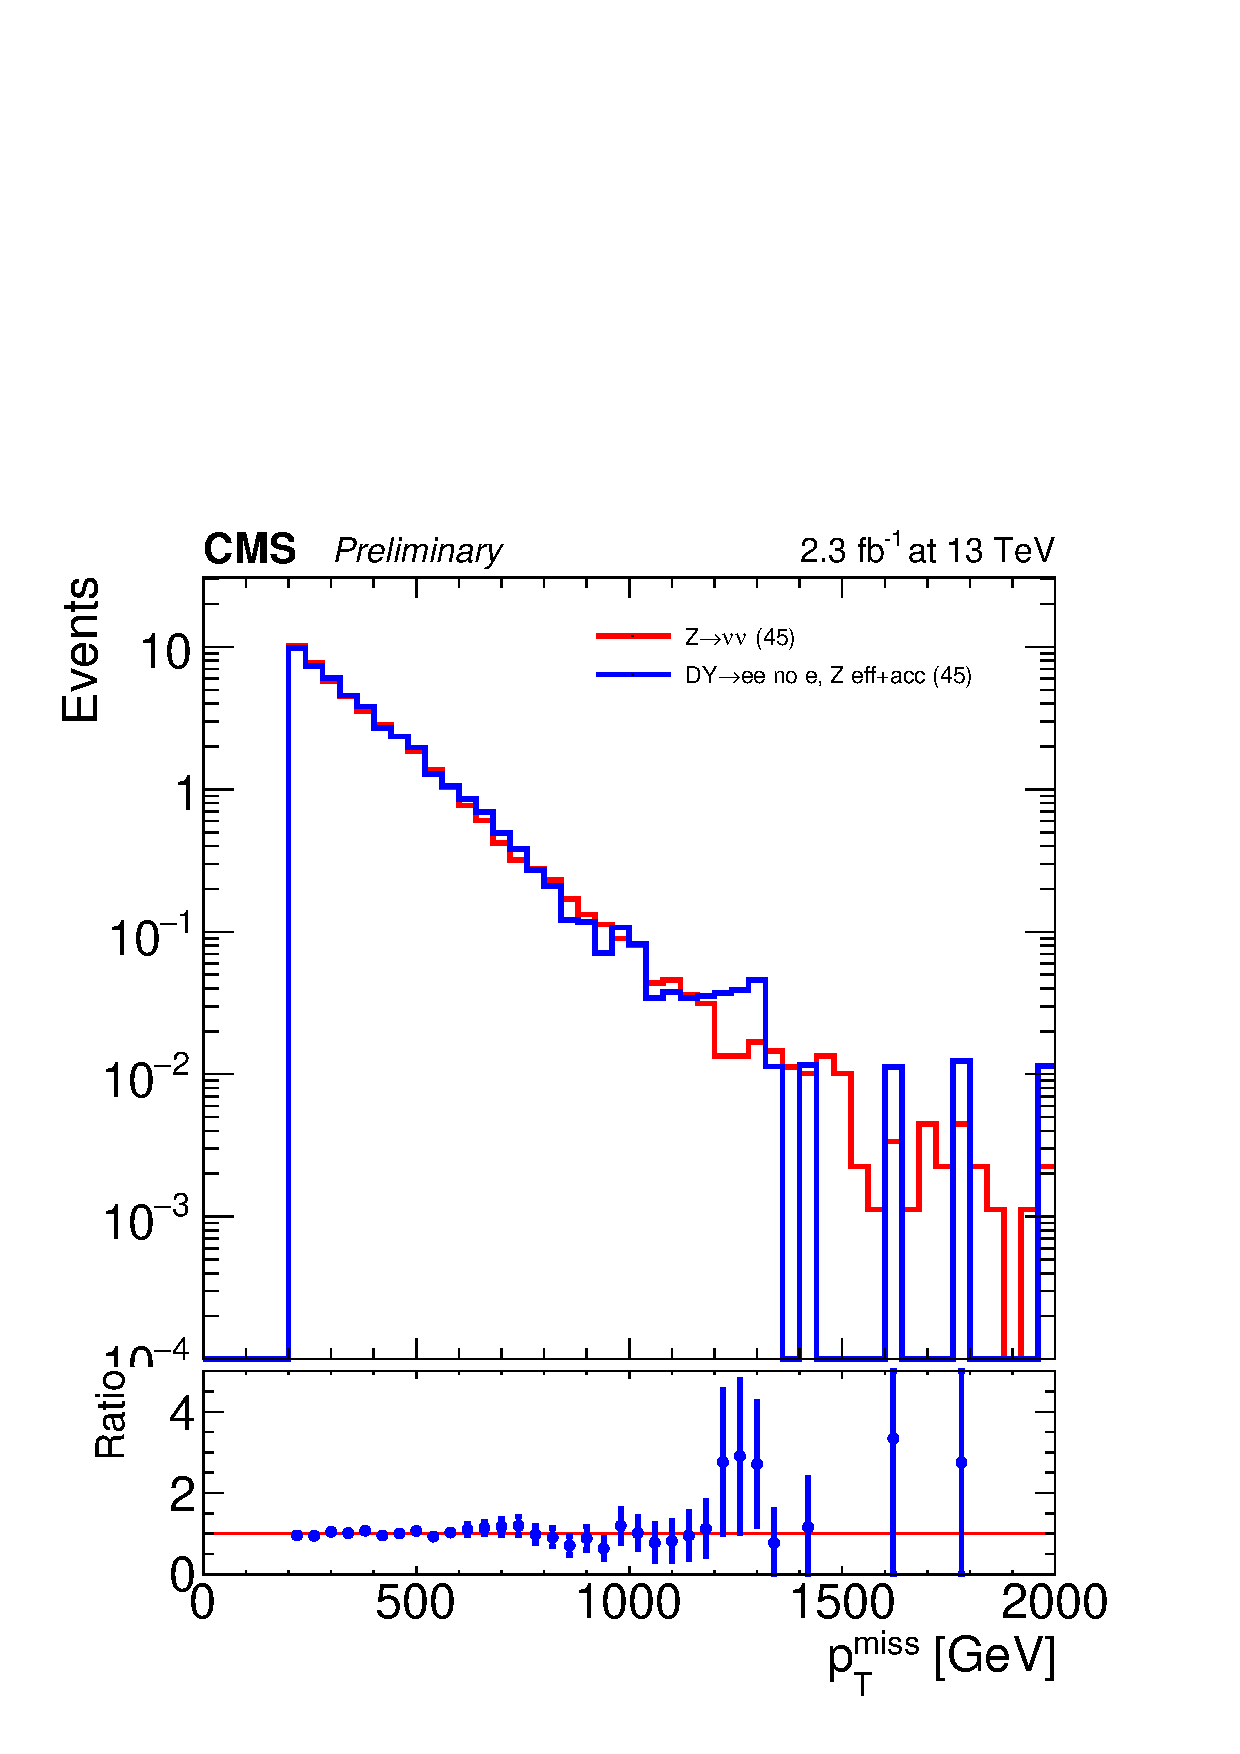
\includegraphics[width=0.5\linewidth]{figures/SusySearches/HadStop2015/MCClosure_elec_baseline_cleanmet.pdf}
}\\
\subfloat[]{
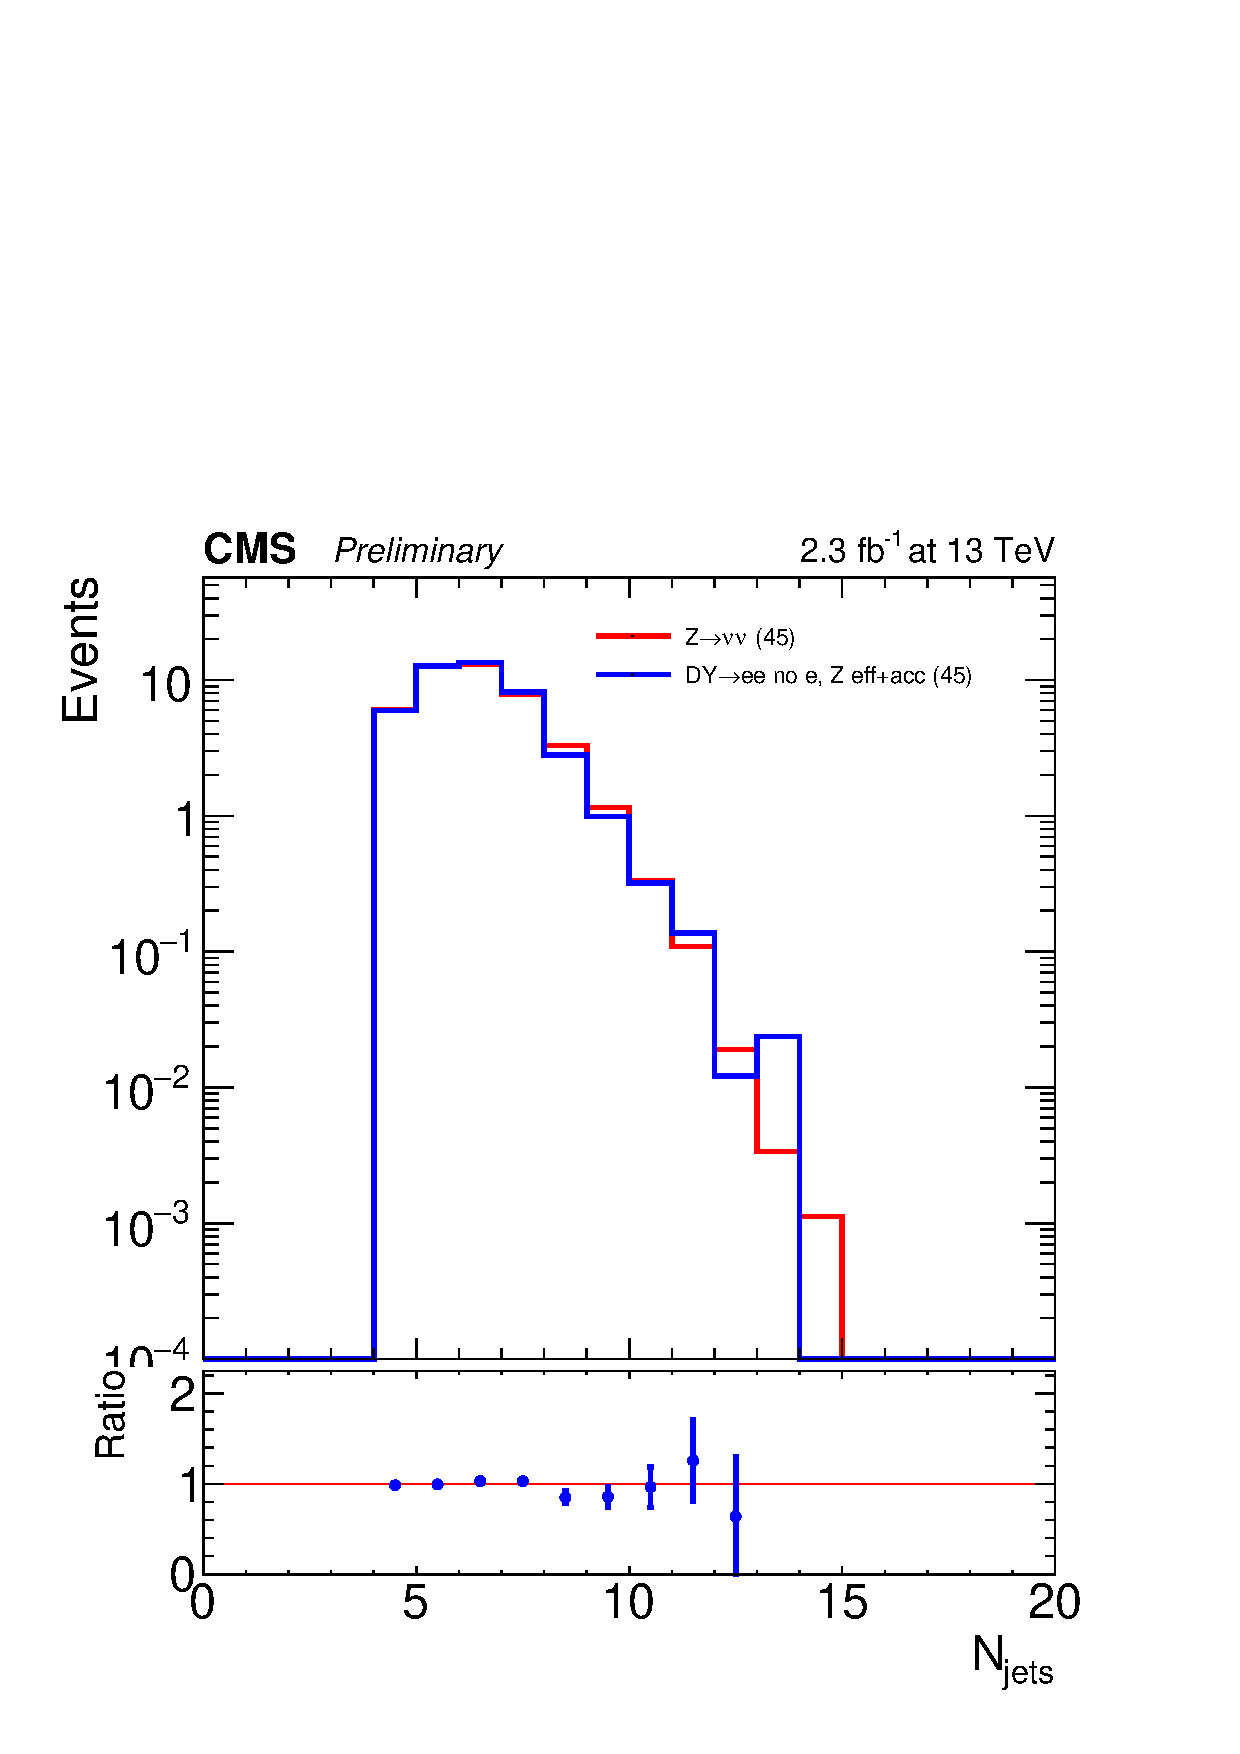
\includegraphics[width=0.5\linewidth]{figures/SusySearches/HadStop2015/MCClosure_elec_baseline_cleannJet.pdf}
}
\subfloat[]{
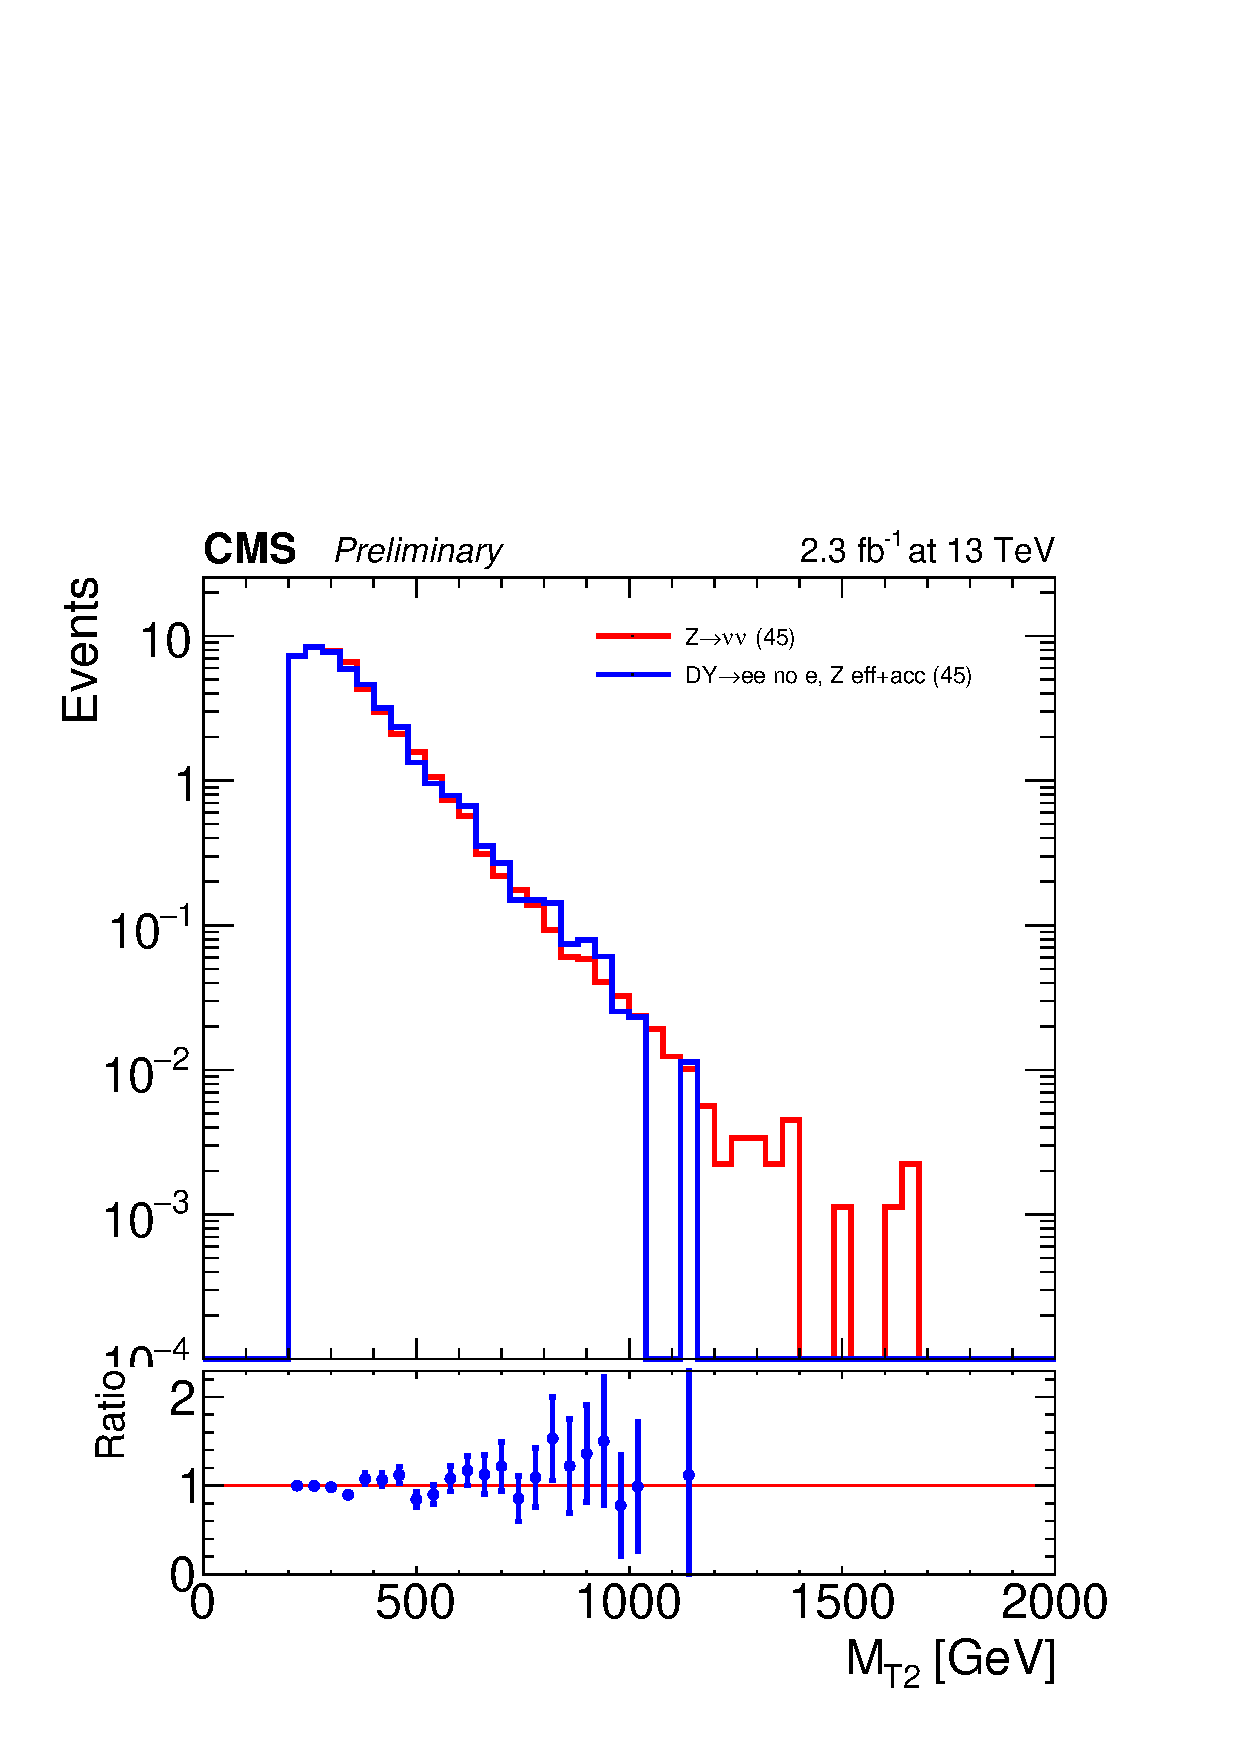
\includegraphics[width=0.5\linewidth]{figures/SusySearches/HadStop2015/MCClosure_elec_baseline_mT2Zinv.pdf}
}
\caption{Comparison of $\zinv$ prediction (blue) and expectation (red) for the $\Ht$ (1) and $\met$ (2), the jet multiplicity (3) and the $M_{T2}$ (4), after the baseline selection of the 2015 hadronic stop analysis. The ratio is of the prediction to the expectation. All events are from simulation.}
\label{fig:ZInvBaseline_MetHtNjMt2}
\end{figure}

\begin{figure}[tb!]
\centering
\subfloat[]{
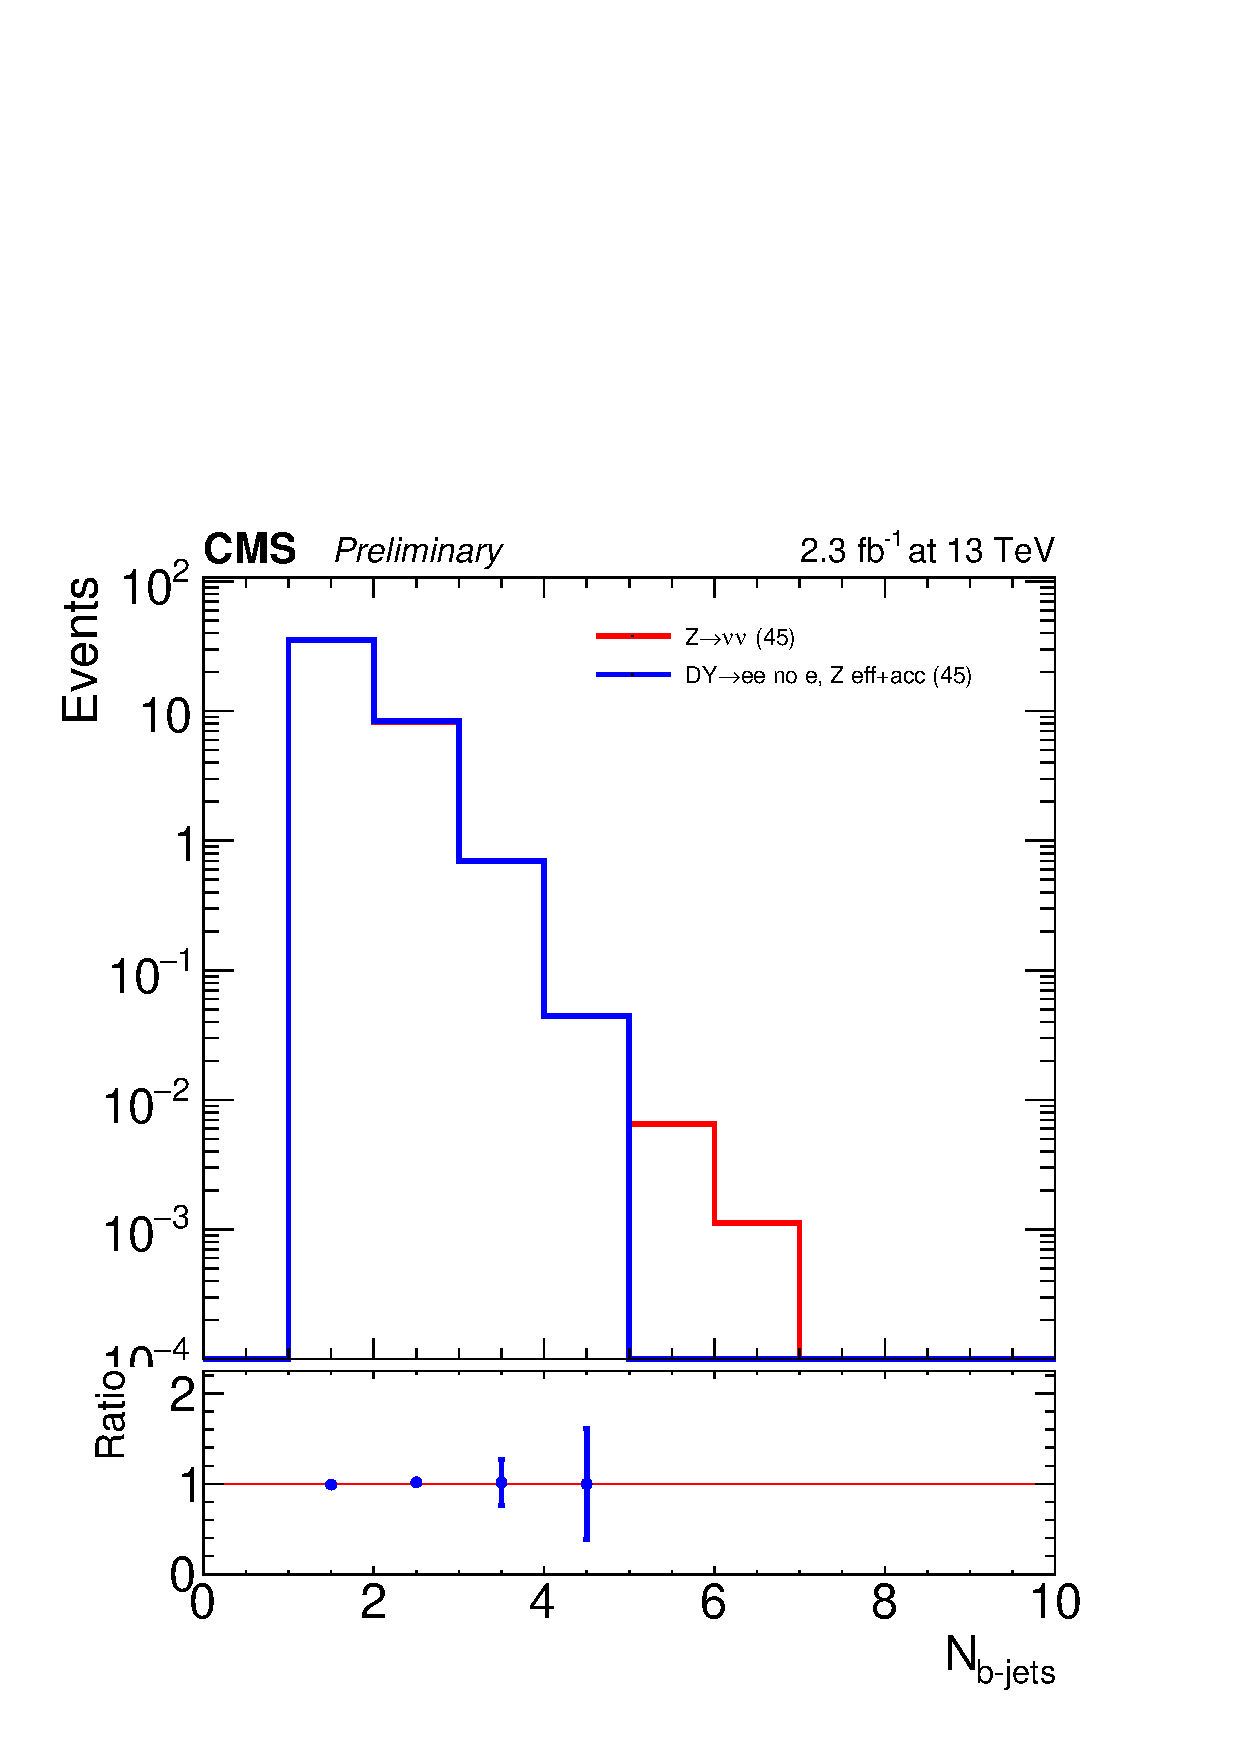
\includegraphics[width=0.5\linewidth]{figures/SusySearches/HadStop2015/MCClosure_elec_baseline_nBottom.pdf}
}
\subfloat[]{
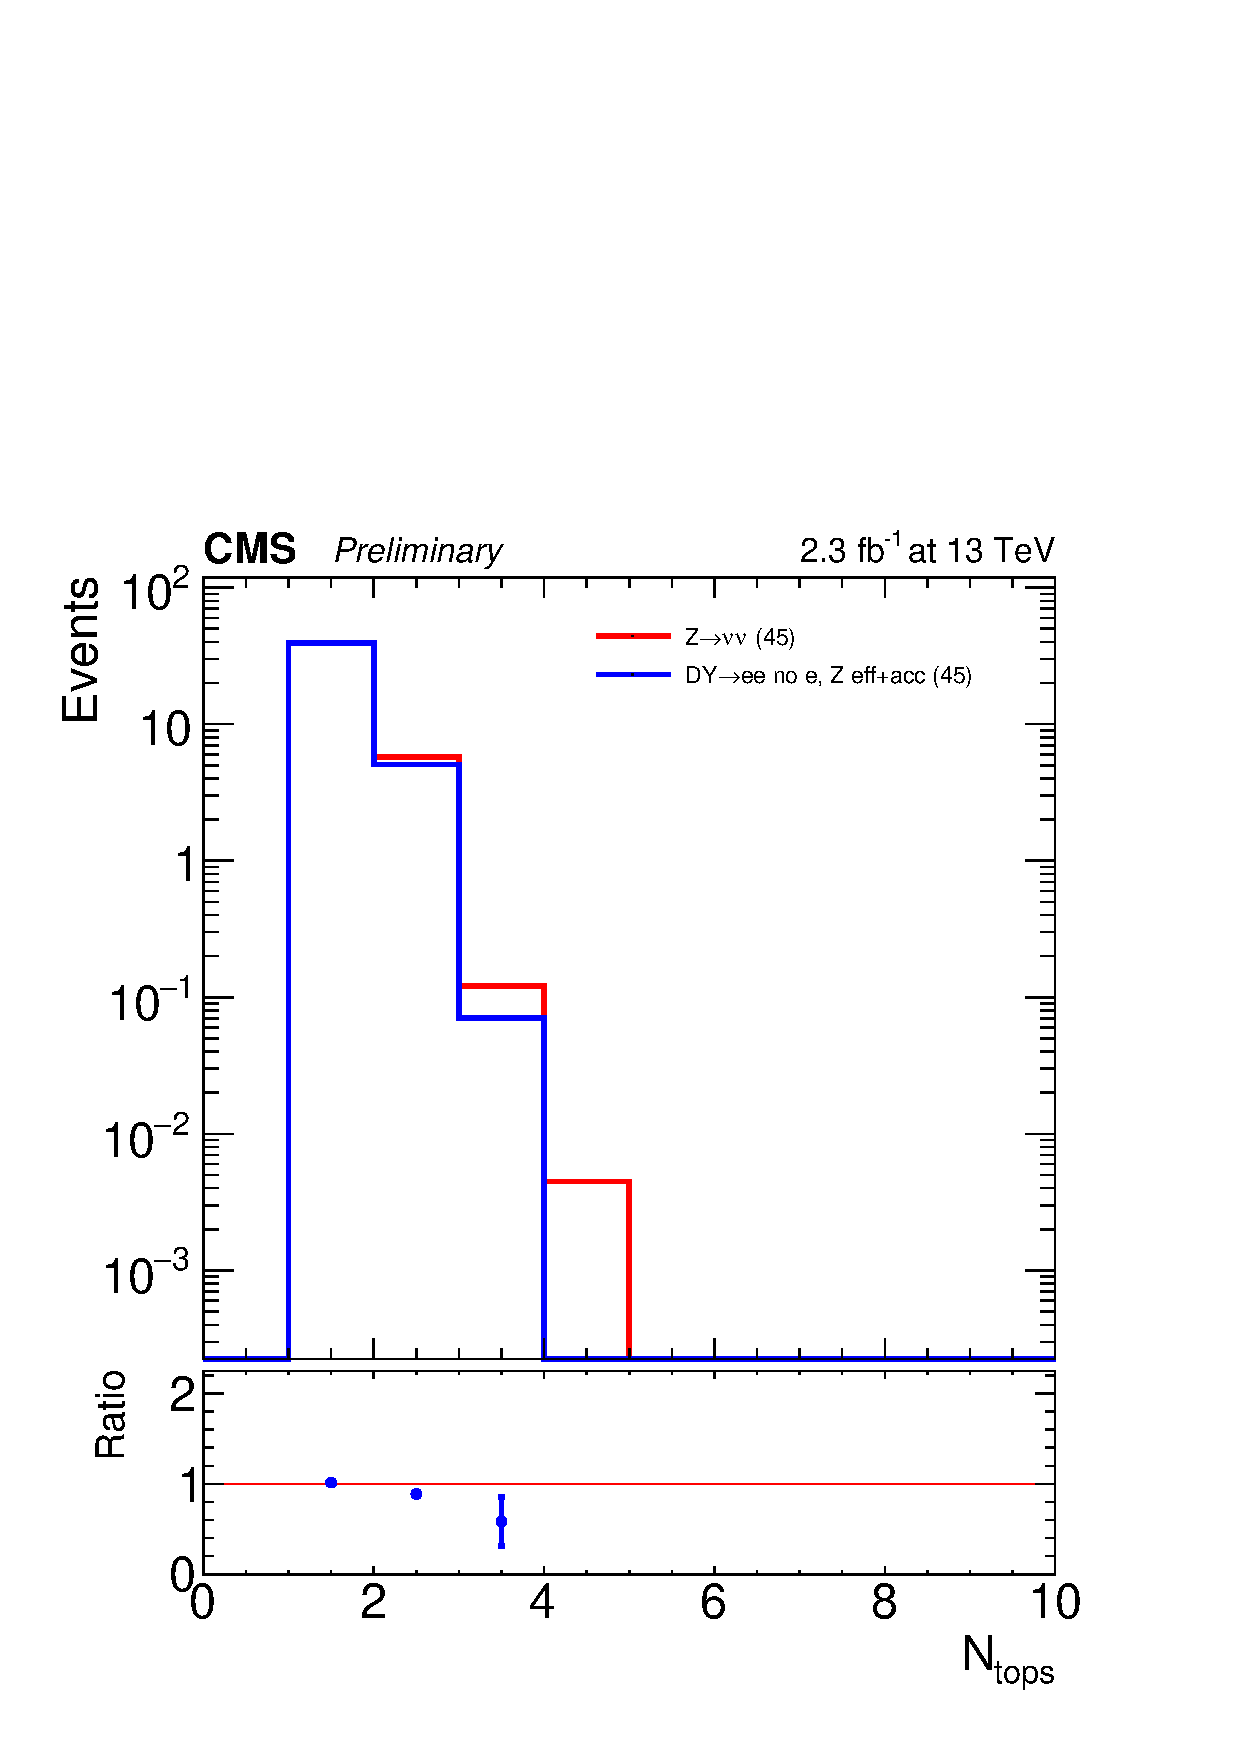
\includegraphics[width=0.5\linewidth]{figures/SusySearches/HadStop2015/MCClosure_elec_baseline_nTop.pdf}
}
\caption{Comparison of $\zinv$ prediction (blue) and expectation (red) for the b-jet multiplicity (1) and top tag multiplicity (2), after the baseline selection of the 2015 hadronic stop analysis. The ratio is of the prediction to the expectation. All events are from simulation.}
\label{fig:ZInvBaseline_NbNt}
\end{figure}
\begin{figure}[tb!]
\centering
\subfloat[]{
\includegraphics[width=0.5\linewidth]{figures/SusySearches/HadStop2015/ZinvEle_LooseHt.pdf}
}
\subfloat[]{
\includegraphics[width=0.5\linewidth]{figures/SusySearches/HadStop2015/ZinvEle_LooseMet.pdf}
}\\
\subfloat[]{
\includegraphics[width=0.5\linewidth]{figures/SusySearches/HadStop2015/ZinvEle_LooseNj.pdf}
}
\subfloat[]{
\includegraphics[width=0.5\linewidth]{figures/SusySearches/HadStop2015/ZinvEle_LooseMt2.pdf}
}
\caption{Comparison of $\zinv$ prediction (blue) and expectation (red) for the $\Ht$ (1) and $\met$ (2), the jet multiplicity (3) and the $M_{T2}$ (4), after a loosened baseline selection for the 2015 hadronic stop analysis. The ratio is of the prediction to the expectation. All events are from simulation.}
\label{fig:ZInvCR_MetHtNjMt2}
\end{figure}

\begin{figure}[tb!]
\centering
\subfloat[]{
\includegraphics[width=0.5\linewidth]{figures/SusySearches/HadStop2015/ZinvEle_LooseNb.pdf}
}
\subfloat[]{
\includegraphics[width=0.5\linewidth]{figures/SusySearches/HadStop2015/ZinvEle_LooseNt.pdf}
}
\caption{Comparison of $\zinv$ prediction (blue) and expectation (red) for the b-jet multiplicity (1) and top tag multiplicity (2), after the loosened baseline selection for the 2015 hadronic stop analysis. The ratio is of the prediction to the expectation. All events are from simulation.}
\label{fig:ZInvCR_NbNt}
\end{figure}
\noindent
The prediction and expectation agree to within a few percent across all distributions, indicating the soundness of the method; in other words, the method closes. I note that the closure holds in the region of low to moderate $\met$, where it was previously determined that large nonexcluded SUSY signals could be manifest (see Chapter \ref{chap:run1pmssm}). The method is now at a stage where it can be applied in a fully data-driven prediction. 

\FloatBarrier
\subsection{Applying the method in data}
The final $\zinv$ prediction used in \cite{CMS:2016nhb} relies on a reweighting of simulated $\zinv$ events to account for differences between data and simulation. Weights are derived in bins of $\njets$ and $\nbjets$ by dividing the counts observed in a real dilepton data sample, which has been treated with the data-driven background estimation (Equation \ref{eq:zinv}), by the counts predicted directly by $\zinv$ simulation, after a loosened baseline selection has been applied. The loose selection is defined similarly to the baseline selection, but with
\begin{itemize}
\item $\Ht>200$ GeV;
\item $\met>0$ GeV;
\item $\mttwo>0$ GeV;
\end{itemize}

The weights derived from the dielectron sample are compared with those based on the dimuon sample in Fig. \ref{fig:ZInvWeights}. 
\begin{figure}[tb!]
\centering
\subfloat[]{
\includegraphics[width=0.5\linewidth]{figures/SusySearches/HadStop2015/NJetWeightElVsMu_0b.pdf}
}
\subfloat[]{
\includegraphics[width=0.5\linewidth]{figures/SusySearches/HadStop2015/NJetWeightElVsMu_1b.pdf}
}
\caption{Comparison of data/simulation event weights for the $\zinv$ prediction based on the electron sample (green) and the muon sample (magenta) for the b-jet multiplicity 0 (left) b-jet multiplicity greater than 0 (right), after the loosened baseline selection for the 2015 hadronic stop analysis. The denominator of the weights are the counts taken from on $\zll$ simulation, and the numerator is the count in $\zll$ data where the t$\bar{\text{t}}$ contribution has been subtracted using simulation. }
\label{fig:ZInvWeights}
\end{figure}
For events with no b-tagged jets, the weights from the dielectron and dimuon sample agree within the statistical uncertainties. For events with one or more b-tagged jet, at least one bin of jet multiplicity shows a noticeable departure between the two methods. It remains to be determined if this effect is statistical in nature, or if it represents a systematic difference between the electron and muon methods. Examination of the data collected in 2016 can play an important role in answering this question.

An overall simulation-to-data normalization factor is derived in a control region with 0 b-tagged jets and applied to the $\zinv$ simulation as part of the final prediction. A comparison of the normalization factor derived from the dielectron sample with that derived from the dimuon sample is shown in Fig. \ref{fig:ZInvNorm}.
\begin{figure}[tb!]
\centering
\includegraphics[width=0.4\linewidth]{figures/SusySearches/HadStop2015/NormFactors.pdf}
\caption{The data-simulation normalization factor computed from the dimuon sample (magenta), the dielectron sample (green), and the combined dielectron $+$ dimuon sample (red). }
\label{fig:ZInvNorm}
\end{figure}
\noindent
The electron- and muon-derived normalization factors agree within statistical uncertainties, indicating that a trivial combination of the electron and muon data is justifiable in the derivation of the normalization factor and its uncertainty. After combining the electron and muon prediction samples, the systematic uncertainty in the $\zinv$ prediction associated with the normalization is reduced by approximately 30\%. Uncertainties are discussed now.

\FloatBarrier
\subsection{Uncertainties in the prediction}
Uncertainties in the $\zinv$ prediction include the statistical uncertainty of the simulated samples, uncertainty in the normalization, uncertainty associated with differences between real and simulated data, the statistical uncertainty in the $\njets-\nbjets$ weights, and other. 

The statistical uncertainty in the prediction is the bin-by-bin poisson uncertainty in the weighted simulated $\zinv$ counts. These uncertainties are negligible for the analysis \cite{CMS:2016nhb}.

The statistical uncertainty in the normalization, as well as uncertainties in the $\njets-\nbjets$ weights, are propagated to the signal region, and treated as correlated across all search regions.

Uncertainties associated with the differences in the shapes of simulated and real distributions are computed bin-by-bin in the so-called loose $N_{\text{top}}$ region, defined analogously to the baseline selection but with no criterion placed on the multiplicity of top-tagged jets. For each search bin, four comparisons are made between the data and reweighted simulated counts, one for each of the four observables, $\met$, $\mttwo$, $\nbjets$, and $N_{\text{top}}$. All but the observable considered are integrated over their full ranges, and the observable considered is integrated over the values set by the search bin for that observable. The maximum discrepancy among the four comparisons is taken as a percent uncertainty in the predicted $\zinv$ count in the bin. Comparisons of dilepton data treated with the data-driven method and reweighted simulation are shown in Fig. \ref{fig:zinvdatamc}. Uncertainties are taken to be uncorrelated across bins.


\begin{figure}[tb!]
\centering
\subfloat[]{
\includegraphics[width=0.5\linewidth]{figures/SusySearches/HadStop2015/DataMCw_SingleMuon_met_muZinv_loose0_ntop.pdf}
}
\subfloat[]{
\includegraphics[width=0.5\linewidth]{figures/SusySearches/HadStop2015/DataMCw_SingleMuon_mt2_muZinv_loose0_ntop.pdf}
}\\
\subfloat[]{
\includegraphics[width=0.5\linewidth]{figures/SusySearches/HadStop2015/DataMCw_SingleMuon_nb_muZinv_loose0_ntop.pdf}
}
\subfloat[]{
\includegraphics[width=0.5\linewidth]{figures/SusySearches/HadStop2015/DataMCw_SingleMuon_nt_muZinv_loose0_ntop.pdf}
}
\caption{Comparisons between reweighted simulation and dilepton data.}
\label{fig:zinvdatamc}
\end{figure}

The values of the uncertainties, along with the bin-by-bin prediction, for the search for SUSY in events with top-tagged jets, are given in Section \ref{sec:2015results}.

\FloatBarrier




\section{Results of 2015 SUSY searches}
\label{sec:2015results}
The QCD background estimation, $\zinv$ background estimation, and trigger techniques just described were carried out in the context of two CMS SUSY searches. This section briefly describes these analyses, their baseline selection and search region definitions, the primary backgrounds, and an interpretation of their findings in terms of various simplified models. 

This section also gives the predictions and systematic uncertainties of the background estimation methods in the search bins of the two hadronic analyses, and interpretation of the results in the context of various simplified SUSY models. Upper limits are placed on the mass of the gluino between 1400 and 1600 GeV, depending on the model, and assuming a massless LSP. Limits on the top squark mass are set around 800 GeV, assuming a massless LSP. I note that the following results are the product not only of myself, but also the work of dozens of analysis team members. I provide a high degree of detail when referring to work that was specifically carried out by me. The searches are based on a sample of proton-proton collision data collected at $\sqrt{s}=13~\TeV~$ with the CMS detector at the CERN LHC in 2015, corresponding to an integrated luminosity of 2.3 fb$^{-1}$.

\subsection{Multi-jet $+$ $\mht$ SUSY search: targeting gluino production at $\sqrt{s}=13$ TeV}
\label{sec:ra2b2015}

This search \cite{Khachatryan:2016kdk} looks for an excess of events
with four or more jets,
no identified and isolated electron, muon,
or isolated charged track,
large $\Ht$, and large $\mht$.
The principal standard model backgrounds are
 events with top quarks,
W bosons and jets,
Z bosons and jets,
and QCD multi-jet production,
and are evaluated using control samples in the data as well 
as information based on simulated events.

The search targets simplified model scenarios corresponding to  
gluino pair production.
In the various models, the gluino decays 100\% of the time into: 
 an LSP and  a light flavor q$\bar{\text{q}}$ pair (T1qqqq model), 
 an LSP and a t$\bar{\text{t}}$ pair  (T1tttt model), 
 an LSP and a b$\bar{\text{b}}$ pair (T1bbbb model).
Also considered is a model in which the gluino decays into
a q$\bar{\text{q}}$ pair and
a next-to-lightest EWkino, $\tilde{\chi}^{0}_{2}$ or $\chi^{\pm}_{1}$ (T5VV model), where 
the masses of the intermediate $\tilde{\chi}^{0}_{2}$ and $\tilde{\chi}^{\pm}_{1}$  states
are taken to be the mean of $m_{\tilde{\chi}^{0}_{1}}$ and $m_{\tilde{\text{g}}}$.
These four models are shown in 
Fig. \ref{fig:Ra2bSMS}.
\begin{figure}[tb!]
\centering
\includegraphics[width=0.45\textwidth]{figures/SusySearches/Ra2b2015/T1qqqq.pdf}
\includegraphics[width=0.45\textwidth]{figures/SusySearches/Ra2b2015/T1tttt.pdf}\\
\includegraphics[width=0.45\textwidth]{figures/SusySearches/Ra2b2015/T1bbbb.pdf}
\includegraphics[width=0.45\textwidth]{figures/SusySearches/Ra2b2015/T5vv.pdf}
\caption{
  The simplified models used for the optimization and interpretation of the multi-jet $+$ $\mht$ search. 
  They are T1qqqq (upper left), T1tttt (upper right), T1bbbb (lower left), and T5VV (lower right) scenarios.
}
\label{fig:Ra2bSMS}
\end{figure}

Events are collected using the hadronic trigger
\begin{itemize}
  \item \texttt{HLT\_PFHT350\_PFMET100\_*},
\end{itemize}
where PFHT and PFMET refer to the online $\Ht$ and $\met$ computed using the particle flow (PF) algorithm (Section \ref{sec:reconstruction}), and the numbers 350 and 100 refer to the respective triggering thresholds in units of GeV.

At level 1 of the trigger system, events are triggered if they have a calorimeter-based $\Ht$ of 175 GeV. If the event is accepted, the HLT trigger then requires a calorimeter-based $\Ht>$ 280 GeV and a calorimeter-based $\met>$ 70 GeV. Finally, the HLT trigger applies a lower threshold of 350 GeV on the $\Ht$ in coincidence with a threshold on the $\met$ above 100 GeV computed using all particles reconstructed from information from the tracker and calorimeters.

\begin{figure}[tb!]
  \begin{center}
    \includegraphics[width=0.95\linewidth]{figures/trigger/EfficiencyRatioMethodTruth.pdf}
    \caption{
      The ratio of the trigger efficiency for events passing the single
      electron reference trigger to the trigger efficiency for all
      events in a simulated t$\bar{\text{t}}$ sample, as a function of the offline $\Ht$
      and $\mht$. The ratio is consistent with 1 within the region of
      the baseline selection of $\Ht>500$ GeV and $\mht>200$ GeV of the CMS hadronic searches.
    }
    \label{fig:2dEffRatio}
  \end{center}
\end{figure}
It is seen that the choice of reference trigger, namely the single electron trigger,
\begin{itemize}
  \item \texttt{HLT\_Ele27\_eta2p1\_WPLoose\_Gsf\_v*}, 
\end{itemize}
allows for an unbiased estimate of the trigger efficiency in the region $\mht>150$ GeV and $\Ht>500$. The region in which the efficiency can be measured without bias includes the baseline selection, which imposes thresholds on the offline $\mht$ and $\Ht$ of 200 and 500 GeV. 

The efficiency, estimated without bias using Equation \ref{eq:trigeff}, is shown as a function of the offline $\Ht$ and $\mht$ in Fig. \ref{fig:trigger-turnon}, where the entire 2015 dataset has been used. 
\begin{figure}[tb!]
  \begin{center}
    \includegraphics[width=0.49\linewidth]{figures/trigger/EffVsHt2_3InvFb.png}
    \includegraphics[width=0.49\linewidth]{figures/trigger/EffVsMht2_3InvFb.png}
    \caption{
      The trigger efficiency for \texttt{HLT\_PFHT350\_PFMET100*} 
      as a function of the search variables $\Ht$ and $\mht$. The dashed (solid) blue
      lines show the distributions of the denominator (numerator) samples. These results were used in the CMS PAS on the commissioning of 13 TeV observables for SUSY searches~\cite{CMS-DP-2015-035}.
      }
    \label{fig:trigger-turnon}
  \end{center}
\end{figure}
The statistical uncertainties in the plot correspond to the 68\% CL Clopper-Pearson
interval~\cite{Clopper:Pearson}. Additionally, a systematic uncertainty is assigned to the efficiency
equal to the difference between the efficiency obtained from applying the method described to a
sample of simulated t$\bar{\text{t}}$ events and that derived
from a set of simulated signal events. Such discrepancies may arise due to any number of subtle differences in the content of the events in t$\bar{\text{t}}$ and signal samples. 

The probability for the trigger to fire on an event that passes the baseline selection is greater than 97\%. The baseline event selection can be summarized as follows. Events are accepted if they have
\begin{itemize}
\item no reconstructed, isolated lepton with a $\pt>10$ GeV and $|\eta|<2.4$, where the isolation is as defined in Equation \ref{eq:isolation};
\item no reconstructed, isolated particle track with a $\pt>10$ GeV and $|\eta|<2.4$;
\item $\Ht>500$ GeV;
\item $\mht>200$ GeV;
\item $\njets\geq$ 4, where jets are required to have a $\pt>30$ GeV and $|\eta|<2.4$, and
\item $\Delta\phi(\mht$, jet$_{1,2,3,4})>$ 0.5, 0.5, 0.3, 0.3.
\end{itemize}
After this selection, events are further subdivided into 72 exclusive bins
in a four-dimensional array of $\mht$,
the number of jets,
the number of tagged bottom quark jets,
and $\Ht$. Figure \ref{fig:ra2bArray} shows the boundaries of 6 bins in the $\Ht-\mht$ plane, and 12 bins in the plane of $\njets$$-$$\nbjets$. The 72 bins included in this search are defined by each unique combination of a box in the $\mht$$-$$\Ht$ plane and a box in the $\njets$$-$$\nbjets$ plane. The bin numbering scheme is given in Appendix \ref{app:anatables}.
\begin{figure}[tb!]
\centering
\includegraphics[height=0.442\textwidth]{figures/SusySearches/Ra2b2015/aux/MC_BG_Pie_NB0.pdf}
\hspace{-1cm}
\includegraphics[height=0.445\textwidth]{figures/SusySearches/Ra2b2015/aux/MC_BG_Pie_vs_NJets_NBJets.pdf}
\caption{The signal region boundaries in the planes of $\mht$$-$$\Ht$ (top) and $\njets$$-$$\nbjets$ (bottom) for the multi-jet $+$ $\mht$ 
search. The pie charts represent the relative contributions
 to the~\sm~backgrounds in the region $\njets=$ 4$-$6, $\nbjets=0$ (top), and $\mht=$ 200$-$500 GeV, $\Ht=$ 500$-$750 GeV (bottom).}
\label{fig:ra2bArray}
\end{figure}


\subsubsection{Background estimation}
The relative contribution of each standard model background in selected regions is also shown in Fig. \ref{fig:ra2bArray}. The t$\bar{\text{t}}$, W$+$jets, and Z$+$jets backgrounds are estimated by data-driven methods detailed in  \cite{Khachatryan:2016kdk}, but are not discussed thoroughly here. The QCD background is largest in regions of low $\mht$ and high $\Ht$, and its bin-by-bin estimation is detailed here.

The QCD background is estimated using two independent data-driven methods, one making use of a control region defined analogously to the baseline selection but with the $\Delta\phi$ requirement inverted, and by the rebalance and smear method described in Section \ref{sec:qcd}. The two methods are considered independent because the predictions are derived from nearly disjoint data control samples, and because they use different methodology. 

In the $\Delta\phi$ method, the counts in the inverted $\Delta\phi$ control region are related to the counts in the signal region by factors derived using a combination of input from real and simulated data. The information from the real data comes from events in the least sensitive search bins so as to minimize potential signal contamination. In this method, other standard model backgrounds are subtracted using estimates derived by the data-driven methods employed in the search. The largest sources of uncertainty come from the estimates of the standard model backgrounds that are subtracted. Further details about the inverted $\Delta\phi$ method are given in the literature.

The bin-by-bin prediction based on the rebalance and smear method, along with the systematic uncertainties described in Section \ref{sec:qcd}, are shown in Fig. \ref{fig:2015CompareQCD}, with the predictions and uncertainties based on the inverted $\Delta\phi$ method superimposed. The uncertainties in the rebalance and smear counts are derived based on the methodology described in Section \ref{sec:qcd}. For rebalance and smear, the largest uncertainty in bins with a large count is the uncertainty in the jet energy resolution, ranging from 10$-$30\%. In bins with exceptionally small predicted counts, the statistical uncertainty is dominant, ranging from 20$-$40\%. In bins with three or more b-tagged jets, the non-closure uncertainty is the largest, at 50\%. 
\begin{figure}[tb!]
\centering
\includegraphics[width=\linewidth]{figures/SusySearches/Ra2b2015/2015CompareQCDErrors.pdf}
\caption{ The QCD prediction based on the inverted $\Delta\phi$ extrapolation method compared with that of the of rebalance and smear method. Each type of uncertainty in the rebalance and smear prediction appears as a color-filled rectangle centered on the predicted value, summed in quadrature with the inner uncertainties. Uncertainties in the inverted $\Delta\phi$ prediction are the statistical systematic uncertainties reported in \cite{Khachatryan:2016kdk}, summed in quadrature.}
\label{fig:2015CompareQCD}
\end{figure}

No evidence of inconsistency is seen between the two predictions. The distribution of the fractional differences in the predictions of the two methods, divided by the uncertainty in the fraction (significance), is shown in Fig. \ref{fig:fractionalUnc} (a). After fitting the significance distribution  with a Gaussian function, as shown in the Figure, the best fit values for the mean and standard deviation indicate consistency between the two predictions.
\begin{figure}[tb!]
\centering
\includegraphics[width=0.49\textwidth]{figures/SusySearches/Ra2b2015/FractionalUncertainty.pdf}
\includegraphics[width=0.49\textwidth]{figures/SusySearches/Ra2b2015/FracUnc.pdf}
\caption{Left: the distribution of the significance of the deviation between the predictions from the inverted $\Delta\phi$ and rebalance and smear methods. Right: the distribution of the fractional uncertainties in the counts predicted by the two methods. The upper overflow bin is populated by bins for which the prediction is identically 0. }
\label{fig:fractionalUnc}
\end{figure}
Fig. \ref{fig:fractionalUnc} (b) shows the distribution of fractional uncertainties in the inverted $\Delta\phi$ and rebalance and smear predictions. It is seen that the inverted $\Delta\phi$ method has a prediction of zero for 22 of the search bins, whereas the rebalance and smear method gives a non-zero prediction for all but four bins. The fractional uncertainties in the rebalance and smear predictions are, overall, much smaller than those of the inverted $\Delta\phi$ predictions. This is the case in all 72 bins, except for bin 21, where the 50\% non-closure uncertainty in the rebalance and smear prediction renders an overall larger uncertainty. The bi-modal shape of the rebalance and smear distribution in Fig. \ref{fig:fractionalUnc} (b) is due to the b-tag non-closure systematic uncertainty; this uncertainty is responsible for the peak around 0.5.  Bin 35 was found to have an error in its kinematic definition, and so the prediction from the inverted $\Delta\phi$ method has been used in its stead.



\subsubsection{Results and interpretation}
The observed numbers of events in the 72 search bins
are shown in the Table in Appendix \ref{app:anatables}, along with the summed predictions for the SM backgrounds. The predicted background is observed to be compatible
with the data in all 72 regions, within uncertainties. Therefore, I do not observe evidence for new physics.
These results are interpreted in the context of the simplified models shown in Fig. \ref{fig:Ra2bSMS}.

These results are interpreted in terms of limits on the signal cross section
as a function of the gluino and LSP mass.
A likelihood function $\mathcal{L}$ is constructed as the product of Poisson probability functions,
one for each search bin, with various nuisance parameters accounting
for the yields of the four background classes and the signal strength modifier.
$\mathcal{L}$ also contains log-normal density functions that constrain the background 
yields by their estimated uncertainties. Uncertainties in the signal yield are associated
with the renormalization and factorization scales, ISR, the jet energy scale, the b-tagging efficiency,
and statistical uncertainties based on the simulated sample sizes, and are determined
as functions of $m_{\tilde{\chi}^{0}_{1}}$ and $m_{\tilde{\text{g}}}$.

The test statistic is
$q_\mu =  - 2 \ln \left( \mathcal{L}_\mu/\mathcal{L}_\text{max} \right)$,
where $\mathcal{L}_\text{max}$ is the maximum likelihood
determined by a best fit to all parameters, including the signal strength modifier,
and $\mathcal{L}_\mu$ is the maximum likelihood for a fixed signal strength.
Asymptotic formulae \cite{Cowan:2010js}
and the CL$_\mathrm{s}$ \cite{Junk1999,bib-cls} are used to set limits. 

Upper limits on the sparticle masses are identified as the set of points 
for which the 95\% confidence level upper limit on the cross section is equal to
the SUSY signal cross section computed at NLO+NLL. Expected limits are 
derived by evaluating the test statistic assuming Poisson fluctuations around
the predicted numbers of background events.

The limits are shown in Figs. \ref{fig:limitsT1qqqq}$-$\ref{fig:limitsT5vv}. For a massless LSP, gluinos are excluded with masses below 1460, 1550, 1600, and 1470 GeV,
for the T1qqqq, T1tttt, T1bbbb, and T5VV scenarios. The bands on the observed exclusion curves show the effect of varying the signal cross section by changing the renormalization and factorization scales by a factor of 2 and using the PDF4LHC recommendation~\cite{Botje:2011sn} for the PDF uncertainty. This shows the sensitivity of the limits to uncertainties in the signal cross section. 

The expected limits based on the rebalance and smear prediction are comparable to those based on the inverted $\Delta\phi$ extrapolation.  Observed limits on the gluino and LSP masses in the T1qqqq, T1tttt, and T5VV models are stronger for rebalance and smear by 20$-$50 GeV, in the compressed region. In the uncompressed region, the T1qqqq and T5VV limits are stronger by 10 and 50 GeV with the rebalance and smear prediction. In all other comparisons, the observed mass limits are nearly indistinguishable. The difference in color between left and right plots shows the comparison in the upper limit on the signal cross section between the two methods, throughout the $m_{\tilde{\text{g}}}-m_{\tilde{\chi}_{1}^{0}}$ plane. In the compressed region of the T1tttt model, the limits using input from the rebalance and smear prediction represent the strongest limits of any published CMS result, at the time of this writing. The same is true for the T5VV model, throughout the $m_{\tilde{\text{g}}}-m_{\tilde{\chi}_{1}^{0}}$ plane.

These limits significantly surpass those that were
set at $\sqrt{s}=8$ TeV,
for which the corresponding limits are around
1150 GeV \cite{Chatrchyan:2013wxa,Chatrchyan:2014lfa} for the
three T1 models and 1280 GeV \cite{Chatrchyan:2014lfa} for the T5VV model.
\begin{figure*}[tb!]
\centering
    \includegraphics[width=0.48\textwidth]{figures/SusySearches/Ra2b2015/SMSqqqqXSEC.pdf}
    \includegraphics[width=0.48\textwidth]{figures/SusySearches/Ra2b2015/SMSqqqqXSEC_rps.pdf}
    \caption{Observed (black contour) and expected (red contour) limits on the masses of the gluino and LSP using the QCD estimate based on the inverted $\Delta\phi$ method (left) and the rebalance and smear method (right), in the context of the T1qqqq model. The dashed (grey) lines indicate the $\tilde{\chi}^{0}_{1}=m_{\tilde{\text{g}}}$ diagonal.}
    \label{fig:limitsT1qqqq}
\end{figure*}
\begin{figure*}[tb!]
\centering
    \includegraphics[width=0.48\textwidth]{figures/SusySearches/Ra2b2015/SMSttttXSEC.pdf}
    \includegraphics[width=0.48\textwidth]{figures/SusySearches/Ra2b2015/SMSttttXSEC_rps.pdf} \\
    \caption{Observed (black contour) and expected (red contour) limits on the masses of the gluino and LSP using the QCD estimate based on the inverted $\Delta\phi$ method (left) and the rebalance and smear method (right), in the context of the T1tttt model.}
    \label{fig:limitsT1tttt}
\end{figure*}
\begin{figure*}[tb!]
\centering
    \includegraphics[width=0.48\textwidth]{figures/SusySearches/Ra2b2015/SMSbbbbXSEC.pdf}
    \includegraphics[width=0.48\textwidth]{figures/SusySearches/Ra2b2015/SMSbbbbXSEC_rps.pdf} \\
    \caption{Observed (black contour) and expected (red contour) limits on the masses of the gluino and LSP using the QCD estimate based on the inverted $\Delta\phi$ method (left) and the rebalance and smear method (right), in the context of the T1bbbb model.}
    \label{fig:limitsT1bbbb}
\end{figure*}
\begin{figure*}[tb!]
\centering
    \includegraphics[width=0.48\textwidth]{figures/SusySearches/Ra2b2015/SMSqqqqVVXSEC.pdf}
    \includegraphics[width=0.48\textwidth]{figures/SusySearches/Ra2b2015/SMSqqqqVVXSEC_rps.pdf}
    \caption{The observed (black contour) and expected (red contour) limits on the masses of the gluino and LSP using the QCD estimate based on the inverted $\Delta\phi$ method (left) and the rebalance and smear method (right), in the context of the T5VV model. }
    \label{fig:limitsT5vv}
\end{figure*}


\FloatBarrier

\subsection{Search for SUSY in events with top-tagged jets at $\sqrt{s}=13$ TeV}
\label{sec:hadstop2015}
This search \cite{CMS:2016nhb} looks for evidence of SUSY in events with jets identified as top quarks. An excess of events containing top-tagged jets (top tags) over the standard model background may be evidence of the production of top squark pairs, whose existence has been motivated as a solution to the hierarchy problem (Section \ref{sec:problems}).  The possibility of top squarks with masses below about 450 GeV has largely been ruled out by results from other experiments (Chapter \ref{chap:run1pmssm}).  However, considerations of naturalness implore us to look for evidence of top squarks nonetheless. The analysis is optimized to be sensitive to signatures resembling the simplified models shown in Fig. \ref{fig:hadstopSMS}.
\begin{figure}[h]
\centering
\includegraphics[width=0.45\textwidth]{figures/SusySearches/HadStop2015/T2tt.pdf}
\includegraphics[width=0.45\textwidth]{figures/SusySearches/HadStop2015/T1tttt.pdf}\\
\caption{
  The simplified models used for the optimization and interpretation of the hadronic search for SUSY in events with top-tagged jets. They are T2tt (left) and T1tttt (right).
}
\label{fig:hadstopSMS}
\end{figure}

In addition to the multiplicity of top tags, other observables are used for signal/background discrimination, including the $\Ht$, $\met$, $\njets$, $\nbjets$, and the stransverse mass $M_{\text{T2}}$~\cite{Lester:1999tx}. Top tags are constructed by considering all three-jet combinations in an event, and selecting a combination with an invariant mass consistent with the top quark mass. Additional topological requirements are placed on the top-tagged jet to reject background from QCD jet combinations. After identifying a top-tagged jet, the remaining jets in the event are analyzed and checked for consistency with a second top quark in the event, inferred by the presence of a b-tagged jet. In the event that both systems (the top-tagged system and the remnant b-tagged jet) are reconstructed, the $M_{\text{T2}}$ is computed taking the four-vectors of the two top candidates as input, along with the $\met$ of the event. 

Events are collected using the same hadronic trigger used in the work of the previous section,
\begin{itemize}
  \item \texttt{HLT\_PFHT350\_PFMET100\_*}.
\end{itemize}
The probability for the trigger to accept an event that passes the baseline selection is greater than 98\%. For the baseline selection, events are selected if they have
\begin{itemize}
\item no reconstructed, isolated muon with a $\pt>10$ GeV, $|\eta|<2.4$, and isolation $<0.2$;
\item no reconstructed, isolated electron with a $\pt>10$ GeV, $|\eta|<2.5$, and isolation $<0.1$;
\item no reconstructed, isolated lepton (hadron) track with a $\pt>5$ (10) GeV, $|\eta|<2.5$, and isolation $0.2$;
\item $\Ht>500$ GeV;
\item $\met>200$ GeV;
\item $\Delta\phi(\mht$, jet$_{1,2,3})>$ 0.5, 0.5, 0.3;
\item $N_t\geq1$, where $N_t$ is multiplicity of top tags;
\item $\nbjets\geq1$, and
\item $M_{\text{T2}}>200$ GeV.
\end{itemize}
After the baseline selection, events are further subdivided into 37 search bins defined by rectangular boundaries in the dimensions of $\met$, $M_{\text{T2}}$, $\nbjets$, and $N_t$, with boundaries and bin numbers shown in Fig. \ref{fig:hadstopArray}.
\begin{figure}[h]
  \begin{center}
    \includegraphics[width=0.45\linewidth]{HadStopPaper/figures/poly_MT2_vs_met_merged_0.pdf}
    \includegraphics[width=0.45\linewidth]{HadStopPaper/figures/poly_MT2_vs_met_merged_1.pdf} \\
    \includegraphics[width=0.45\linewidth]{HadStopPaper/figures/poly_MT2_vs_met_merged_3.pdf} 
    \includegraphics[width=0.45\linewidth]{HadStopPaper/figures/poly_MT2_vs_met_merged_4.pdf} \\
    \caption{ Search bin definitions after baseline selection cuts. }
    \label{fig:hadstopArray}
  \end{center}
\end{figure}

The most significant background comes from the SM t$\bar{\text{t}}$ production or W-boson production in association with jets, where the ${\rm W}$ decays into leptons that are either not accepted, not reconstructed, or not isolated. The next largest contribution comes from $\zinv$ production in association with jets, including b-jets, in which the neutrino pair gives rise to large $\met$ and the top quark conditions are satisfied by an accidental combination of the jets. The QCD multi-jet contribution and the contribution from other rare SM processes are subdominant across all search bins. 


\subsubsection{Background estimation}
The t$\bar{\text{t}}$, W$+$jets, and QCD backgrounds are estimated by data-driven methods detailed in \cite{CMS:2016nhb}, but are not discussed thoroughly here. The $\zinv$ background is most dominant in regions of small $\Ht$ and large $\met$, and its bin-by-bin estimation is detailed here.

The $\zinv$ background is estimated using the ee and $\mu\mu$ samples as a proxy for the true sample in which the Z decays into neutrinos. The method used to derive the prediction, as well as uncertainties, is that described in Section \ref{sec:zinv}. The values and uncertainties in the bin-by-bin prediction are shown in Fig. \ref{fig:2015ZinvPrediction} for the $\mu\mu$-derived prediction, the ee-derived prediction, and the prediction based on the combined $\mu\mu+$ee sample. 
\begin{figure}[tb!]
\centering
\includegraphics[width=0.6\linewidth]{figures/SusySearches/HadStop2015/moneyplotJoeMu.pdf}\\
\includegraphics[width=0.6\linewidth]{figures/SusySearches/HadStop2015/moneyplotEl.pdf}\\
\includegraphics[width=0.6\linewidth]{figures/SusySearches/HadStop2015/moneyplotLep.pdf}
\caption{ The predicted counts originating from standard model $\zinv$ production, based on the $\mu\mu$ sample (top), the ee sample (center), and the combined $\mu\mu+$ee sample (bottom). Each type of uncertainty, described in Section \ref{sec:zinv}, appears as a color-filled rectangle centered on the predicted value, summed in quadrature with the inner uncertainties. }
\label{fig:2015ZinvPrediction}
\end{figure}
The $\mu\mu$-derived and ee-derived predictions are compatible within the uncertainties, but the ee-derived prediction is systematically larger than that of the $\mu\mu$-derived prediction by at least 40\%. This is due to the difference in the normalization factor-derived in the two methods, as well as differences in the data-simulation weights. 

\subsubsection{Results and interpretation}
The predicted number of SM background events and the number of events observed in data for each of the search bins are shown in Figure~\ref{fig:baseline_SR} and Tabulated in Appendix \ref{app:anatables}. 
\begin{figure}[htbp]
  \begin{center}
  \begin{tabular}{cc}
\hspace{-1.5cm}
  \includegraphics[width=0.85\textwidth]{figures/SusySearches/HadStop2015/UnblindPlots.pdf}
  \end{tabular}
  \caption{Data are shown as black points. The total predictions are shown in filled solid area. The bottom plot shows the ratio of data over total background prediction in each search bin. Only statistical uncertainties are propagated to the ratio. The numbering scheme is given in Ref. \cite{CMS:2016nhb}.}
    \label{fig:baseline_SR}
  \end{center}
\end{figure}
The predicted background counts are observed to be compatible with the data in all 37 regions, within uncertainties. Therefore, no evidence of new physics is observed.
These results are interpreted in the context of the simplified models shown in Fig. \ref{fig:Ra2bSMS}.

%The following uncertainties on the signal modeling are taken into account when the limits are determined: simulation sample size, luminosity determination ($4.6\%$), lepton and isolated track veto, b-tag efficiency corrections used to scale simulation to data, trigger efficiency, QCD renormalisation and factorization scales, initial/final state radiation (ISR/FSR), signal acceptance and efficiency arising from the jet energy-momentum corrections, jet energy-momentum resolutions, and propagated to \MET, parton distribution functions (PDF) of the proton

The results are interpreted in terms of the simplified model scenarios shown in Fig. \ref{fig:hadstopSMS} using an analogous limit setting procedure discussed in Section \ref{sec:ra2b2015}. Uncertainties in the signal yields are similar to those discussed in Section \ref{sec:ra2b2015}, with additional uncertainties associated with differences in the top-quark tagging efficiency and false positive rate between the CMS fast and full simulations, on the order of a few percent.

%%%%%%%%%%%%%%%%%%%%%%%%%%%%%%%%%%%%%%%%%%%%%%%%%%

%-------------
Upper limits on the observed cross section for the signal models T2tt and T1tttt are shown in Figs. \ref{fig:fulllimit_T2tt} and \ref{fig:fulllimit_T1tttt}, along with contours corresponding to the expected (red) and expected (black) upper limits on the SUSY masses, assuming the assuming the NLO+NLL theoretical SUSY cross sections. In the case of T2tt, limits are shown assuming the predicted $\zinv$ counts based on the $\mu\mu$, ee, and $\mu\mu+$ee samples. For T1tttt, just the limits on the $\mu\mu$ and $\mu\mu+$ee samples are shown. 

%%%%%%%%%%%%%%%%%%%%%%%%%%%%%%%%%%%%%%%%%%%%%%%%%%
\begin{figure}[htbp]
  \begin{center}
  \begin{tabular}{cc}
\hspace{-1.5cm}
  \includegraphics[angle=0,width=0.48\textwidth]{figures/SusySearches/HadStop2015/HadStopT2tt_Mu.pdf}
  \includegraphics[angle=0,width=0.48\textwidth]{figures/SusySearches/HadStop2015/HadStopT2tt_El.pdf}\\
    \includegraphics[angle=0,width=0.48\textwidth]{figures/SusySearches/HadStop2015/HadStopT2tt_MuEl.pdf}
  \end{tabular}
  \caption{Observed (black contour) and expected (red contour) limits on the top squark and LSP masses in the context of the T2tt model. The top-left plot corresponds to the $\mu\mu$-derived $\zinv$ prediction, the top-right to the ee-derived prediction, and the bottom plot to the prediction of the combined $\mu\mu+$ee sample.}
    \label{fig:fulllimit_T2tt}
  \end{center}
\end{figure}

\begin{figure}[htbp]
  \begin{center}
  \begin{tabular}{cc}
\hspace{-1.5cm}
  \includegraphics[angle=0,width=0.48\textwidth]{figures/SusySearches/HadStop2015/HadStopT1tttt_Mu.pdf}
  \includegraphics[angle=0,width=0.48\textwidth]{figures/SusySearches/HadStop2015/HadStopT1tttt_MuEl.pdf}
  \end{tabular}
  \caption{Observed (black contour) and expected (red contour) limits on the gluino and LSP masses in the context of the T1tttt model. The left plot corresponds to the $\mu\mu$-derived prediction for the $\zinv$ counts, and the right plot to the muon$+$ee-derived prediction.}
    \label{fig:fulllimit_T1tttt}
  \end{center}
\end{figure}
%%%%%%%%%%%%%%%%%%%%%%%%%%%%%%%%%%%%%%%%%%%%%%%%%%
In the case of T2tt, the ee-derived expected limit is somewhat less constraining than that of the expected muon-derived limit, as was expected from the outset. The ee-derived observed limit on the top squark mass is actually stronger than the $\mu\mu$-derived observed limit by about 20 GeV, for small values of the LSP mass. This difference is due to the considerably larger ee-derived $\zinv$ prediction. The combined $\mu\mu$+ee-derived expected limit is comparable to the $\mu\mu$-derived expected limit. The observed limit based on the combined result is slightly more constraining on the top squark mass than the $\mu\mu$ result, by about 10 GeV, for small LSP masses. The largest observed upper limit on $m_{\tilde{\text{t}}}$ for low LSP mass comes from the ee estimate, and is approximately 780 GeV, coinciding with the expected limit. In the compressed region, the strongest observed limit comes from the ee prediction, where LSPs are excluded with masses below about 180 GeV, which is nearly in agreement with the expected limit.

In the T1tttt model, only negligible differences appear between the $\mu\mu$ and the combined $\mu\mu+$ee predictions. Given the limited constraining power of the ee control sample, this sample be better used in more creative ways, for example, as a training sample for a multivariate discriminant. This is explored in the next chapter.



\FloatBarrier

